%%------------------------------------
%% Digital Design Lab Manual 
%%  Christopher Coulston
%%------------------------------------

%%\documentclass[11pt,psfig]{book}
\documentclass[letterpaper, 10pt]{memoir}
\chapterstyle{ger}
\settrims{0pt}{0pt}
\semiisopage[9]		% [N] is spine margin is 1/Nth pf page 

\makeindex

% To keep the book.tex file clean, I pulled all the formating and package 
% includes into the preamble.tex file

%%------------------------------------------------------
%%------------------------------------------------------

\usepackage{amsmath,amssymb}
\usepackage{lmodern}
\usepackage{iftex}

\usepackage{xcolor}
\usepackage{graphicx}

\usepackage{dirtree}		% For the body of knowledge


\usepackage{listings}

\makeatletter
\def\maxwidth{\ifdim\Gin@nat@width>\linewidth\linewidth\else\Gin@nat@width\fi}
\def\maxheight{\ifdim\Gin@nat@height>\textheight\textheight\else\Gin@nat@height\fi}
\makeatother
% Scale images if necessary, so that they will not overflow the page
% margins by default, and it is still possible to overwrite the defaults
% using explicit options in \includegraphics[width, height, ...]{}
\setkeys{Gin}{width=\maxwidth,height=\maxheight,keepaspectratio}
% Set default figure placement to htbp
\makeatletter
\def\fps@figure{htbp}
\makeatother

\usepackage{longtable,booktabs,array}
\usepackage{multirow}
\usepackage{calc}
\usepackage[normalem]{ulem}

\usepackage{pdflscape}

\usepackage{bookmark}

\usepackage{xurl}

\usepackage{hyperref}

%\let\oldhypertarget\hypertarget
%\renewcommand*{\hypertarget}{\oldhypertarget\space}



\hypersetup{
   colorlinks=true,
   linkcolor=red}
\newclipboard{digitalBodyOfKnowledge}

\begin{document}

\renewcommand{\chaptername}{Laboratory}

\title{}
 
\tableofcontents
\vspace{0.4cm}
When clicking on a link in Adobe use alt+arrow left to return to where you started.

\chapter*{Objectives}
These are the objectives of the lecture
and homework sequence of the course.  They have been arranged
to parallel the chapter/section sequence in the textbook.

\dirtree{%
	.1 \Copy{bok:Digital_Design}{Digital Design}.	
	.2 \Copy{bok:Numbering_systems}{Numbering Systems}.
	.3 \Copy{bok:NS_Positional}{Positional Numbering Systems}.
	.4 \Copy{bok:NS_POS_base10}{Base 10 - Decimal}.
	.4 \Copy{bok:NS_POS_base2}{Base 2 - Binary}.
	.4 \Copy{bok:NS_POS_base16}{Base 16 - Hexadecimal}.
	.3 \Copy{bok:NS_baseConversion}{Between Bases}.
	.3 \Copy{bok:NS_Word Size}{Word Size}.
	.3 \Copy{bok:NS_Twos}{2's Complement}.
	.2 \Copy{bok:Respresentions}{Representation of Logical Function}.
	.3 \Copy{bok:REP_Elfs}{Elementary Logical Functions}.
	.3 \Copy{bok:REP_WordStatement}{Analyzing a word statement for a logic function}.
	.3 \Copy{bok:REP_TruthTable}{Creating a truth table description for a logic function}.
	.3 \Copy{bok:REP_Symbolic}{Creating a symbolic form for a logic function}.
	.3 \Copy{bok:REP_CircuitDiagram}{Creating a circuit diagram for a logic function}.
	.3 \Copy{bok:REP_HDL}{Creating Hardware Description Language statements for a logic function}.
	.3 \Copy{bok:REP_Convert}{Conversion between two different representations of a logic function}.
	.3 \Copy{bok:REP_MultiOut}{Describing a functions with multiple outputs}.	
	.3 \Copy{bok:REP_Timing}{Timing Diagrams}.
	.2 \Copy{bok:LogicMin}{Logic Minimization}.
	.3 \Copy{bok:LM_Kmap}{Karnaugh Maps (Kmaps)}.
	.3 \Copy{bok:LM_MultiOut}{Kmaps for circuits with multiple outputs}.
	.3 \Copy{bok:LM_KmapPos}{Kmaps to find POSmin}.
	.3 \Copy{bok:LM_Soft}{Using logic minimization software to describe a logic function}.
	.2 \Copy{bok:Com_Building_Blocks}{Combination Logic Building Blocks}.
	.3 \Copy{bok:CC_Dec}{Decoder}.
	.3 \Copy{bok:CC_Mux}{Multiplexers}.
	.3 \Copy{bok:CC_Adder}{Adders}.
	.3 \Copy{bok:CC_Compare}{Comparators}.
	.3 \Copy{bok:CC_WireLogic}{Wire Logic}.
	.3 \Copy{bok:CC_Glue_Combo}{Designing glue logic to interface building blocks}.
	.3 \Copy{bok:CC_Combos}{Analyzing a circuit with a combination of building blocks}.
	.4 \Copy{bok:CC_ArthStatements}{Arithmetic Statements}.
	.4 \Copy{bok:CC_ConditionalStatements}{Conditional Statements}.	
	.2 \Copy{bok:BasicMemoryElements}{Basic Memory Element Behavior}.
	.3 \Copy{bok:BME_Char}{Characteristics}.
	.3 \Copy{bok:BME_Timing}{Timing of basic memory element}.
	.3 \Copy{bok:BME_Asynch}{Asynchronous set reset}.	
	.2 \Copy{bok:BMS_Memory}{Sequential Logic Building Blocks}.	
	.3 \Copy{bok:BMS_Reg}{Analysis, design and use of a register in a digital design}.
	.3 \Copy{bok:BMS_ShitReg}{Shift Register}.
	.3 \Copy{bok:BMS_Counter}{Counter}.
	.3 \Copy{bok:BMS_Ram}{Static RAM}.
	.3 \Copy{bok:BMS_RegTran}{Design a circuit that performs register transfer}.	
	.2 \Copy{bok:FSM}{Finite State Machines}.
	.3 \Copy{bok:FSM_Hardware}{Hardware organization of a finite state machine}.
	.3 \Copy{bok:FSM_StateDiagram}{State diagram for a finite state machine}.
	.3 \Copy{bok:FSM_OneHot}{One's Hot Encoding}.
	.3 \Copy{bok:FSM_design}{Design}.
	.3 \Copy{bok:FSM_Timing}{Using a timing diagram to specify or verify the proper operation of a Finite State Machine}.
	.2 \Copy{bok:DaC}{Datapath and Control}.
	.3 \Copy{bok:DaC_Architecture}{Datapath and Control Architecture}.
	.3 \Copy{bok:DaC_Algorithm}{Algorithmic Language}.
	.3 \Copy{bok:DaC_ControWord}{Design a control word table and spcify the control word values for every state.}.
	.3 \Copy{bok:DaC_Design}{Design}.
	.3 \Copy{bok:DaC_Timing}{Using a timing for a datapath and control circuit to specify or verify proper operation.}.	
}
\vspace{0.5cm}

These are the objectives of the lab sequence in this class broken down into Verilog  and FPGA.  Verilog
objectives are agnostic to the hardware platform. FPGA objectives are specific to the
hardware and software platformed used to implement the designs laid out in 
these labs.  This organization should enable instructors to quickly identify units 
which may need to be adapted
to run the lab sequence on different hardware/software platform.
\dirtree{%
	.1 \Copy{VER}{Verilog }.
	.2 \Copy{VER:CSA}{Writing concurrent signal assignment statements for a logic function}.
	.2 \Copy{VER:Logic}{Writing a Verilog statement using primitive logic operations}.
	.2 \Copy{VER:AlwaysCase}{Writing a Verilog statement using an Always/Case statement}.	
	.2 \Copy{VER:AlwaysCaseZ}{Writing a Verilog statement using an Always/CaseZ statement}.	
	.2 \Copy{VER:Vectors}{Creating a Verilog statement that uses vectors}.
	.2 \Copy{VER:Test}{Analyzing and designing a Verilog testbench}.
	.2 \Copy{VER:Generics}{Definition and instantiation of Verilog generic modules}.	
	.2 \Copy{VER:Module}{Definition of Verilog modules}.
	.2 \Copy{VER:Instantiating}{Instantiation of Verilog Modules}.
	.2 \Copy{VER:fsm}{Definition of Finite State Machines in Verilog}.	
	.1 \Copy{HDL}{Hardware and Software Specifics}.
	.2 \Copy{HDL:Time}{Creating a simulation timing diagram for a module}.
	.2 \Copy{HDL:Pin}{Creating a pin assignment for a module}.
	.2 \Copy{HDL:Do}{Creating a Do file to automate waveform setup}.
	.2 \Copy{HDL:Synthesis}{Synthesizing a module on the FPGA development board}.
}	
		

\chapter{Introduction to Verilog}
\label{introductionToVerilog}
\graphicspath{ {./Lab01SimpleVerilog/Fig} }


\hypertarget{objective}{%
\section{\texorpdfstring{Objective }{Objective }}\label{objective}}

The objective of this lab is to introduce you to the Quartus II
software, design entry using Verilog and circuit simulation.


\hypertarget{part-1-setting-up-a-project-in-quartus-and-running-a-testbench}{%
\section{Part 1: Setting up a project in Quartus and running a testbench}
\label{part-1-setting-up-a-project-in-quartus-and-running-a-testbench}}

\begin{enumerate}
\def\labelenumi{\arabic{enumi}.}
\item
  Select an appropriate working directory for your project. I would
  recommend selecting your network drive.

  \begin{enumerate}
  \def\labelenumii{\alph{enumii}.}
  \item
    Create a new folder \emph{lab1},
  \item
    Create another folder within \emph{lab1} called \emph{andgate2},
  \item
    Download \emph{andgate2.v} and \emph{andgate2\_tb.v} from Canvas,
  \item
    Save these files in andgate2 directory.
  \end{enumerate}
\item
  Start Quartus II 18.1 (64-bit).

  \begin{enumerate}
  \def\labelenumii{\alph{enumii}.}
  \item
    If you are prompted by a License Setup choose the free option. You
    may need to restart Quartus if this happens.
  \end{enumerate}
\item
  Select \emph{File -\textgreater{} New Project Wizard.}
\item
  In the \textbf{Directory, Name, Top-Level Entity} page of the New
  Project Wizard pop-up:

  \begin{enumerate}
  \def\labelenumii{\alph{enumii}.}
  \item
    To the right of the ``What is the working directory'' box click the
    \ldots{} button,
  \item
    In the Select Folder pop-up, navigate so you can see the andgate2
    directory created in step 1,
  \item
    Select the andgate2 folder, click Select Folder,
  \item
    In the ``What is the name of this project'' field type
    \emph{andgate2}
  \item
    click \emph{Next}.
  \end{enumerate}
\item
  In the \textbf{Project Type} page of the New Project Wizard pop-up:

  \begin{enumerate}
  \def\labelenumii{\alph{enumii}.}
  \item
    Select the \emph{Empty project} radio button,
  \item
    click \emph{Next}.
  \end{enumerate}
\item
  In the \textbf{Add Files} page of the New Project Wizard pop-up:

  \begin{enumerate}
  \def\labelenumii{\alph{enumii}.}
  \item
    Click the \ldots{} button to the right of File name,
  \item
    In the Select File pop-up, navigate to, and select,
    \emph{andgate2.v} and \emph{andgate2\_tb.v}, click Open,
  \item
    The file should appear in the window below,
  \item
    Click \emph{Next}
  \end{enumerate}
\item
  In the \textbf{Family \& Device Settings} page of the New Project
  Wizard pop-up:

  \begin{enumerate}
  \def\labelenumii{\alph{enumii}.}
  \item
    Device family, Family: Cyclone V
  \item
    Package: FBGA
  \item
    Pin Count: 672
  \item
    Speed Grade: 7\_H6
  \item
    Select Specific device selected in `Available devices' list
  \item
    From the list of available devices, select: 5CGXFC5C6F27C7
  \item
    Click Next
  \end{enumerate}
\item
  In the \textbf{EDA Tool Settings} page of the New Project Wizard
  pop-up:

  \begin{enumerate}
  \def\labelenumii{\alph{enumii}.}
  \item
    In the Simulation row

    \begin{enumerate}
    \def\labelenumiii{\roman{enumiii}.}
    \item
      Tool Name column: ModelSim-Altera
    \item
      Formats column: Verilog HDL
    \end{enumerate}
  \item
    Leave other defaults alone
  \item
    Click Next
  \end{enumerate}
\item
  In the \textbf{Summary} page of the New Project Wizard pop-up:

  \begin{enumerate}
  \def\labelenumii{\alph{enumii}.}
  \item
    Review information,
  \item
    Click Finish.
  \end{enumerate}
\item
  Back in the main Quartus II window, Click \emph{Tools -\textgreater{}
  Options..}.
\item
  In the Options pop-up:

  \begin{enumerate}
  \def\labelenumii{\alph{enumii}.}
  \item
    Select \emph{EDA Tool Options} from the Category menu,
  \item
    If the last row, ``ModelSim-Altera'' is blank, click on the \ldots{}
    button at right and navigate to the
    \emph{C:\textbackslash intelFPGA\_lite\textbackslash18.1\textbackslash modelsim\_ase\textbackslash{}},
    select the \emph{win32aloem} folder, the click Select Folder,
  \item
    Click Ok.
  \end{enumerate}
\item
  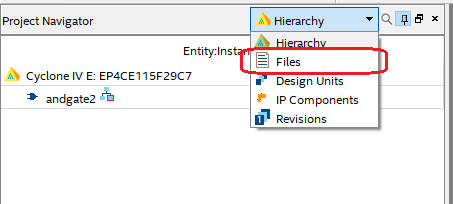
\includegraphics[width=3.9in,height=1.8in]{image1.png}Click
  on the Files tab in the \emph{Project Navigator} pane.
\item
  Right click on \emph{andgate2\_tb} in the \emph{Project Navigator}
  pane and select Set as Top-Level entity.
\item
  Double click on \emph{andgate2}.
\item
  If you added the Verilog file in the correct directory and included it
  in the project, a Verilog file should pop up on the right.
\item
  In the main Quartus II window, click on \emph{Processing
  -\textgreater{} Start -\textgreater{} Start Analysis \& Elaboration.}
  This may take some time, so be patient.
\item
  If you did everything correctly you should

  \begin{enumerate}
  \def\labelenumii{\alph{enumii}.}
  \item
    Notice that andgate\_tb is the new top-level entity in the Hierarchy
    pane. Expand the andgate2\_tb by clicking on the ``\textgreater''
    arrow to see the entities inside it.
  \item
    You should see the following messages in the console area, the
    bottom pane.
  \end{enumerate}
\end{enumerate}

\begin{quote}
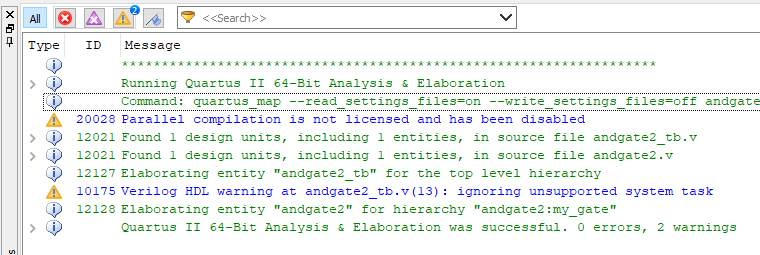
\includegraphics{image2.png}
\end{quote}

\begin{enumerate}
\def\labelenumi{\arabic{enumi}.}
\setcounter{enumi}{17}
\item
  In the main Quartus II window, click \emph{Tools -\textgreater{} Run
  Simulation Tool -\textgreater{} RTL Simulation}. The ModelSim program
  will launch. This may take a few moments, be patient. If you get a
  pop-up Nativelink Error window, then go back and check and fix the
  directory in step 11.
\item
  In ModelSim, click Simulate -\textgreater{} Start Simulation
\item
  In the Start Simulation pop-up, expand the \emph{work} library by
  clicking on the ``+'' at left. click on \emph{andgate2\_tb} and click
  \emph{Ok}.
\item
  In the sim pane, right mouse click on uut and select \emph{Add Wave}.
\end{enumerate}

\begin{quote}
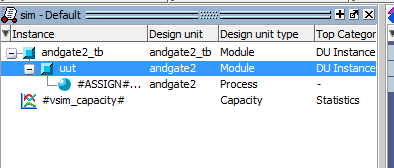
\includegraphics[width=4.10417in,height=1.75in]{image3.png}
\end{quote}

\begin{enumerate}
\def\labelenumi{\arabic{enumi}.}
\setcounter{enumi}{21}
\item
  Choose \emph{Simulate -\textgreater{} Run -\textgreater{} Run 100}.
  You should see inputs and output from andgate2. If you see only a
  small green portion of the waveform on the left margin of the timing
  diagram, you will need to zoom in on the waveform as follows. First
  click somewhere in the timing diagram (area under ``Undocking tool''
  in the image below) and then click on the ``Zoom all tool'' shown in
  following image.
\item
  \protect\hypertarget{Part_1_Step_23}{}{}Save this waveform as an image
  as follows:

  \begin{enumerate}
  \def\labelenumii{\alph{enumii}.}
  \item
    Undock the Wave pane by clicking the undocking tool icon.
  \end{enumerate}
\end{enumerate}

\begin{quote}
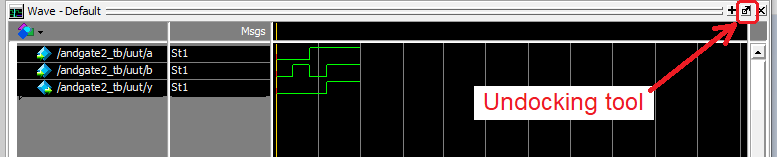
\includegraphics{image4.png}
\end{quote}

\begin{enumerate}
\def\labelenumi{\alph{enumi}.}
\setcounter{enumi}{1}
\item
  Resize the undocked Wave window vertically by grabbing its top edge
  and dragging down. Make the window tall enough to fit all the waves
  with a little room to spare.
\end{enumerate}

\begin{quote}
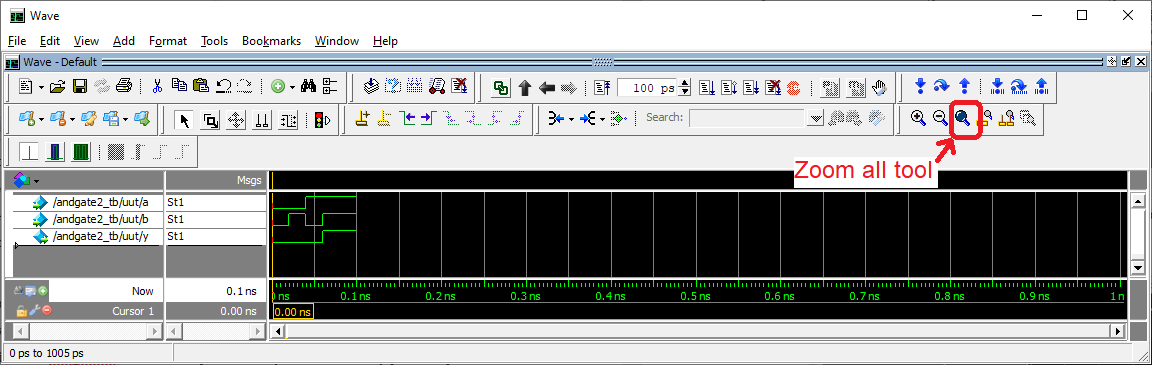
\includegraphics{image5.png}
\end{quote}

\begin{enumerate}
\def\labelenumi{\alph{enumi}.}
\setcounter{enumi}{2}
\item
  Click the Zoom all tool to file the available horizontal space with
  the waveform.
\item
  Click File -\textgreater{} Export -\textgreater{} Image
\end{enumerate}

\begin{quote}
If this does not work, you can take a screen shot of the window by
pressing Alt-Print Screen. The ``Alt'' captures the currently active
window into the graphics buffer.
\end{quote}

\begin{enumerate}
\def\labelenumi{\alph{enumi}.}
\setcounter{enumi}{4}
\item
  Navigate to your project directory, provide a File name, then click
  Save
\item
  Exit Modelsim using File -\textgreater{} Quit. Do not save wave
  commands.
\end{enumerate}

\begin{enumerate}
\def\labelenumi{\arabic{enumi}.}
\setcounter{enumi}{23}
\item
  Back in Quartus, close your current project using File -\textgreater{}
  Close Project. Save if needed.
\end{enumerate}

\hypertarget{part-2-symbolic-to-verilog-timing-diagram-truth-table.}{%
\section{Part 2: Symbolic to Verilog , Timing Diagram, Truth Table}
\label{part-2-symbolic-to-verilog-timing-diagram-truth-table.}}

Write Verilog code to realize the function \emph{f02 = a' + bc'} Note
that this symbolic expression is written using the notation used in
class. This is not a valid Verilog expression.

\begin{enumerate}
\def\labelenumi{\arabic{enumi}.}
\item
  Create \textbf{a new project} folder within your \emph{lab1} directory
  called \emph{function02.}
\item
  Download \emph{function02.v} and \emph{function02\_tb.v} from Canvas
  to the project directory.
\item
  Create a project for these two files using the steps above.
\item
  \protect\hypertarget{Part_2_Step_4}{}{}Modify the line of code that
  starts with \emph{assign} to realize the function \emph{f02} shown
  above.
\item
  Modify \emph{function02\_tb.v} so that \emph{f02} is run through every
  combination of inputs. Assert the inputs in increasing binary
  numbering order starting from 0,0,0 and going to 1,1,1.
\item
  Perform simulation using the given testbench as described in previous
  steps. You will need to ``run 100'' twice as the simulation is over
  100ns long.
\item
  \protect\hypertarget{Part_2_Step_7}{}{}Save this waveform as an image
  as done in the previous section. If the waveform is missing, you can
  add it back in using View -\textgreater{} Waveform.
\item
  \protect\hypertarget{Part_2_Step_8}{}{}From the information in the
  timing diagram, produce a truth table for \emph{f02}. Remember that a
  truth table is an enumeration of every possible input and the
  associated output. Please look at Chapter 2 in the textbook for some
  examples if you are unclear about how to setup a truth table.
\end{enumerate}


\hypertarget{part-3-verilog-to-symbolic-truth-table-circuit-diagram}{%
\section{Part 3: Verilog to Symbolic, Truth Table, Circuit Diagram}
\label{part-3-verilog-to-symbolic-truth-table-circuit-diagram}}

The Verilog code in the file function03 contains a complete circuit for
\emph{f03}. You will use the Quartus tools to get a timing diagram for
the function and, by looking at the Verilog code, determine the symbolic
form and circuit diagram.

\begin{enumerate}
\def\labelenumi{\arabic{enumi}.}
\item
  Create \textbf{a new project} folder within your \emph{lab1} directory
  called \emph{function03.}
\item
  Download \emph{function03.v} and \emph{function03}\_tb.v from Canvas
  to the project directory.
\item
  Create a project for these two files using the steps above.
\item
  Modify \emph{function03\_tb.v} so that \emph{f03} is run through every
  combination of inputs. Assert the inputs in increasing binary
  numbering order starting from 0,0,0 and going to 1,1,1.
\item
  Perform simulation using this test bench as described in previous
  steps. You will need to ``run 100'' twice as the simulation is over
  100ns long.
\item
  \protect\hypertarget{Part_3_Step_6}{}{}Save this waveform as an image,
  but with the following changes.

  \begin{enumerate}
  \def\labelenumii{\alph{enumii}.}
  \item
    Resize the area containing the names of the signals by grabbing the
    right vertical bar of the name area and moving it right.
  \item
    Re-order the waves so that f03 is lowest. Do this by grabbing the
    name ``/function03\_tb/uut/f03 and moving it below all the other
    signals.
  \item
    Color the intermediate signals (p1, p2, p4, p7) yellow by right
    clicking on them, selecting properties. In the View tab of the Wave
    Properties pop-up, click the Colors\ldots{} button for Wave Color
    and choose Yellow, click Close, then OK.
  \item
    Change the color of \emph{f03} to red.
  \end{enumerate}
\item
  \protect\hypertarget{Part_3_Step_7}{}{}From the information in the
  timing diagram, produce a truth table.
\item
  \protect\hypertarget{Part_3_Step_8}{}{}From the information in
  \emph{function03.v} draw the circuit diagram for \emph{f03}.
\item
  \protect\hypertarget{Part_3_Step_9}{}{}From the information in
  \emph{function03.v} write down the symbolic form for \emph{f03}.
\end{enumerate}

\hypertarget{part-4-circuit-diagram-to-verilog-symbolic-truth-table}{%
\section{Part 4: Circuit Diagram to Verilog, Symbolic, Truth Table}
\label{part-4-circuit-diagram-to-verilog-symbolic-truth-table}}

Write Verilog code to realize the function \emph{f04} shown in the
circuit diagram below.

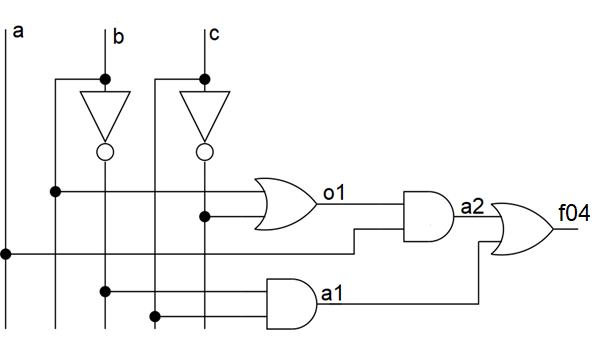
\includegraphics{image6.png}

\begin{enumerate}
\def\labelenumi{\arabic{enumi}.}
\item
  Create \textbf{a new project} folder within your \emph{lab1} directory
  called \emph{function04.}
\item
  Download \emph{function04.v} and \emph{function04}\_tb.v from Canvas
  to the project directory.
\item
  Create a project for these two files using the steps above.
\item
  \protect\hypertarget{Part_4_Step_4}{}{}Modify \emph{function04.v} by
  writing an assignment statement for each of \emph{o1}, \emph{a1},
  \emph{a2}, and \emph{f04}.
\item
  Modify \emph{function04\_tb.v} so that \emph{f04} is run through every
  combination of inputs. Assert the inputs in increasing binary
  numbering order starting from 0,0,0 and going to 1,1,1.
\item
  Perform simulation using this test bench as described in previous
  steps. You will need to ``run 100'' twice as the simulation is over
  100ns long.
\item
  \protect\hypertarget{Part_4_Step_7}{}{}Save this waveform as an image
  as done in a previous section. Color intermediate signals (01, a1, a2)
  yellow and output red.
\item
  \protect\hypertarget{Part_4_Step_8}{}{}From the information in the
  timing diagram, produce a truth table.
\end{enumerate}

\hypertarget{turn-in}{%
\section{Turn in:}
\label{turn-in}}

Make a record of your response to numbered items below and turn them in
a single copy as your team's solution on Canvas using the instructions
posted there. Include the names of both team members at the top of your
solutions. Use complete English sentences to introduce what each of the
following listed items (below) is and how it was derived.

\textbf{Part 1:} \protect\hyperlink{Part_1_Step_23}{Step 23} Timing
diagram of AND gate

\textbf{Part 2:} \protect\hyperlink{Part_2_Step_4}{Step 4} Verilog code
for \emph{f02}

\textbf{Part 2:} \protect\hyperlink{Part_2_Step_7}{Step 7} Timing
diagram of \emph{f02}

\textbf{Part 2:} \protect\hyperlink{Part_2_Step_8}{Step 8} Truth table
of \emph{f02}

\textbf{Part 3:} \protect\hyperlink{Part_3_Step_6}{Step 6} Timing
diagram of \emph{f03}

\textbf{Part 3:} \protect\hyperlink{Part_3_Step_7}{Step 7} Truth table
of \emph{f03}

\textbf{Part 3:} \protect\hyperlink{Part_3_Step_8}{Step 8} Circuit
Diagram of \emph{f03}

\textbf{Part 3:} \protect\hyperlink{Part_3_Step_9}{Step 9} Symbolic form
of \emph{f03}

\textbf{Part 4:} \protect\hyperlink{Part_4_Step_4}{Step 4} Just the 4
Verilog assign statement for \emph{o1}, \emph{a1}, \emph{a2}, and
\emph{f04}.

\textbf{Part 4:} \protect\hyperlink{Part_4_Step_7}{Step 7} Timing
diagram of \emph{f04}

\textbf{Part 4:} \protect\hyperlink{Part_4_Step_8}{Step 8} Truth table
of \emph{f04}



\chapter{Hexadecimal to Seven-Segment Converter}
\label{HexToSeven}
\graphicspath{ {./Lab02HexToSeven/Fig} }


\hypertarget{objective}{%
\section{\texorpdfstring{Objective }{Objective }}\label{objective}}

The objective of this lab is to become familiar with the always
statement used to implement truth tables, how to combine bits into
vectors and how to download synthesized code onto the development board.

Today's laboratory will require to learn about two new Verilog concepts,
The Always statement and Vectors. Let's look at the easier of these two,
Vectors, first.

\textbf{Vectors}

A vector is simply a collection of bits, very similar to an array in a
regular programming language. You might use a vector to represent a
3-bit binary number that you want to perform an operation on. There are
three things that you will need to know about vectors in order to
complete today's lab (and future labs), combining bits into a vector,
defining a vector, and accessing the bits of a vector. These operations
are illustrated in Figure 1.

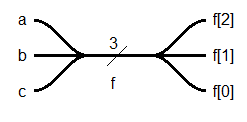
\includegraphics{image1.png}

Figure 1: A schematic illustration of combining bits into a vector, f,
and then accessing the individual bits of f.

Let's explore these ideas with the code snipped show in Figure 2. In
this code snipped, the line of code assign f = \{a,b,c\}; combines the
individual signals a, b and c into a 3-bit vector. The left-most signal
in the parenthesis list becomes the MSB of the vector and the right-most
becomes LSB. In other words, \emph{a} is the MSB and \emph{c} the LSB.
Combining signals is more commonly called concatenation. You can
concatenate any arrangement of signals as long as the number of bits
comes out the same as the signal on the left-hand-side of the = sign.

The statement wire {[}2:0{]} f; is how you define a vector. The numbers
in the square brackets are the indices of the most and least significant
bits of the vector. We will always index our vectors starting at 0, so
the highest index will always be one less than the number of elements in
the vector.

The statement assign x = (f{[}0{]} \& f{[}1{]}) \^{} f{[}2{]}; shows how
you can access the individual bits of a vector. While I am not sure what
the Verilog programmer was going for in this statement, you can access
the individual bit of a vector by putting the index of that bit in
square brackets. You can also access sub-vector by putting indices in
square brackets separated by a colon.

You can provide a constant value to a vector, an operation we will call
hardcoding, using the 3b'010; notation. The first number, 3, is the
length of the vector, b' means that this is a bit vector and the 010 is
the 3-bit value.

\textbf{Always}

We will use the Verilog \emph{always} statement to implement a function
using its truth table. Figure 3 shows an always statement that uses the
value of a signal x to compute the value of f.

For the time being, we will trust that the statement always @(*)allows
the code between case and endcase to run continuously and concurrent
with any other statements in the module. Yes, this means that all the
code between case and endcase acts like a single assign statement. A
case statement uses the argument to case (in this case x) as a selector
for one of the rows below. Every possible value of x must be present and
when that value matches x, the action to the right of the colon is
performed. When we use a case statement as shown in Figure 3 you must
make the output type reg.

All signals are either wire or reg type. A wire is a signal that has a
value provided to it by some active element. This active element might
be a gate or the output of a module. If a signal does not have an
explicit gate or module driving its value, it needs to be typed reg.

\hypertarget{part-1-combine-lab-1-functions.}{%
\section{Part 1: Combine lab 1
functions.}\label{part-1-combine-lab-1-functions.}}

Let's explore vectors and the always statement by combining the three
functions created in last weeks assignment into one function.

\begin{enumerate}
\def\labelenumi{\arabic{enumi}.}
\item
  Go back to your Lab 01 solutions and extract the truth tables for
  function f04, f03, and f02. Put these values into the truth table
  below.
\end{enumerate}

\begin{longtable}[]{@{}
  >{\raggedright\arraybackslash}p{(\columnwidth - 10\tabcolsep) * \real{0.1667}}|
  >{\raggedright\arraybackslash}p{(\columnwidth - 10\tabcolsep) * \real{0.1667}}|
  >{\raggedright\arraybackslash}p{(\columnwidth - 10\tabcolsep) * \real{0.1667}}|
  >{\raggedright\arraybackslash}p{(\columnwidth - 10\tabcolsep) * \real{0.1667}}|
  >{\raggedright\arraybackslash}p{(\columnwidth - 10\tabcolsep) * \real{0.1667}}|
  >{\raggedright\arraybackslash}p{(\columnwidth - 10\tabcolsep) * \real{0.1667}}@{}}
\caption{Table 1: The Truth Table for the combinedLab01 function. This
function has a 3-bit input and 3-bits output.}\tabularnewline
\toprule()
\begin{minipage}[b]{\linewidth}\raggedright
a
\end{minipage} & \begin{minipage}[b]{\linewidth}\raggedright
b
\end{minipage} & \begin{minipage}[b]{\linewidth}\raggedright
C
\end{minipage} & \begin{minipage}[b]{\linewidth}\raggedright
f04
\end{minipage} & \begin{minipage}[b]{\linewidth}\raggedright
f03
\end{minipage} & \begin{minipage}[b]{\linewidth}\raggedright
f02
\end{minipage} \\
\midrule()
\endfirsthead
\toprule()
\begin{minipage}[b]{\linewidth}\raggedright
a
\end{minipage} & \begin{minipage}[b]{\linewidth}\raggedright
b
\end{minipage} & \begin{minipage}[b]{\linewidth}\raggedright
C
\end{minipage} & \begin{minipage}[b]{\linewidth}\raggedright
f04
\end{minipage} & \begin{minipage}[b]{\linewidth}\raggedright
f03
\end{minipage} & \begin{minipage}[b]{\linewidth}\raggedright
f02
\end{minipage} \\ \hline
\midrule()
\endhead
0 & 0 & 0 & & & \\ \hline
0 & 0 & 1 & & & \\ \hline
0 & 1 & 0 & & & \\ \hline
0 & 1 & 1 & & & \\ \hline
1 & 0 & 0 & & & \\ \hline
1 & 0 & 1 & & & \\ \hline
1 & 1 & 0 & & & \\ \hline
1 & 1 & 1 & & & \\
\bottomrule()
\end{longtable}

\begin{enumerate}
\def\labelenumi{\arabic{enumi}.}
\item
  Create \textbf{a new project} folder within your \emph{lab2} directory
  called \emph{combinedLab01.}
\item
  Download \emph{combinedLab01.v} and \emph{combinedLab01}\_tb.v from
  Canvas to the project directory.
\item
  Create a project for these two files using the steps from last week's
  lab. For your convenience, these are given at the end of this document
  in the section entitled \textbf{Creating a Project}.
\item
  Modify \emph{combinedLab01.v} so that \emph{combinedLab01} outputs the
  values given in Table 1.
\item
  Modify \emph{combinedLab01\_tb.v} so that \emph{combinedLab01} is run
  through every combination of inputs. Assert the inputs in increasing
  binary numbering order starting from 0,0,0 and going to 1,1,1.
\item
  Perform simulation using this test bench using the steps from last
  week's lab. For your convenience, these are given at the end of this
  document in the section entitled \textbf{Performing a Simulation}.
\item
  \protect\hypertarget{CombinedLab01_Waveform}{}{}Capture the output
  waveform from Simulink. It should look something like the following.
\end{enumerate}

\begin{quote}
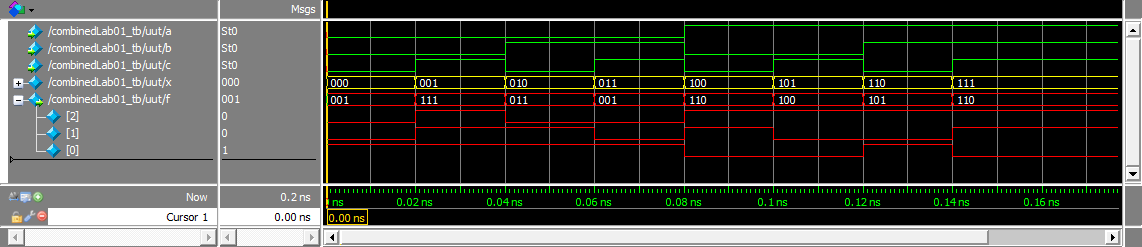
\includegraphics{image2.png}
\end{quote}

\begin{enumerate}
\def\labelenumi{\arabic{enumi}.}
\setcounter{enumi}{7}
\item
  From the information in the timing diagram, produce a truth table
  similar (exactly?) the same as Figure 4.
\end{enumerate}

\textbf{Bridging the divide between logical and physical}

The process of converting your Verilog code to a form which you will
download onto the development board is called \emph{synthesis}. In order
to synthesize your Verilog code, you need to tell the Quartus software
which pins of the FPGA are associated with the ports in your top-level
Verilog module. In order to perform this assignment, you need to know
which pins of the FPGA are associated with useful hardware on the
development board. The engineers who created the development board made
the assignment of hardware components to FPGA pins when they laid out
the printed circuit board. These same engineers documented their
decisions in the Cyclone V GX Kit User Manual posted on the class web
page.

The Figure 1 shows a Verilog module called \emph{combinedLab01}
synthesized and downloaded into an Altera FPGA on the development board.
Note that ports a, b and c are connected to FPGA pins that are driven to
slide switches. Ports f{[}2{]}, f{[}1{]} and f{[}0{]} are connected to
FPGA pins that drive LEDs. In this way, a user can provide input to the
\emph{combinedLab01} module by moving the slide switches and observe the
circuit's output on the LEDs.

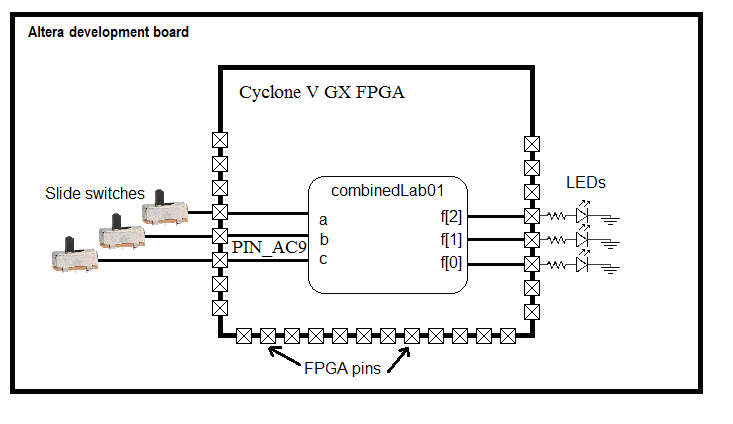
\includegraphics{image3.png}

Figure 5: A simple Verilog design synthezied and downloaded onto the
development board.

The development board contains an Altera Cyclone V GX FPGA. This FPGA
has many pins and they are identified by a lettered group and number.
For example, in Figure 1 port c of the combinedLab01 module is mapped to
pin AC9.

You will need to be able to figure out the remaining pin assignments on
your own. To do this open up the User Manual posted on the class Canvas
page. Go to page \textbf{32} of the User Manual and find Table 3-3. It
shows that slide switch SW{[}0{]} is connected to PIN\_AC9.

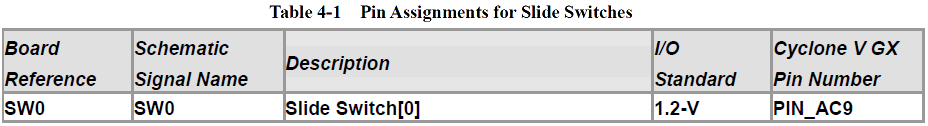
\includegraphics{image4.png}

The LEDs shown in figure 4-9 in the User Manual are active high, meaning
that the LED is active (illuminates) when you send it a high signal
(logic 1). Clearly, sending the LED a logic 0 turns the LED off. You can
place the slide switches in one of two positions (up or down). In the up
position, they assert a logic 1 on their input pin. Down causes the
slide switch to assert a logic 0 on its input pin.

Use the information to complete the following table. We will call this
the ``pin assignment table'' and use it in the next section.

\begin{longtable}[]{@{}
  >{\raggedright\arraybackslash}p{(\columnwidth - 12\tabcolsep) * \real{0.1429}}|
  >{\raggedright\arraybackslash}p{(\columnwidth - 12\tabcolsep) * \real{0.1428}}|
  >{\raggedright\arraybackslash}p{(\columnwidth - 12\tabcolsep) * \real{0.1428}}|
  >{\raggedright\arraybackslash}p{(\columnwidth - 12\tabcolsep) * \real{0.1428}}|
  >{\raggedright\arraybackslash}p{(\columnwidth - 12\tabcolsep) * \real{0.1429}}|
  >{\raggedright\arraybackslash}p{(\columnwidth - 12\tabcolsep) * \real{0.1430}}|
  >{\raggedright\arraybackslash}p{(\columnwidth - 12\tabcolsep) * \real{0.1430}}@{}}
\caption{\protect\hypertarget{CombinedLab01_Pin_assignment}{}{}Table 2:
Pin Assignment Table for combinedLab01.}\tabularnewline
\toprule()
\begin{minipage}[b]{\linewidth}\raggedright
Port
\end{minipage} & \begin{minipage}[b]{\linewidth}\raggedright
a
\end{minipage} & \begin{minipage}[b]{\linewidth}\raggedright
b
\end{minipage} & \begin{minipage}[b]{\linewidth}\raggedright
c
\end{minipage} & \begin{minipage}[b]{\linewidth}\raggedright
f{[}2{]}
\end{minipage} & \begin{minipage}[b]{\linewidth}\raggedright
f{[}1{]}
\end{minipage} & \begin{minipage}[b]{\linewidth}\raggedright
f{[}0{]}
\end{minipage} \\ \hline
\midrule()
\endfirsthead
\toprule()
\begin{minipage}[b]{\linewidth}\raggedright
Port
\end{minipage} & \begin{minipage}[b]{\linewidth}\raggedright
a
\end{minipage} & \begin{minipage}[b]{\linewidth}\raggedright
b
\end{minipage} & \begin{minipage}[b]{\linewidth}\raggedright
c
\end{minipage} & \begin{minipage}[b]{\linewidth}\raggedright
f{[}2{]}
\end{minipage} & \begin{minipage}[b]{\linewidth}\raggedright
f{[}1{]}
\end{minipage} & \begin{minipage}[b]{\linewidth}\raggedright
f{[}0{]}
\end{minipage} \\ \hline
\midrule()
\endhead
Signal name & SW{[}2{]} & SW{[}1{]} & SW{[}0{]} & LEDR{[}2{]} &
LEDR{[}1{]} & LEDR{[}0{]} \\
FPGA Pin No. & & & PIN\_AC9 & & & \\ \hline
\bottomrule()
\end{longtable}

\textbf{Synthesizing a Verilog Module}

It's time to realize the \emph{combinedLab01} Verilog file to FPGA. To
do this follow these steps:

\begin{enumerate}
\def\labelenumi{\arabic{enumi}.}
\item
  In Project Navigator pane, select the File tab
\item
  Right mouse click \emph{combinedLab01.v} and select Set As Top Level
  Entity.
\item
  Processing -\textgreater{} Start -\textgreater{} Start Analysis and
  Elaboration
\item
  Assignments -\textgreater{} Pin Planner
\item
  In the Pin Planner pop-up you should see the pin assignment pane at
  the bottom of the window.
\end{enumerate}

\begin{quote}
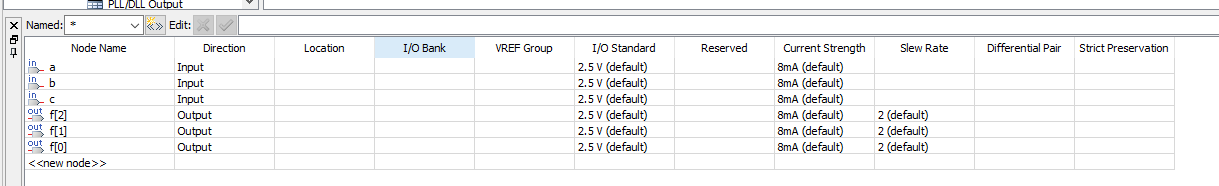
\includegraphics{image5.png}
\end{quote}

\begin{enumerate}
\def\labelenumi{\arabic{enumi}.}
\setcounter{enumi}{5}
\item
  Double click in the Location cell for row c
\item
  Scroll down the list of pins to PIN\_AC9
\item
  Complete the pin assignment for the other 5 inputs and outputs using
  the information contained in pin assignment table completed earlier.
\item
  Double check your pin assignments.
\item
  File -\textgreater{} Close. Note closing your file incorporates this
  assignment into the project.
\item
  Back in the Quartus window, Processing -\textgreater{} Start
  Compilation \textless Ctrl-L\textgreater{}
\item
  Tools -\textgreater{} Programmer
\item
  In the Programmer pop-up window click Add File\ldots{}
\item
  In the Select Programming File pop-up, navigate to your project
  directory, then into the output files folder, the select
  combinedLab01.sof, click Open. You should see something like the
  following.
\end{enumerate}

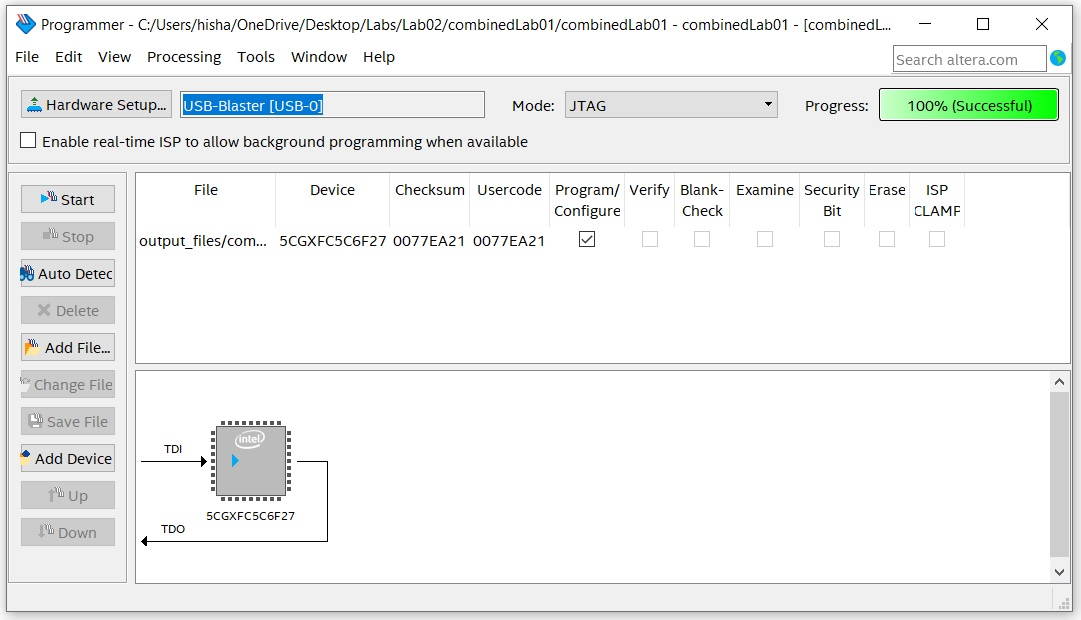
\includegraphics{image6.png}

\begin{enumerate}
\def\labelenumi{\arabic{enumi}.}
\setcounter{enumi}{14}
\item
  Connect the Altera Cyclone V GX FPGA to your computer through the USB
  port, connect the power supply, and push the red power-on button. Try
  not to be annoyed by the infernal blinking LEDs.
\item
  In the Programmer pop-up

  \begin{enumerate}
  \def\labelenumii{\alph{enumii}.}
  \item
    Click Hardware Setup\ldots.
  \item
    In the Hardware Setup select USB-Blaster {[}USB=0{]} from the
    Currently selected hardware pull-down
  \item
    Click Close
  \end{enumerate}
\item
  Back in the Programmer window, the box next to Hardware Setup\ldots{}
  should reflect your choice. Click Start,
\item
  The Development board should stop its infernal blinking and run your
  program. You may notice that the unused LEDs are dimly illuminated.
\end{enumerate}

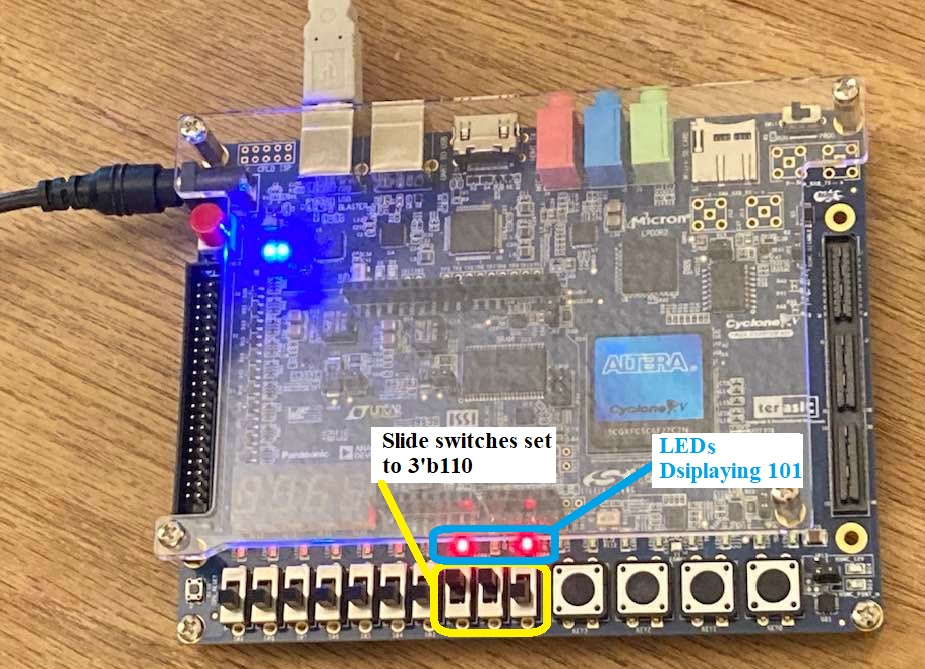
\includegraphics{image7.png}

Figure 6: The Development board properly configured and running the
combinedLab01 Verilog file.

\hypertarget{part-2-hexadecimal-to-7-segment-converter}{%
\section{Part 2: Hexadecimal to 7-segment
Converter}\label{part-2-hexadecimal-to-7-segment-converter}}

While working on the previous problem, you probably noticed that the
Development Board has four 7-segment display. These figure 8 shaped
blocks above the slide switches are the devices which light up numbers
on some cash registers. We will be using these 7-segment displays for a
variety of purposes during the term, so it would be a good idea.

The hexadecimal-to-seven-segment-decoder is a combinational circuit that
converts a hexadecimal number to an appropriate code that drives a
7-segment display the corresponding value. \uline{BEWARE, the LEDs in
the 7-segment displays on the Development Board are active low,
asserting a logic 0 on the pin attached to a segment will cause that
segment to illuminate.}

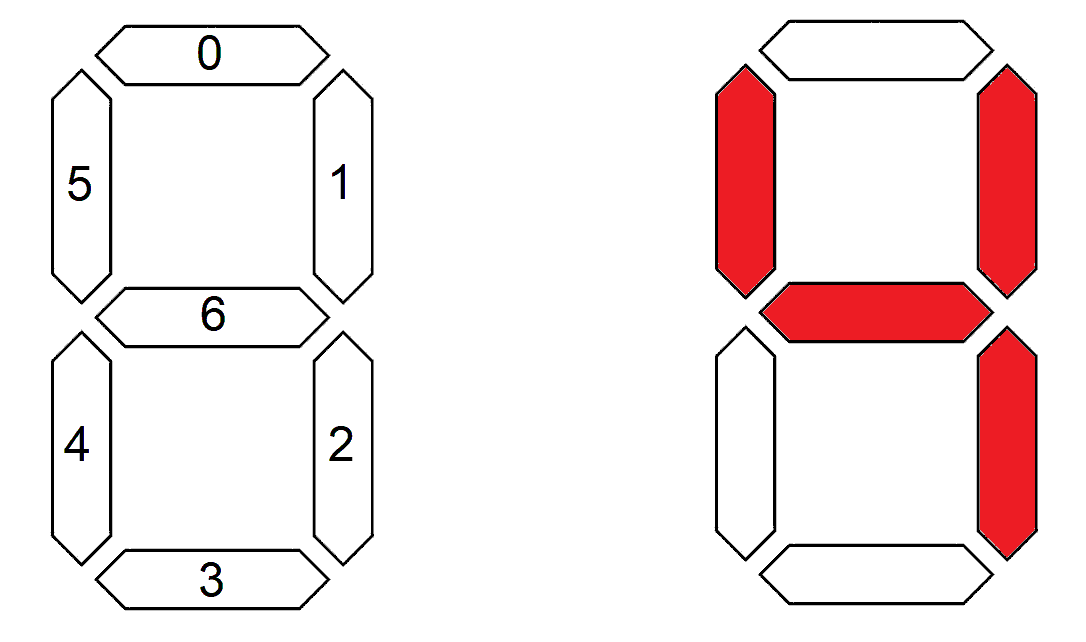
\includegraphics{image8.png}

Figure 7: Left, the proper numbering of the segments. Right,
illuminating segments to form the number 4.

The pattern of segments to be illuminated for each digit is shown in
Figure 7. For example, to display `4 output would be:

seg{[}6{]}=0 seg{[}5{]}=0 seg{[}4{]}=1 seg{[}3{]}=1 seg{[}2{]}=0
seg{[}1{]}=0 seg{[}0{]}=1

or seg = 7'b0011001

Figure 8 shows the proper formatting for all the values between 0 -- f.

\begin{quote}
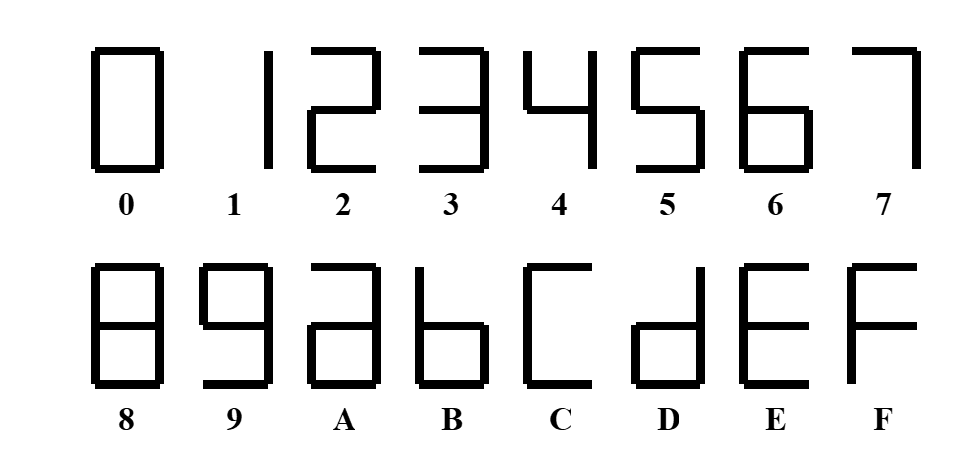
\includegraphics{image9.png}
\end{quote}

Figure 8: The proper arrangement of LEDs to form hexadecimal characters.

Figure 9 shows the Verilog module you will be building in this lab - a
circuit that converts a 4-bit input, representing a hexadecimal value,
into the binary values to illuminate a 7-segment display with active low
LEDs.

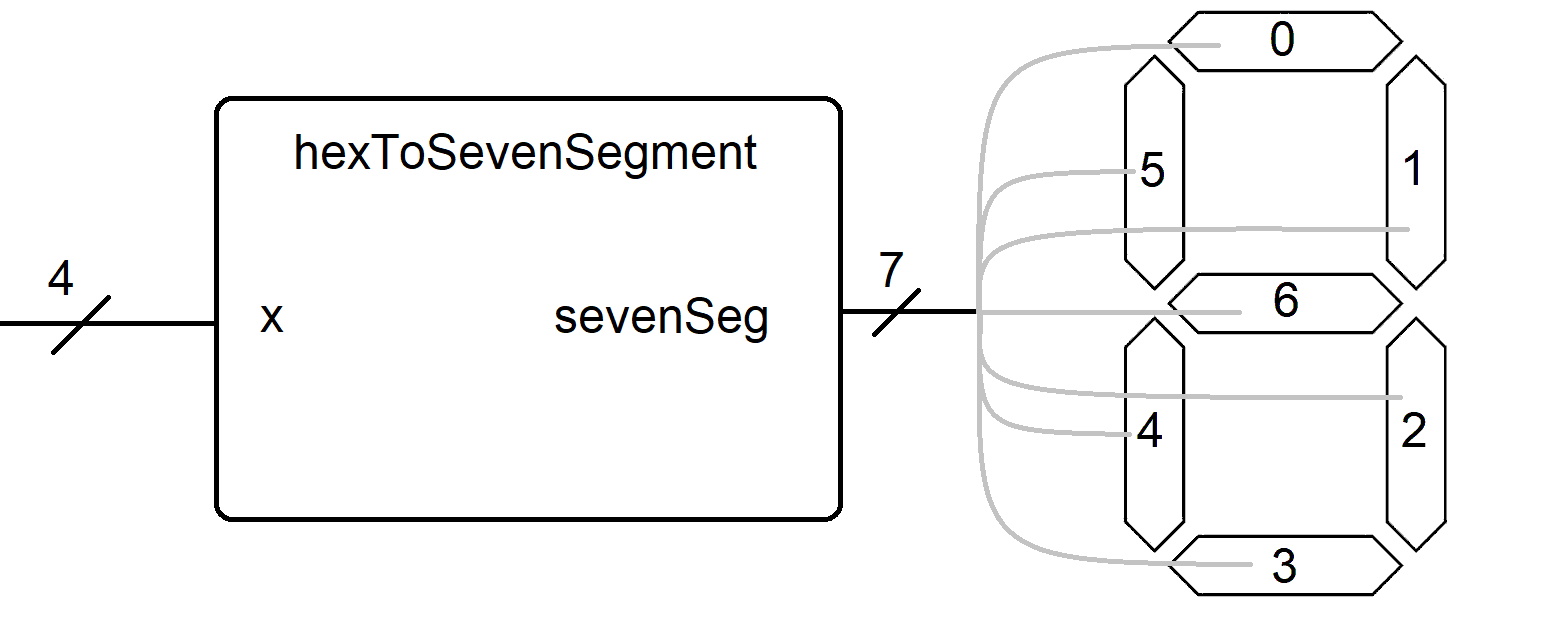
\includegraphics{image10.png}

Figure 9: The hexToSevenSeg Verilog module driving a 7-segment display.

\begin{enumerate}
\def\labelenumi{\arabic{enumi}.}
\item
  Complete the following table to illuminate the active low led segments
  to generate proper hexadecimal characters. I've renamed the sevenSeg
  output ``seg'' in the following table in order to make everything fit
  nicely.
\end{enumerate}

\begin{longtable}[]{@{}
  >{\raggedright\arraybackslash}p{(\columnwidth - 14\tabcolsep) * \real{0.1241}}|
  >{\raggedright\arraybackslash}p{(\columnwidth - 14\tabcolsep) * \real{0.1252}}|
  >{\raggedright\arraybackslash}p{(\columnwidth - 14\tabcolsep) * \real{0.1251}}|
  >{\raggedright\arraybackslash}p{(\columnwidth - 14\tabcolsep) * \real{0.1251}}|
  >{\raggedright\arraybackslash}p{(\columnwidth - 14\tabcolsep) * \real{0.1251}}|
  >{\raggedright\arraybackslash}p{(\columnwidth - 14\tabcolsep) * \real{0.1251}}|
  >{\raggedright\arraybackslash}p{(\columnwidth - 14\tabcolsep) * \real{0.1252}}|
  >{\raggedright\arraybackslash}p{(\columnwidth - 14\tabcolsep) * \real{0.1252}}@{}}
\caption{\protect\hypertarget{Hex2Seven_TruthTable}{}{}Table 3: Truth
table or the hexToSevenSeg component.}\tabularnewline
\toprule()
\begin{minipage}[b]{\linewidth}\raggedright
x
\end{minipage} & \begin{minipage}[b]{\linewidth}\raggedright
seg{[}6{]}
\end{minipage} & \begin{minipage}[b]{\linewidth}\raggedright
seg{[}5{]}
\end{minipage} & \begin{minipage}[b]{\linewidth}\raggedright
seg{[}4{]}
\end{minipage} & \begin{minipage}[b]{\linewidth}\raggedright
seg{[}3{]}
\end{minipage} & \begin{minipage}[b]{\linewidth}\raggedright
seg{[}2{]}
\end{minipage} & \begin{minipage}[b]{\linewidth}\raggedright
seg{[}1{]}
\end{minipage} & \begin{minipage}[b]{\linewidth}\raggedright
seg{[}0{]}
\end{minipage} \\ \hline
\midrule()
\endfirsthead
\toprule()
\begin{minipage}[b]{\linewidth}\raggedright
x
\end{minipage} & \begin{minipage}[b]{\linewidth}\raggedright
seg{[}6{]}
\end{minipage} & \begin{minipage}[b]{\linewidth}\raggedright
seg{[}5{]}
\end{minipage} & \begin{minipage}[b]{\linewidth}\raggedright
seg{[}4{]}
\end{minipage} & \begin{minipage}[b]{\linewidth}\raggedright
seg{[}3{]}
\end{minipage} & \begin{minipage}[b]{\linewidth}\raggedright
seg{[}2{]}
\end{minipage} & \begin{minipage}[b]{\linewidth}\raggedright
seg{[}1{]}
\end{minipage} & \begin{minipage}[b]{\linewidth}\raggedright
seg{[}0{]}
\end{minipage} \\ \hline
\midrule()
\endhead
0000 & & & & & & & \\ \hline
0001 & & & & & & & \\ \hline
0010 & & & & & & & \\ \hline
0011 & & & & & & & \\ \hline
0100 & 0 & 0 & 1 & 1 & 0 & 0 & 1 \\ \hline
0101 & & & & & & & \\ \hline
0110 & & & & & & & \\ \hline
0111 & & & & & & & \\ \hline
1000 & & & & & & & \\ \hline
1001 & & & & & & & \\ \hline
1010 & & & & & & & \\ \hline
1011 & & & & & & & \\ \hline
1100 & & & & & & & \\ \hline
1101 & & & & & & & \\ \hline
1110 & & & & & & & \\ \hline
1111 & & & & & & & \\
\bottomrule()
\end{longtable}

Complete the pin assignment tables for the inputs and outputs

\begin{longtable}[]{@{}
  >{\raggedright\arraybackslash}p{(\columnwidth - 8\tabcolsep) * \real{0.1999}}|
  >{\raggedright\arraybackslash}p{(\columnwidth - 8\tabcolsep) * \real{0.1999}}|
  >{\raggedright\arraybackslash}p{(\columnwidth - 8\tabcolsep) * \real{0.2001}}|
  >{\raggedright\arraybackslash}p{(\columnwidth - 8\tabcolsep) * \real{0.1999}}|
  >{\raggedright\arraybackslash}p{(\columnwidth - 8\tabcolsep) * \real{0.2001}}@{}}
\caption{\protect\hypertarget{Hex2Seven_PinAssignment}{}{}Table 4: Pair
of pin assignment tables for the hexToSevenSeg
component.}\tabularnewline
\toprule()
\begin{minipage}[b]{\linewidth}\raggedright
Port
\end{minipage} & \begin{minipage}[b]{\linewidth}\raggedright
x{[}3{]}
\end{minipage} & \begin{minipage}[b]{\linewidth}\raggedright
x{[}2{]}
\end{minipage} & \begin{minipage}[b]{\linewidth}\raggedright
x{[}1{]}
\end{minipage} & \begin{minipage}[b]{\linewidth}\raggedright
x{[}0{]}
\end{minipage} \\ \hline
\midrule()
\endfirsthead
\toprule()
\begin{minipage}[b]{\linewidth}\raggedright
Port
\end{minipage} & \begin{minipage}[b]{\linewidth}\raggedright
x{[}3{]}
\end{minipage} & \begin{minipage}[b]{\linewidth}\raggedright
x{[}2{]}
\end{minipage} & \begin{minipage}[b]{\linewidth}\raggedright
x{[}1{]}
\end{minipage} & \begin{minipage}[b]{\linewidth}\raggedright
x{[}0{]}
\end{minipage} \\ \hline
\midrule()
\endhead
Signal name & SW{[}3{]} & SW{[}2{]} & SW{[}1{]} & SW{[}0{]} \\ \hline
FPGA Pin No. & & & & PIN\_AC9 \\
\bottomrule()
\end{longtable}

\begin{longtable}[]{@{}
  >{\raggedright\arraybackslash}p{(\columnwidth - 14\tabcolsep) * \real{0.1083}}|
  >{\raggedright\arraybackslash}p{(\columnwidth - 14\tabcolsep) * \real{0.1431}}|
  >{\raggedright\arraybackslash}p{(\columnwidth - 14\tabcolsep) * \real{0.1431}}|
  >{\raggedright\arraybackslash}p{(\columnwidth - 14\tabcolsep) * \real{0.1431}}|
  >{\raggedright\arraybackslash}p{(\columnwidth - 14\tabcolsep) * \real{0.1341}}|
  >{\raggedright\arraybackslash}p{(\columnwidth - 14\tabcolsep) * \real{0.1095}}|
  >{\raggedright\arraybackslash}p{(\columnwidth - 14\tabcolsep) * \real{0.1095}}|
  >{\raggedright\arraybackslash}p{(\columnwidth - 14\tabcolsep) * \real{0.1095}}@{}}
\toprule()
\begin{minipage}[b]{\linewidth}\raggedright
Port
\end{minipage} & \begin{minipage}[b]{\linewidth}\raggedright
sevenSeg{[}6{]}
\end{minipage} & \begin{minipage}[b]{\linewidth}\raggedright
sevenSeg{[}5{]}
\end{minipage} & \begin{minipage}[b]{\linewidth}\raggedright
sevenSeg{[}4{]}
\end{minipage} & \begin{minipage}[b]{\linewidth}\raggedright
sevenSeg{[}3{]}
\end{minipage} & \begin{minipage}[b]{\linewidth}\raggedright
sevenSeg{[}2{]}
\end{minipage} & \begin{minipage}[b]{\linewidth}\raggedright
sevenSeg{[}1{]}
\end{minipage} & \begin{minipage}[b]{\linewidth}\raggedright
sevenSeg{[}0{]}
\end{minipage} \\ \hline
\midrule()
\endhead
Signal name & HEX0{[}6{]} & HEX0{[}5{]} & HEX0{[}4{]} & HEX0{[}3{]} &
HEX0{[}2{]} & HEX0{[}1{]} & HEX0{[}0{]} \\ \hline
FPGA Pin No. & & & & & & & \\ \hline
\bottomrule()
\end{longtable}

\begin{enumerate}
\def\labelenumi{\arabic{enumi}.}
\setcounter{enumi}{1}
\item
  Create \textbf{a new project} folder within your \emph{lab2} directory
  called \emph{hexToSevenSeg.}
\item
  Download \emph{hexToSevenSeg.v} and \emph{hexToSevenSeg \_tb.v} from
  Canvas to the project directory.
\item
  Create a project for these two files.
\item
  \protect\hypertarget{Hex2Seven_Verilog}{}{}Complete the case statement
  for \emph{hexToSevenSeg.v}
\item
  Modify \emph{hexToSevenSeg \_tb.v} so that \emph{hexToSevenSeg} is run
  through every combination of inputs. Assert the inputs in increasing
  binary numbering order starting from 0,0,0,0 and going to 1,1,1,1.
\item
  Perform simulation using this test bench as described in previous
  steps. You will need to ``run 100'' several times to go through all
  the inputs.
\item
  \protect\hypertarget{Hex2Seven_Waveform}{}{}Save this waveform as an
  image as done in the previous section. If the waveform is missing, you
  can add it back in using View -\textgreater{} Waveform.
\item
  From the information in the timing diagram, produce a truth table for
  \emph{hexToSevenSeg}.
\item
  Synthesize your design, bask in the glow of another success.
\end{enumerate}

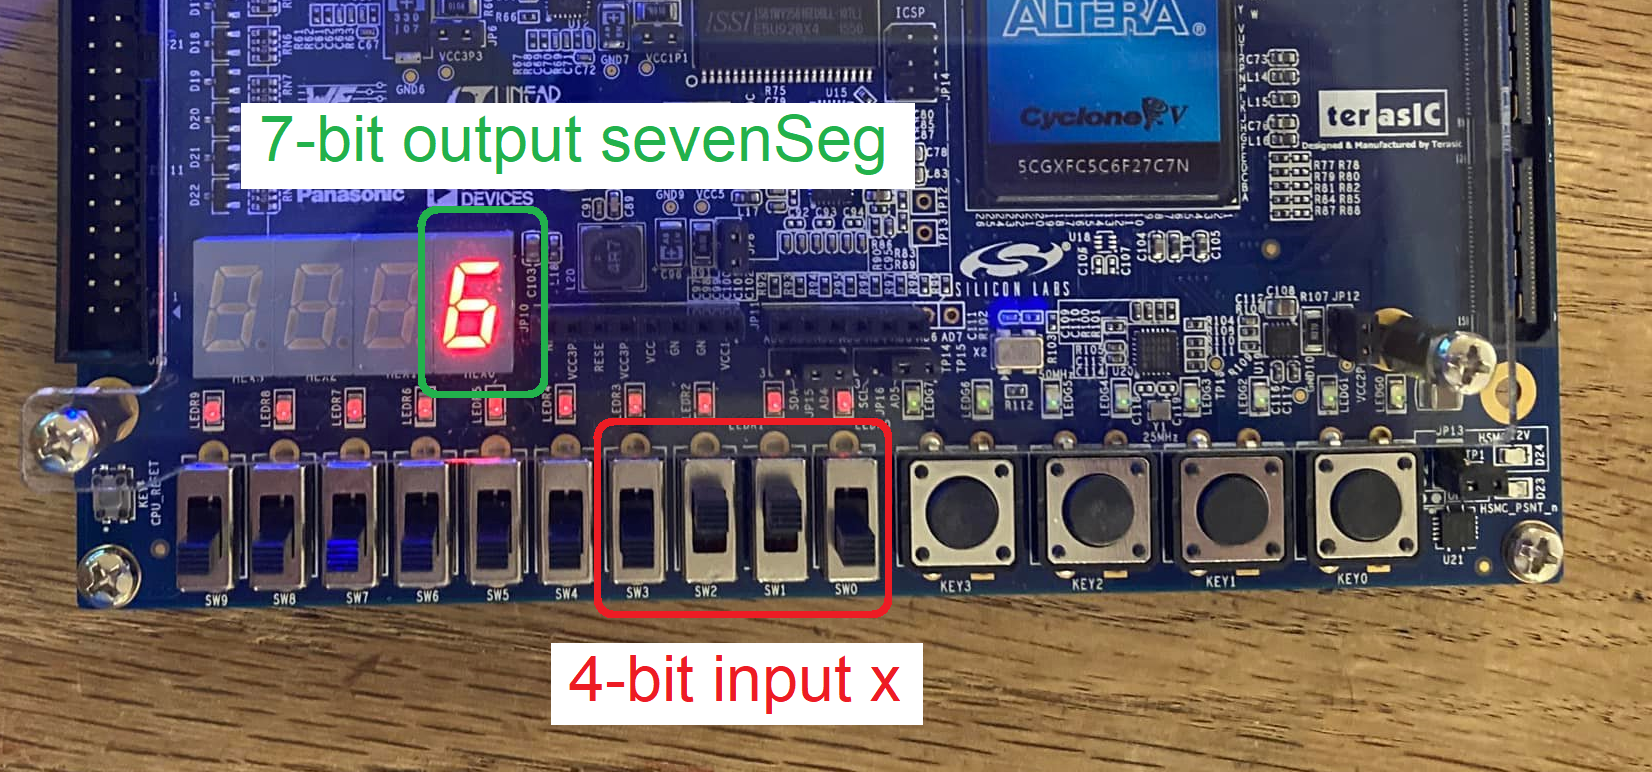
\includegraphics{image11.png}

\hypertarget{turn-in}{%
\section{Turn in:}\label{turn-in}}

Make a record of your response to numbered items below and turn them in
a single copy as your team's solution on Canvas using the instructions
posted there. Include the names of both team members at the top of your
solutions. Use complete English sentences to introduce what each of the
following listed items (below) is and how it was derived.

\textbf{Part 1:} \protect\hyperlink{CombinedLab01_Waveform}{Truth Table
for combinedLab01 function} (Table 1)

\protect\hyperlink{CombinedLab01_Waveform}{Timing diagram for
combinedLab01 function}

\protect\hyperlink{CombinedLab01_Pin_assignment}{Pin assignment for
combinedLab01} (Table 2)

\textbf{Part 2:} \protect\hyperlink{Hex2Seven_TruthTable}{Truth Table
for hexToSevenSeg function} (Table 3)

\protect\hyperlink{Hex2Seven_Verilog}{Verilog code for hexToSevenSeg
function} -- just the always/case statement

\protect\hyperlink{Hex2Seven_Waveform}{Timing diagram for hexToSevenSeg
function}

\protect\hyperlink{Hex2Seven_PinAssignment}{Pin assignment tables for
hexToSevenSeg} (Tables 4)

Demonstrate operation in lab



\chapter{Rock Paper Scissors}
\label{RPS}
\graphicspath{ {./Lab03RockPaperScissor/Fig} }


\hypertarget{objective}{%
\section{Objective }
\label{section:rpsObjective}}

The objective of this lab is to use the concepts learned to build a
digital system to play a game of rock, paper, scissors.

\subsubsection{Rock Paper, Scissors}

The game of rock, paper, scissors is a two-player game whose goal is to
beat the throw of the opposing player. Traditionally, each player throws
one of three plays, rock, paper, or scissors by extending their hand in
the shape of the object.

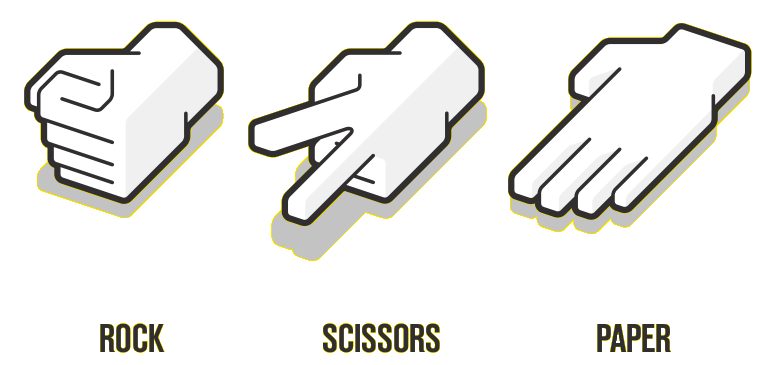
\includegraphics{ image1.png}

The rules of the game state that:

\begin{tabular}{p{4cm}p{4cm}p{4cm}}
Rock beats scissors  & Scissors beats paper & Paper beats rock \\
\end{tabular}

Since prior knowledge of your opponent's throw would provide an unfair
advantage, the two players make their throws at the same time. You goal 
in this lab is to create a digital version of rock, paper,
scissors using the Altera Cyclone V Board using the inputs and outputs
shown in Figure~\ref{figure:systemIO}. Each player will have access to three slide switches
and one 7-segment display. Each of the three switches represents one of
the three plays and the 7-segment will display the throw when the Play
button is pressed. The Win/Lose 7-segment display will show ``1'' when
player 1 wins, ``2'' when player 2 wins, and ``d'' when the game is a
draw (a tie).

\begin{figure}[ht]
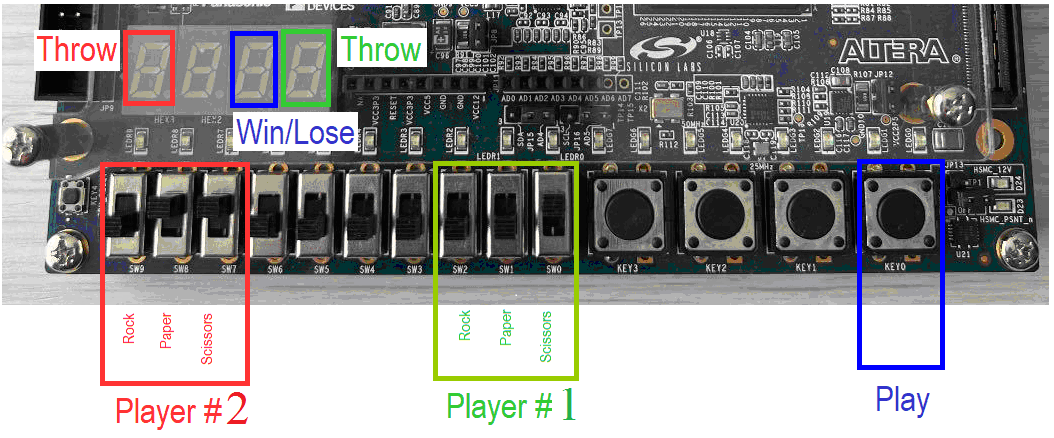
\includegraphics{ image2.png}
\caption{The input and output you should use to realize your digital system.}
\label{figure:systemIO}
\end{figure}



A player will move one of the three slides-switches into the up position
to indicate their play. Moving more than one slide-switch, or no slide
switch into the up position is in an invalid play. An invalid play
always loses to a valid play. If each player throws an invalid play, the
game is a draw.

While each player is making their choice of play, their Throw 7-segment
display will reflect their choice as shown in Figure~\ref{figure:play7seg}. These patterns
are supposed to vaguely resemble the objects.

\begin{figure}[ht]
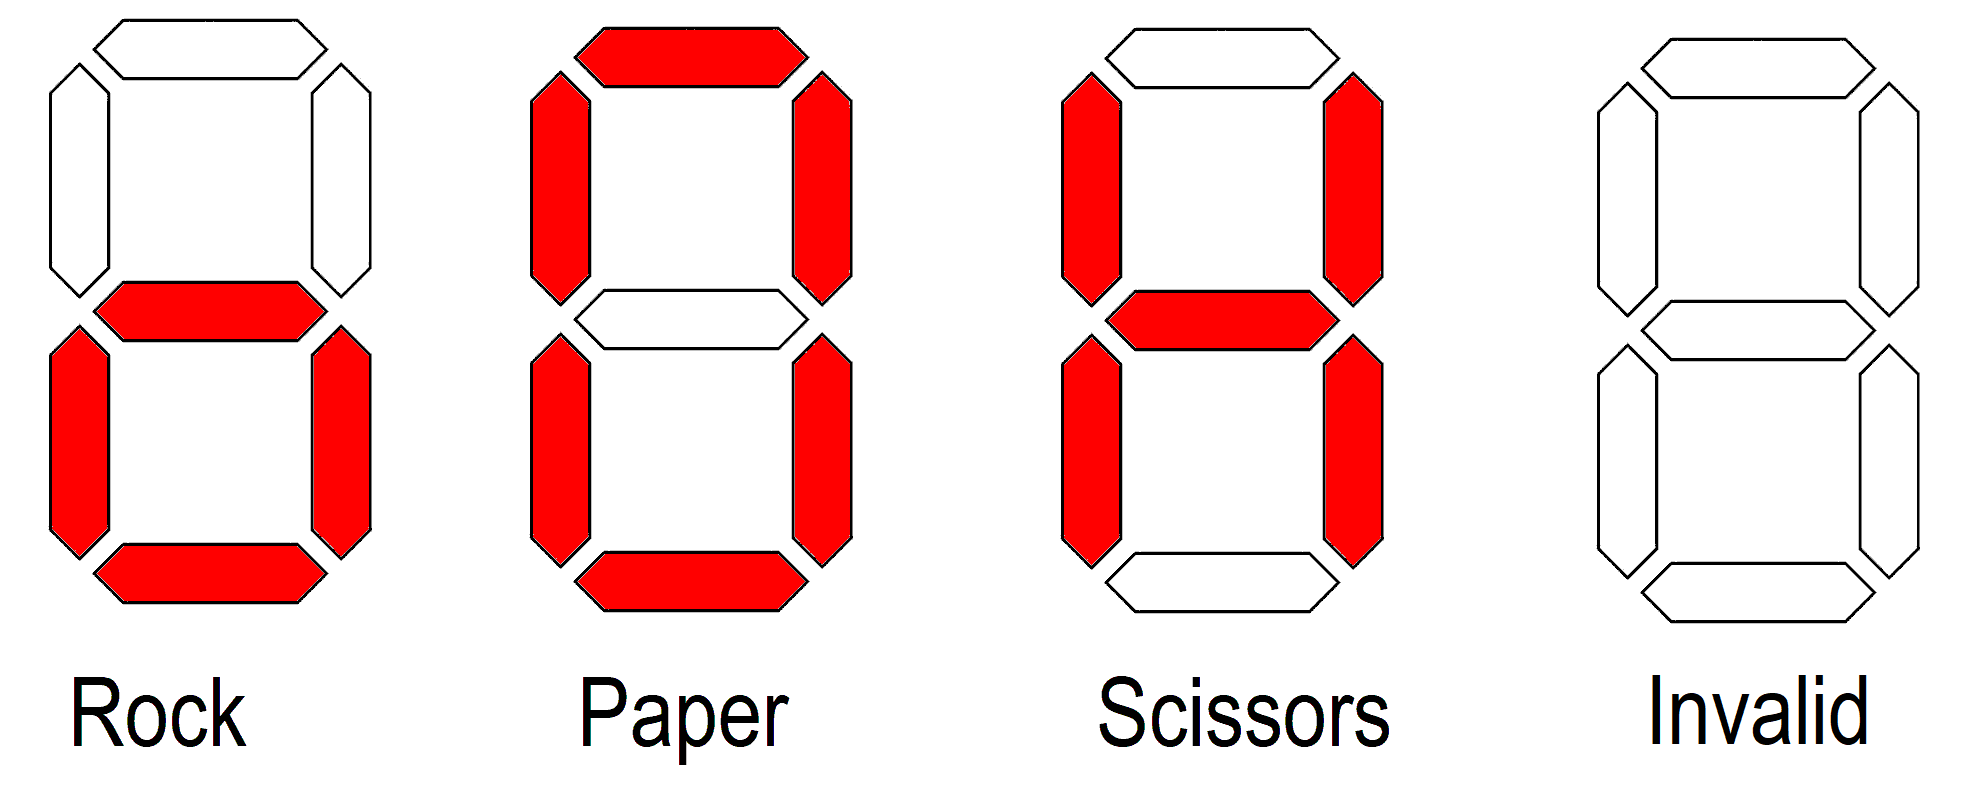
\includegraphics[width=0.5\paperwidth]{image3.png}
\caption{Illuminated patters for the different plays.}
\label{figure:play7seg}
\end{figure}

When the Throw button is pressed, the Win/Lose 7-segment will display
``1'', ``2'', or ``d'' depending on the outcome of the game as shown in
Table~\ref{table:gameLogic}. When the Throw button is un-pressed, the Win/Lose 7-segment
display is blank.

\begin{longtable}[]{@{}
  >{\raggedright\arraybackslash}p{(\columnwidth - 8\tabcolsep) * \real{0.1999}}|
  >{\raggedright\arraybackslash}p{(\columnwidth - 8\tabcolsep) * \real{0.2000}}|
  >{\raggedright\arraybackslash}p{(\columnwidth - 8\tabcolsep) * \real{0.2000}}|
  >{\raggedright\arraybackslash}p{(\columnwidth - 8\tabcolsep) * \real{0.2000}}|
  >{\raggedright\arraybackslash}p{(\columnwidth - 8\tabcolsep) * \real{0.2000}}@{}}
\caption{The output for every combination of player 1 (P1) and player 2 (P2) throws.}  
\label{table:gameLogic}
\tabularnewline
\toprule()
\begin{minipage}[b]{\linewidth}\raggedright
P1 \textbackslash{} P2
\end{minipage} & \begin{minipage}[b]{\linewidth}\raggedright
Rock
\end{minipage} & \begin{minipage}[b]{\linewidth}\raggedright
Paper
\end{minipage} & \begin{minipage}[b]{\linewidth}\raggedright
Scissors
\end{minipage} & \begin{minipage}[b]{\linewidth}\raggedright
Invalid
\end{minipage} \\ \hline
\midrule()
\endfirsthead
\toprule()
\begin{minipage}[b]{\linewidth}\raggedright
P1 \textbackslash{} P2
\end{minipage} & \begin{minipage}[b]{\linewidth}\raggedright
Rock
\end{minipage} & \begin{minipage}[b]{\linewidth}\raggedright
Paper
\end{minipage} & \begin{minipage}[b]{\linewidth}\raggedright
Scissors
\end{minipage} & \begin{minipage}[b]{\linewidth}\raggedright
Invalid
\end{minipage} \\\hline
\midrule()
\endhead
Rock & d & 2 & 1 & 1 \\ \hline
Paper & 1 & d & 2 & 1 \\ \hline
Scissors & 2 & 1 & d & 1 \\ \hline
Invalid & 2 & 2 & 2 & d \\

\end{longtable}

\textbf{System design}

There are an almost unlimited number of ways that you could implement
this digital system. Since this is your first lab building a system, you
must use the system architecture shown in Figure~\ref{fig:sysArch}. The names outside
the FPGA square correspond to the labels in Figure~\ref{figure:systemIO}. Each soft-square
(a square with rounded corners) is a Verilog module. Names inside
soft-squares, that are adjacent to lines outside the soft-square, are
the port names for that module. The instance name and module name of a
module are separated by a ``:'' and usually located along the top edge
of the soft-square. Red soft-squares are associated with player 1 and
green soft-squares associated with player 2. The names on lines inside
the rpsGame soft-square are the signals names you should use in the
rpsGame module to connect the 5 modules together. Lines that are slashed
with a number denote bit vectors.

\begin{figure}[ht]
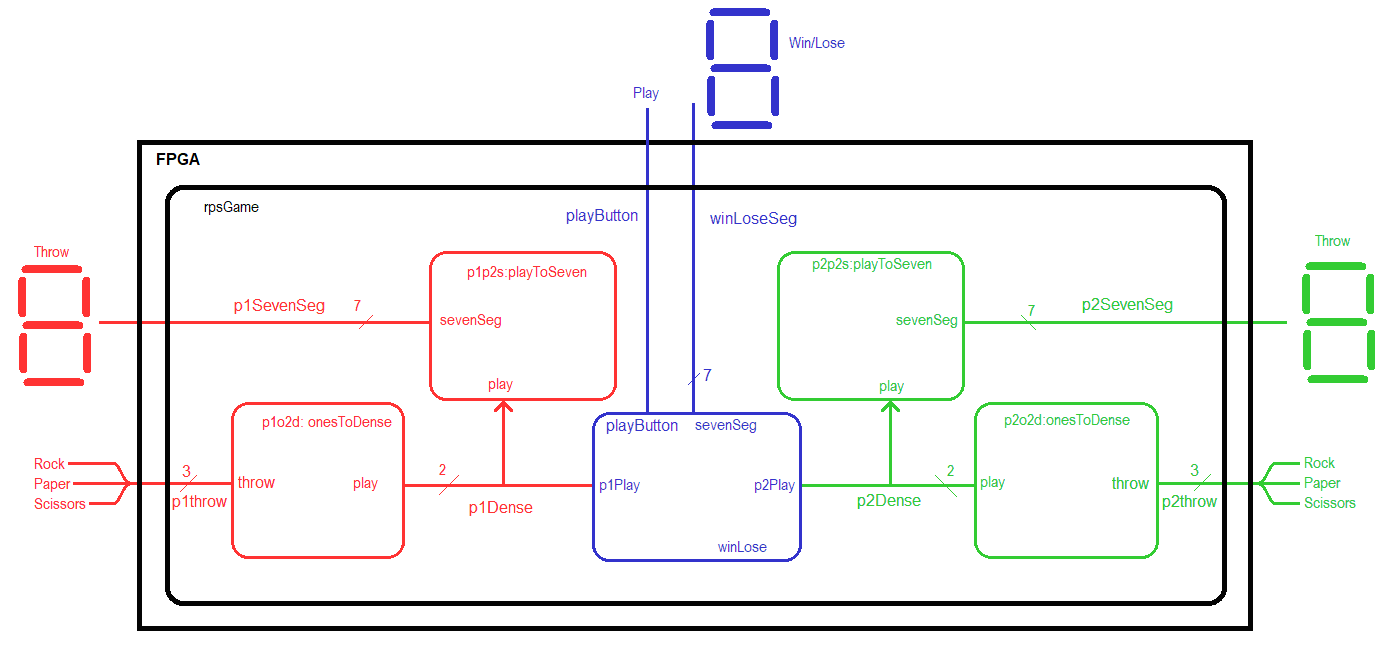
\includegraphics{ image4.png}
\caption{System architecture for the rock, paper, scissors system.}
\label{fig:sysArch}
\end{figure}

\hypertarget{onestodense-module}{%
\section{Module: onesToDense}
\label{onestodense-module}}

Each player makes their throw selection by placing one of the three
slide switches into the up position. As a result of this game mechanic,
there are only three valid input combinations for the rock, paper,
scissors trio. These are:

\begin{itemize}
\item
  (1,0,0) for when the player moves only the rock slide switch up,
\item
  (0,1,0) for when the player moves only the paper slide switch up,
\item
  (0,0,1) for when the player moves only the scissor slide switch up.
\end{itemize}

Having a code where only one of the bits is equal logic 1 is called a
``ones-hot'' code. The ``hot'' bit being logic 1. A code where every
possible combination of bits is assigned a meaning is called a dense
code.

This module will convert the input ones-hot code into a dense code. In
order to correctly determine the outcome of the game, we need to know
when the user has entered an invalid play; the output of this module
must be able to represent \{rock, paper, scissors, invalid\}. You will
encode these four combinations in 2-bits as \{2'b00, 2b'01, 2'b10,
2'b11\} respectively.

In order to write the Verilog code for this module, complete the truth
table in Table~\ref{table:onesToDense} for the onesToDense function.

\begin{itemize}
\item
  r is the state of the rock slide-switch. r=0 slide switch is down. r=1
  slide-switch up.
\item
  p is the state of the paper slide-switch. p=0 slide switch is down.
  p=1 slide-switch up
\item
  s is the state of the scissor slide-switch. s=0 slide switch is down.
  s=1 slide-switch up
\item
  play = \{00\} means rock was selected
\item
  play = \{01\} means paper was selected
\item
  play = \{10\} means scissor was selected
\item
  play = \{11\} means invalid selection was made
\end{itemize}

\begin{longtable}[]{@{}
  >{\raggedright\arraybackslash}p{(\columnwidth - 8\tabcolsep) * \real{0.1999}}|
  >{\raggedright\arraybackslash}p{(\columnwidth - 8\tabcolsep) * \real{0.2000}}|
  >{\raggedright\arraybackslash}p{(\columnwidth - 8\tabcolsep) * \real{0.2000}}|
  >{\raggedright\arraybackslash}p{(\columnwidth - 8\tabcolsep) * \real{0.2000}}|
  >{\raggedright\arraybackslash}p{(\columnwidth - 8\tabcolsep) * \real{0.2000}}@{}}
\caption{\protect\hypertarget{_Ref30701520}{}{}The truth table for the onesToDense function.}\\
\toprule()
\begin{minipage}[b]{\linewidth}\raggedright
r
\end{minipage} & \begin{minipage}[b]{\linewidth}\raggedright
p
\end{minipage} & \begin{minipage}[b]{\linewidth}\raggedright
s
\end{minipage} & \begin{minipage}[b]{\linewidth}\raggedright
play
\end{minipage} & \begin{minipage}[b]{\linewidth}\raggedright
Note
\end{minipage} \\ \hline
\midrule()
\endfirsthead
\toprule()
\begin{minipage}[b]{\linewidth}\raggedright
r
\end{minipage} & \begin{minipage}[b]{\linewidth}\raggedright
p
\end{minipage} & \begin{minipage}[b]{\linewidth}\raggedright
s
\end{minipage} & \begin{minipage}[b]{\linewidth}\raggedright
play
\end{minipage} & \begin{minipage}[b]{\linewidth}\raggedright
Note
\end{minipage} \\ \hline
\midrule()
\endhead
0 & 0 & 0 & & \\ \hline
0 & 0 & 1 & & \\ \hline
0 & 1 & 0 & & \\ \hline
0 & 1 & 1 & & \\ \hline
1 & 0 & 0 & 00 & Rock \\ \hline
1 & 0 & 1 & & \\ \hline
1 & 1 & 0 & & \\ \hline
1 & 1 & 1 & & \\
\label{table:onesToDense}
\end{longtable}

From this truth table, determine the canonical SOP expressions for
play{[}1{]} and play{[}0{]} functions. Do this by writing the canonical
SOP expression for the most significant bit of the play output,
play{[}1{]}, in the Table~\ref{table:onesToDense} truth table while ignoring the LSB. Then
proceed to write the canonical SOP expression for the LSB of the play
output, play{[}0{]}, in the Table~\ref{table:onesToDense} truth table while ignoring the MSB.

\protect\hypertarget{ones2Dense_CanonicalSOP}{}{}play{[}1{]} =

play{[}0{]} =

\protect\hypertarget{ones2Dense_Verilog}{}{}Now it's time to write the
Verilog code. Incorporate the following into your onesToDense Verilog
module:

\begin{itemize}
\item
  Use the module declaration: module onesToDense (throw, play);
\item
  Use vectors for the throw input. The MSB should come from the rock
  slide-switch and the LSB from the scissors slide-switch.
\item
  Use a vector for the play output.
\item
  Make the input and output port types ``wire''.
\item
  You may want to break the input vector into its component pieces to
  correspond to the variable names used in your kmap. This will require
  a wire declaration and two assign statements to give each variable
  1-bit from the input vector.
\item
  Use assign statements to realize the AND, OR, NOT logic derived for
  your canonical SOP expressions.
\item
  Use function04 from lab 1 as a starting point for this module.
\end{itemize}

\hypertarget{playtoseven-module}{%
\section{Module: playToSeven}
\label{playtoseven-module}}

The playToSeven module converts the player throw, represented in the
dense coding, to a ``graphical'' form displayed on the 7-segment
display. The symbols for each possible throw are shown in Figure~\ref{figure:throw7seg}.

\begin{figure}[ht]
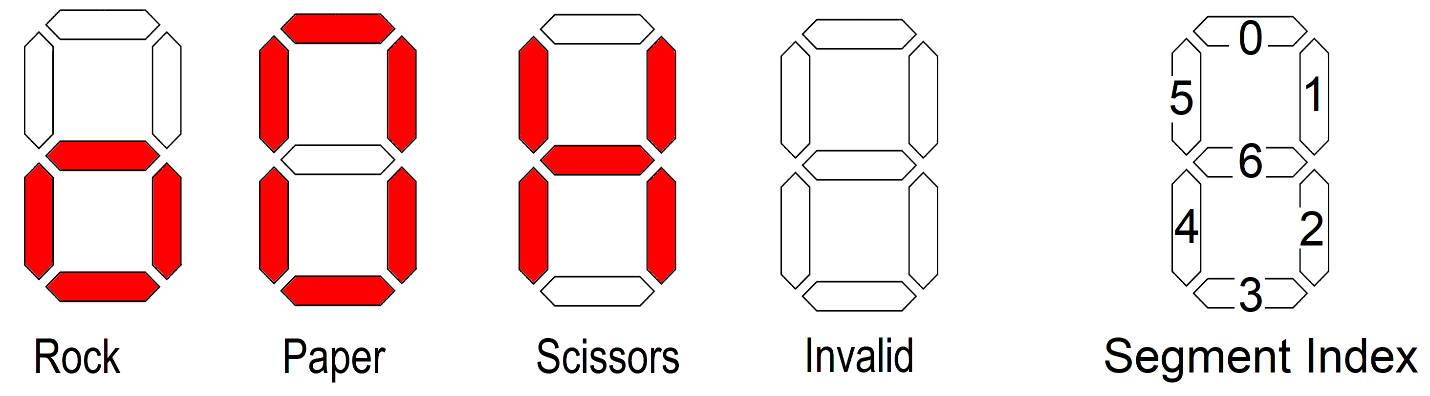
\includegraphics{ image5.png}
\caption{7-segment display patterns for the different throws along with
the 7-segment display segment indices.}
\label{figure:throw7seg}
\end{figure}

Use the information in Figure~\ref{figure:throw7seg} to determine the bit patterns needed to
generate the four different symbols in Table~\ref{table:throwSevenSeg}. Remember that the LEDs
in the segments are active low, meaning that a logic 0 output
illuminates an LED segment. In Table~\ref{table:throwSevenSeg} put a 0 or 1 in each of the
numbered column so that each row produces the patterns for its throw.
Remember that rock is coded as 00, paper as 01, scissors as 10 and an
invalid throw is coded as 11. In the sevenSeg column put the 7-bit code
formed by concatenating the bits together. Use proper Verilog syntax to
write this 7-bit vector.

\begin{longtable}[]{@{}
  >{\raggedright\arraybackslash}p{(\columnwidth - 18\tabcolsep) * \real{0.1513}}|
  >{\raggedright\arraybackslash}p{(\columnwidth - 18\tabcolsep) * \real{0.0643}}|
  >{\raggedright\arraybackslash}p{(\columnwidth - 18\tabcolsep) * \real{0.0643}}|
  >{\raggedright\arraybackslash}p{(\columnwidth - 18\tabcolsep) * \real{0.0643}}|
  >{\raggedright\arraybackslash}p{(\columnwidth - 18\tabcolsep) * \real{0.0643}}|
  >{\raggedright\arraybackslash}p{(\columnwidth - 18\tabcolsep) * \real{0.0643}}|
  >{\raggedright\arraybackslash}p{(\columnwidth - 18\tabcolsep) * \real{0.0643}}|
  >{\raggedright\arraybackslash}p{(\columnwidth - 18\tabcolsep) * \real{0.0643}}|
  >{\raggedright\arraybackslash}p{(\columnwidth - 18\tabcolsep) * \real{0.2210}}|
  >{\raggedright\arraybackslash}p{(\columnwidth - 18\tabcolsep) * \real{0.1777}}@{}}
\caption{\protect\hypertarget{_Ref30701476}{}{}Table to
determine the bit values for the 7-segment display LEDs to produce the
throw patterns.}\tabularnewline
\toprule()
\begin{minipage}[b]{\linewidth}\raggedright
pPlay
\end{minipage} & \begin{minipage}[b]{\linewidth}\raggedright
6
\end{minipage} & \begin{minipage}[b]{\linewidth}\raggedright
5
\end{minipage} & \begin{minipage}[b]{\linewidth}\raggedright
4
\end{minipage} & \begin{minipage}[b]{\linewidth}\raggedright
3
\end{minipage} & \begin{minipage}[b]{\linewidth}\raggedright
2
\end{minipage} & \begin{minipage}[b]{\linewidth}\raggedright
1
\end{minipage} & \begin{minipage}[b]{\linewidth}\raggedright
0
\end{minipage} & \begin{minipage}[b]{\linewidth}\raggedright
sevenSeg
\end{minipage} & \begin{minipage}[b]{\linewidth}\raggedright
Note
\end{minipage} \\
\midrule()
\endfirsthead
\toprule()
\begin{minipage}[b]{\linewidth}\raggedright
pPlay
\end{minipage} & \begin{minipage}[b]{\linewidth}\raggedright
6
\end{minipage} & \begin{minipage}[b]{\linewidth}\raggedright
5
\end{minipage} & \begin{minipage}[b]{\linewidth}\raggedright
4
\end{minipage} & \begin{minipage}[b]{\linewidth}\raggedright
3
\end{minipage} & \begin{minipage}[b]{\linewidth}\raggedright
2
\end{minipage} & \begin{minipage}[b]{\linewidth}\raggedright
1
\end{minipage} & \begin{minipage}[b]{\linewidth}\raggedright
0
\end{minipage} & \begin{minipage}[b]{\linewidth}\raggedright
sevenSeg
\end{minipage} & \begin{minipage}[b]{\linewidth}\raggedright
Note
\end{minipage} \\ \hline
\midrule()
\endhead
00 & & & & & & & & & Rock \\ \hline
01 & & & & & & & & & Paper \\ \hline
10 & & & & & & & & & Scissors \\ \hline
11 & & & & & & & & 7'b1111111 & Invalid \\
\bottomrule()
\label{table:throwSevenSeg}
\end{longtable}

\protect\hypertarget{play2Seven_Verilog}{}{}Incorporate the following
into your playToSeven Verilog module:

\begin{itemize}
\item
  Use the module declaration: \verb+module playToSeven (pPlay, sevenSeg);+
\item
  Use a vector for the input pPlay and a vector for the sevenSeg output.
\item
  Make the input port type ``wire''. Make the output port type ``reg''.
\item
  Use a case statement, embedded in an always statement to realize this
  module. Enumerate all combinations of the input; do not use a default
  case
\item
  Use the information in Table~\ref{table:throwSevenSeg} to assign values to the output.
\item
  Put comments at the end of each case row describing, in words, what
  the output should look like on the 7-segment display.
\item
  Use the hex2Seven module from lab 2 as the starting point for this
  module.
\end{itemize}

\hypertarget{winlose-module}{%
\section{Module: winLose}
\label{winlose-module}}

The winLose module takes the throw from each player (in the dense
coding), the push button, and determines what to display on the win/lose
7-segment display. The win/lose 7-segment display is blank when the
button is not being pressed, otherwise it will show ``1'' when player 1
has a winning throw, ``2'' when player two has the winning throw, ``d''
when the players have the same throw. The patterns are the same as those
you have already created for the hexToSeven module and are shown in
Figure~\ref{fig:winLose7seg} as a reminder.

\begin{figure}[ht]
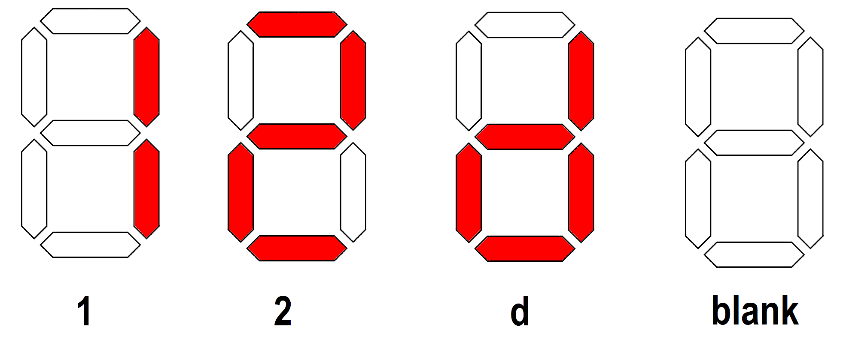
\includegraphics{ image6.png}
\caption{The illuminated patterns displayed on the win/lose 7-segment display.}
\label{fig:winLose7seg}
\end{figure}

You will use a case statement, based on the information in Table~\ref{table:winLooseTt}, to
realize this function. In the sevenSeg column put the 7-bit code needed
to illuminate the winLose 7-segment display to indicate the outcome of
the game. In the Note column put either ``1'', ``2'', ``Draw'', or
``Blank'' depending on the outcome of the game and button press. Use the
bit order given in Figure~\ref{figure:throw7seg}.

\begin{longtable}[]{@{}
  >{\raggedright\arraybackslash}p{(\columnwidth - 8\tabcolsep) * \real{0.1723}}|
  >{\raggedright\arraybackslash}p{(\columnwidth - 8\tabcolsep) * \real{0.2093}}|
  >{\raggedright\arraybackslash}p{(\columnwidth - 8\tabcolsep) * \real{0.2055}}||
  >{\raggedright\arraybackslash}p{(\columnwidth - 8\tabcolsep) * \real{0.2188}}|
  >{\raggedright\arraybackslash}p{(\columnwidth - 8\tabcolsep) * \real{0.1941}}@{}}
\caption{\protect\hypertarget{_Ref30701411}{}{}Abbreviated
truth table for the winLose module.}\tabularnewline
\toprule()
\begin{minipage}[b]{\linewidth}\raggedright
button
\end{minipage} & \begin{minipage}[b]{\linewidth}\raggedright
p1Play
\end{minipage} & \begin{minipage}[b]{\linewidth}\raggedright
p2Play
\end{minipage} & \begin{minipage}[b]{\linewidth}\raggedright
sevenSeg
\end{minipage} & \begin{minipage}[b]{\linewidth}\raggedright
Note
\end{minipage} \\
\midrule()
\endfirsthead
\toprule()
\begin{minipage}[b]{\linewidth}\raggedright
button
\end{minipage} & \begin{minipage}[b]{\linewidth}\raggedright
p1Play
\end{minipage} & \begin{minipage}[b]{\linewidth}\raggedright
p2Play
\end{minipage} & \begin{minipage}[b]{\linewidth}\raggedright
sevenSeg
\end{minipage} & \begin{minipage}[b]{\linewidth}\raggedright
Note
\end{minipage} \\ \hline
\midrule()
\endhead
0 & & & & \\ \hline
0 & & & & \\ \hline
0 & & & & \\ \hline
0 & & & & \\ \hline
0 & & & & \\ \hline
0 & & & & \\ \hline
0 & & & & \\ \hline
0 & & & & \\ \hline
0 & 10 (scissors) & 00 (rock) & 7'b0100100 & 2 \\ \hline
0 & & & & \\ \hline
0 & & & & \\ \hline
0 & & & & \\ \hline
0 & & & & \\ \hline
0 & & & & \\ \hline
0 & & & & \\ \hline
0 & & & & \\ \hline
1 & xx (don't care) & xx (don't care) & 7'b1111111 & Blank \\
\bottomrule()
\label{table:winLooseTt}
\end{longtable}

\protect\hypertarget{winLoose_Verilog}{}{}Incorporate the following into
your winLose Verilog module: Use the module and port names given in
Figure~\ref{fig:sysArch}.

\begin{itemize}
\item
  Use the module declaration:
\verb+ module winLose(p1Play, p2Play, playButton, sevenSeg);+

\item
  Use vectors for the p1Play and p2Play inputs.
\item
  Use a vector for the sevenSeg output.
\item
  Make the input port types ``wire''. Make the output port types  ``reg''.

\item
  You will use a case statement, embedded in an always statement to
  realize this module.

  \begin{itemize}
  \item
    Use brackets to make the vector for the case statement. For example,
    if button was a 1-bit signal and play was a 2-bit signal, then
    
\begin{lstlisting}[language=Verilog, frame=single]
case ({button, play})
    3'b000:  seg = 7'b1000000;    // display ``0''
    3'b001:  seg = 7'b1111001;    // display ``1''
    3'b010:   seg = 7'b0100100;    // display ``2''
    3'b011:   seg = 7'b0110000;    // display ``3''
    default:  seg = 7'b1111111;    // blank 7-seg
endcase
    \end{lstlisting}
    
  \end{itemize}

This code snippet will use the 3-bit value (button as MSB and play as
least significant 2-bits) to select one of the rows. Note that the
default case handles all the combinations where button is 1.

\item
  Use a default case (last in the list) to handle all the situations
  where the button is not pressed. The default case catches any
  unspecified input combinations for the case statement. List the
  default as the last row in the case list.
\item
  At the end of each ``case'' row, provide a comment that lists player
  1's throw, player 2's throw and the output that is displayed on the
  7-segment display. For example, in my program the first case row has a
  comment that looks like:

\verb+ // P1: Rock P2:Rock Draw +

\item
  Use the hex2Seven module from lab 2 as the starting point for this
  module.
\end{itemize}

\hypertarget{rpsgame-module}{%
\section{Module: rpsGame}
\label{rpsgame-module}}

The rpsGame module, ``glues'' together the modules shown in Figure~\ref{fig:sysArch} and
serves as the top-level entity. The Verilog code for this module
consists of 5 instantiation statements; one of them is given as the last
bullet point item in the list below. For this module, I want you to:

\begin{itemize}
\item
  Use the module declaration: \newline
   \verb+ module rpsGame(p1Throw, p1SevenSeg, p2Throw, p2SevenSeg, playButton, winLoseSeg);+

\item
  Make the p1Throw and p2Throw inputs vectors with the MSB coming from
  the rock slide-switch input and scissors slide-switch as the LSB. You
  will need to keep this consistent with the pin assignment that you
  will complete next.
\item
  The \verb+playButton+ input is not a vector.
\item
  Use a vector for the \verb+winLoseSeg+ output.
\item
  Make the input and output port types ``wire''.
\item
  You need to create 2 internal vectors. Look carefully at Figure~\ref{fig:sysArch} and
  find wires that begin and end inside the rpsGame module. These are the
  vectors.
\item
  Name the module instances using the names provided in Figure~\ref{fig:sysArch}.
\item
  When you instantiate a module

  \begin{itemize}
  \item
    The first term is the name of the module you are instantiating
  \item
    The second term is the instance name of the module
  \item
    The remaining term is the parenthesis list of signal in and out of
    the module. The order of the signals in the instantiation must be
    the same as those in the module declaration. \uline{Pay special
    attention to this!}
  \item
    For example, in my program I had an instantiation that looked like: \\
   \verb+onesToDense p1o2d(p1Throw, p1Dense);+
  \end{itemize}
\end{itemize}


\hypertarget{pin-assignment}{%
\section{Pin Assignment:}\label{pin-assignment}}

Use the image of the Development Board in Figure~\ref{figure:systemIO} and the information
in the board User Guide to determine the FPGA pins associated with the
input and output devices used by the rpsGame module.

\begin{longtable}[]{@{}
  >{\raggedright\arraybackslash}p{(\columnwidth - 6\tabcolsep) * \real{0.2500}}|
  >{\raggedright\arraybackslash}p{(\columnwidth - 6\tabcolsep) * \real{0.2500}}|
  >{\raggedright\arraybackslash}p{(\columnwidth - 6\tabcolsep) * \real{0.2500}}|
  >{\raggedright\arraybackslash}p{(\columnwidth - 6\tabcolsep) * \real{0.2500}}@{}}
\caption{\protect\hypertarget{rpsGame_PinAssignment}{}{}Pin
assignment tables for the Rock Paper Scissor Game.}\tabularnewline
\toprule()
\begin{minipage}[b]{\linewidth}\raggedright
Segment
\end{minipage} & \begin{minipage}[b]{\linewidth}\raggedright
Player 1 Throw
\end{minipage} & \begin{minipage}[b]{\linewidth}\raggedright
Player 2 Throw
\end{minipage} & \begin{minipage}[b]{\linewidth}\raggedright
Win/Lose
\end{minipage} \\ \hline
\midrule()
\endfirsthead
\toprule()
\begin{minipage}[b]{\linewidth}\raggedright
Segment
\end{minipage} & \begin{minipage}[b]{\linewidth}\raggedright
Player 1 Throw
\end{minipage} & \begin{minipage}[b]{\linewidth}\raggedright
Player 2 Throw
\end{minipage} & \begin{minipage}[b]{\linewidth}\raggedright
Win/Lose
\end{minipage} \\ \hline
\midrule()
\endhead
seg{[}6{]} & PIN\_Y18 & & \\ \hline
seg{[}5{]} & & PIN\_AC23 & \\ \hline
seg{[}4{]} & & & \\ \hline
seg{[}3{]} & & & \\ \hline
seg{[}2{]} & & & \\ \hline
seg{[}1{]} & & & \\ \hline
seg{[}0{]} & & & PIN\_AA18 \\
\bottomrule()
\end{longtable}

\begin{longtable}[]{@{}
  >{\raggedright\arraybackslash}p{(\columnwidth - 4\tabcolsep) * \real{0.3333}}|
  >{\raggedright\arraybackslash}p{(\columnwidth - 4\tabcolsep) * \real{0.3334}}|
  >{\raggedright\arraybackslash}p{(\columnwidth - 4\tabcolsep) * \real{0.3334}}@{}}
\toprule()
\begin{minipage}[b]{\linewidth}\raggedright
\end{minipage} & \begin{minipage}[b]{\linewidth}\raggedright
Player 1 Slide Switch
\end{minipage} & \begin{minipage}[b]{\linewidth}\raggedright
Player 2 Slide Switch
\end{minipage} \\ \hline
\midrule()
\endhead
slide{[}2{]} & & \\ \hline
slide{[}1{]} & & \\ \hline
slide{[}0{]} & PIN\_AC9 & \\
\bottomrule()
\end{longtable}

\begin{longtable}[]{@{}
  >{\raggedright\arraybackslash}p{(\columnwidth - 4\tabcolsep) * \real{0.3333}}|
  >{\raggedright\arraybackslash}p{(\columnwidth - 4\tabcolsep) * \real{0.3333}}|
  >{\raggedright\arraybackslash}p{(\columnwidth - 4\tabcolsep) * \real{0.3333}}@{}}
\toprule()
\begin{minipage}[b]{\linewidth}\raggedright
Play Button
\end{minipage} & \begin{minipage}[b]{\linewidth}\raggedright
Key{[}0{]}
\end{minipage} & \begin{minipage}[b]{\linewidth}\raggedright
\end{minipage} \\
\midrule()
\endhead
%\bottomrule()
\end{longtable}

Note, each push-button provides a high logic level when it is not
pressed, and provides a low logic level when pressed.

\hypertarget{turn-in}{%
\section{Turn in:}
\label{hex2seven_turn-in}}

You may work in tem of at most two. Make a record of your response to
the items below and turn them in a single copy as your team's solution
on Canvas using the instructions posted there. Include the names of both
team members at the top of your solutions. Use complete English
sentences to introduce what each of the following listed items (below)
is and how it was derived. In addition to this submission, you will be
expected to demonstrate your circuit at the beginning of your lab
section next week.

\textbf{onesToDense Module:}
\begin{itemize}
\item \protect\hyperlink{_Ref30701520}{link} Complete Table~ref{table:onesToDense} truth table for oneToDense module
\item \protect\hyperlink{ones2Dense_CanonicalSOP}{link} Canonical SOP expressions for the play{[}1{]} and play{[}0{]} functions
\item \protect\hyperlink{ones2Dense_Verilog}{link} Verilog code for the entire
module (courier 8-point font single spaced), leave out header comments.
\end{itemize}

\textbf{playToSeven Module:}
\begin{itemize}
\item \protect\hyperlink{_Ref30701476}{link} Complete Table~\ref{table:throwSevenSeg}
\item  \protect\hyperlink{play2Seven_Verilog}{link} Verilog code for the module
(courier 8-point font single spaced), leave out header comments.
\end{itemize}

\textbf{winLose Module:}
\begin{itemize}
\item \protect\hyperlink{_Ref30701411}{link} Complete Table~\ref{table:winLooseTt} truth table for winLose module
\item \protect\hyperlink{winLoose_Verilog}{link} Verilog code for the module
(courier 8-point font single spaced), leave out header comments.
\end{itemize}

\textbf{rpsGame Module:}
\begin{itemize}
\item \protect\hyperlink{play2Seven_Verilog}{link} Verilog code for the module
(courier 8-point font single spaced), leave out header comments.
\end{itemize}

\textbf{Pin Assignment:}
\begin{itemize}
\item \protect\hyperlink{rpsGame_PinAssignment}{link} Completed pin assignment
table for 7-segment, slide switches and button.
\end{itemize}


\chapter{High Low Guessing Game}
\label{chapter:RPS}
\graphicspath{ {./Lab04HighLow/Fig} }



\section{Outcomes and Objectives}

The outcome of this lab is to instantiate a guessing game using 
common logic building blocks.
on the FPGA development board. 
Through this process you will achieve the following
learning objectives.
\begin{itemize}
	\itemsep=0em
	\item \Paste{bok:REP_WordStatement}
	\item \Paste{bok:REP_TruthTable}
\end{itemize}

\section{The Guessing Game}

The guessing game is a two-person game where, one player is the guesser
and the other, an honest, secret keeper. The game starts with the secret
keeper generating a \emph{secret number} between {[}\textbf{0} and
\textbf{15}{]}, inclusive. Once the \emph{secret number} is decided, the
guesser makes a \emph{guess}, a number in the interval {[}\textbf{0} to
\textbf{15}{]} inclusive, and tells this to the secret keeper. The
secret keep then replies to the guesser if \emph{guess} is less than,
equal to, or greater than the \emph{secret number}. The game continues
with repeated guesser/secret keeper exchanges until the guesser
correctly identifies the \emph{secret number}.

\begin{figure}[ht]
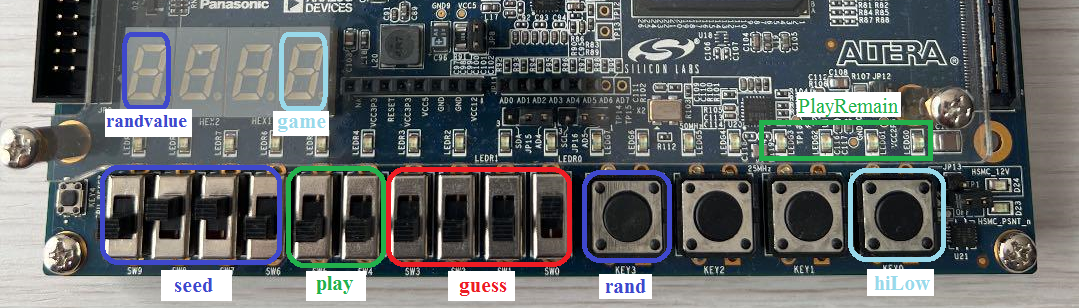
\includegraphics{image1.png}
\caption{The input and output you should use to realize the High/Low Guessing game.}
\label{fig:inputOutputDevBoard}
\end{figure}

Your goal in this lab is to create a digital version of the guessing
game using the development board using the inputs and outputs shown in
Figure~\ref{fig:inputOutputDevBoard}. In this case, the FPGA will play the role of secret keeper.
You will enter a seed value using the \textbf{seed} slide switches. The
seed value will be ``randomized'' into a 4-bit \emph{secret number}
using a linear feedback shift generator (more about this later).
Pressing the \textbf{rand} button reveals the \textbf{4}-bit
\emph{secret number} as a \textbf{1} --digit hexadecimal value on the
\textbf{randValue} 7-segment displays. Obviously, the guesser should not
press the \textbf{rand} button during regular game play.

The player will make their guess about the secret number on the
\textbf{guess} slide switches. This \emph{guess} is compared to the
\emph{secret number} and the outcome is displayed on the \textbf{game}
7-segment display when the \textbf{hiLow} button is pressed. The
\textbf{game} 7-segment display will show:

\begin{itemize}
\item   `H' when \emph{guess} \textgreater{} \emph{secret number}
\item   `I' when \emph{guess} = \emph{secret number}
\item   `L' when \emph{guess} \textless{} \emph{secret number}
\end{itemize}

A player is only allowed \textbf{4} guesses to get the secret number. To
keep track of this, every time that the player makes a guess, they
increment the binary number on the \textbf{play} slide switches. When a
slide switch is in the up position, the bit value is 1 and when in the
down position, the bit value is 0. This means that the player needs to
understand how to count in binary. In order to make keeping track of the
number of guesses remaining, the number of illuminated green
\textbf{playRemaining} LEDs will equal the number of guesses left. For
example, if the binary value set on the \textbf{play} slide switches
equals \textbf{2}, then the right-most \textbf{2} green LEDs would be
illuminated. You should illuminate LEDs starting from the right side and
increasing towards the left side.

\section{System Architecture}

There are an unlimited number of ways that you could implement this
digital system. For this lab, I want you to use the system architecture
shown in Figure~\ref{fig:guessGameSysArch}. A few comments about the visual notation used in this
schematic are in order.

\begin{enumerate}
\def\labelenumi{\arabic{enumi})}
\item
  Lines with the same name are connected together. For example, the rand
  button input is connected to the 2:1 mux in the upper left corner of
  the FPGA.
\item
  When a signal is sent to multiple devices in close proximity, a grey
  line is used to show that the signal is ``underneath a device. For
  example, the rand signal is sent to the select input of both 2:1 muxes
  in the upper left corner of the schematic. These unconnected
  connections are called ``air-wires.''
\item
  The input signals are color-coded to correspond to the colors used in
  Figure~\ref{fig:inputOutputDevBoard}.
\end{enumerate}

\begin{figure}[ht]
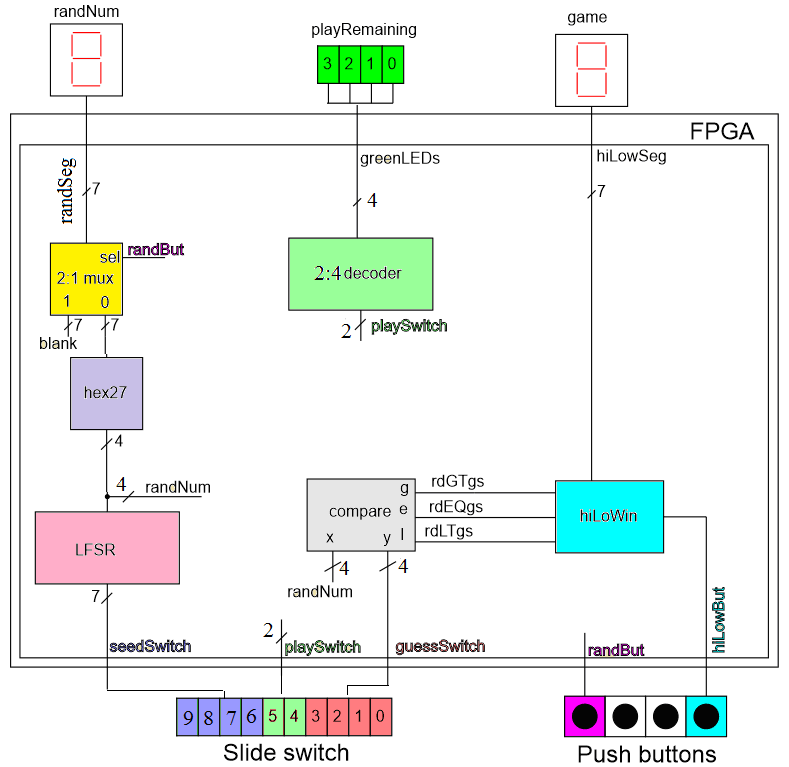
\includegraphics[width=0.6\paperwidth]{image2.png}
\caption{System architecture for the guessing game.}
\label{fig:guessGameSysArch}
\end{figure}

\section{Module: 2:1 Mux}

A 2:1 multiplexer, a mux for short, is a basic building block in many
digital systems. The 2:1 mux shown in Figure~\ref{fig:2x1MuxSymbol} routes one of the two
N-bit data inputs, \textbf{y\textsubscript{0}} or
\textbf{y\textsubscript{1}} to the N-bit output, \textbf{F}, depending
on the value of a 1-bit select signal, \textbf{s}. When \textbf{s} = 0,
\textbf{F}= \textbf{y\textsubscript{0}} and when \textbf{s} = 1,
\textbf{F}= \textbf{y\textsubscript{1}}. In other word, \textbf{F}
equals the \textbf{y} input whose subscript equals \textbf{s}.

\begin{figure}[ht]
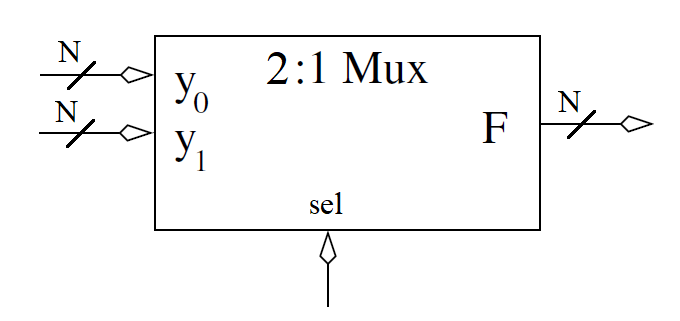
\includegraphics[width=0.4\paperwidth]{image3.png}
\caption{The schematic representation of a 2:1 mux.}
\label{fig:2x1MuxSymbol}
\end{figure}

You may notice that the data inputs of the 2:1 muxes in Figure~\ref{fig:guessGameSysArch}
 have
their \textbf{y\textsubscript{0}} and \textbf{y\textsubscript{1}} data
inputs denoted as `0' and `1' respectively. This is done to save space
and increase clarity in the schematic.

I have provided you the Verilog code for a 2:1 mux on Canvas. When
creating instances of the 2:1 mux, you will need to correctly order the
signals in the module instantiation. To do this, follow the
order shown in the module declaration shown in the top two lines in
Listing~\ref{listing:2x1muxVerilog}.

\begin{lstlisting}[language=Verilog,
 caption={Top, module definition for a 2:1 mux.  Bottom, module instantation 
 of a 2:1 mux in Figure~\ref{fig:guessGameSysArch}.},
 label={listing:2x1muxVerilog},
 frame=single]
// Module definition for the 2:1 mux
module genericMux2x1(y1, y0, sel, f);

// Module instantation for a 2:1 mux in the hiLow digital circuit
genericMux2x1 #(7) muxHex(7'b1111111, RandHex, randBut, randSeg);
\end{lstlisting}

The signal width, \textbf{N}, shown in Figure~\ref{fig:2x1MuxSymbol} is a placeholder for
some integer value in an instantiation. I designed the 2:1 mux Verilog
module so that you could specify the value of \textbf{N} using the \#()
specifier shown in the bottom line of code in Listing 1. A component
that you can instantiate with different signal widths is called
``generic''. This modifier is frequently included in the module's name.
The default value for the signal width is 8-bit. Be careful, Verilog
will allow you to instantiate a genericMux2x1 module without the \#()
specifier, defaulting to 8-bit signals for \textbf{F},
\textbf{y\textsubscript{0}} , and \textbf{y\textsubscript{0}}
\uline{and} allowing you to provide signals with different vector sizes.
It will do this with a warning that you can find in the Compilation
Report tab -\textgreater{} Analysis \& Synthesis folder -\textgreater{}
Connectivity Checks folder. Click on the offending module and you will
see the following error report. Not much, but you have been warned.

\begin{figure}[ht]
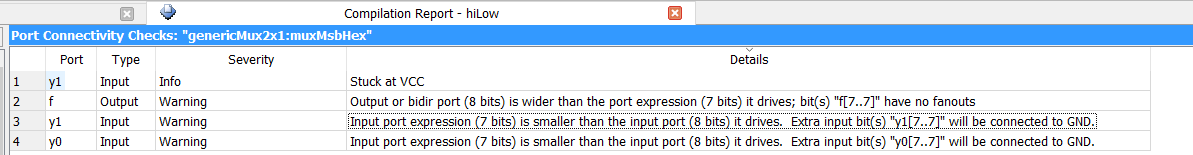
\includegraphics{image4.png}
\caption{Warning that you messed up your vector sizes in a module instantiation.}
\label{fig:vectorSizeWarnings}
\end{figure}

\hypertarget{compare-module}{%
\section{Module: Compare}\label{compare-module}}

A N-bit comparator is a basic building block in many digital systems.
The N-bit comparator shown in Figure~\ref{fig:comparatorSymbol} 
checks the relative magnitude of
the two N-bit inputs \textbf{x} and \textbf{y} and sets one of the three
outputs equal to 1, one's-hot output, depending on their relation to
each other.

\begin{figure}[ht]
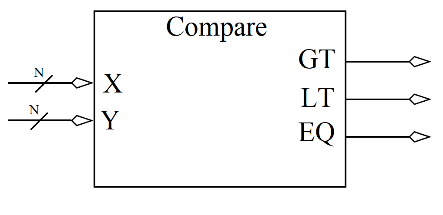
\includegraphics[width=0.4\paperwidth]{image5.png}
\caption{A schematic representation of a N-bit comparator.}
\label{fig:comparatorSymbol}
\end{figure}

The relationship between the inputs and outputs is given in the
following list. Note that the order of the inputs is important as
\textbf{X} is always on the left side of the relational operator.

\begin{itemize}
\item    \textbf{GT} = 1 when \textbf{X} \textgreater{} \textbf{Y} else  \textbf{GT} = 0
\item    \textbf{EQ} = 1 when \textbf{X} == \textbf{Y} else \textbf{EQ} = 0
\item    \textbf{LT} = 1 when \textbf{X} \textless{} \textbf{Y} else   \textbf{LT} = 0
\end{itemize}

I have provided you the Verilog code for the N-bit comparator on Canvas.
When creating instances of the comparator, you will need to correctly
order the signals in the module instantiation. To do this, follow the
order shown in the module definition shown in the top two lines in
Listing ~ref{listing:comparatorVerilog}.

\begin{lstlisting}[language=Verilog,
 caption={Top, the module definition for the comparator.  Bottom, module
 instantiation of a comparator in Figure~\ref{fig:comparatorSymbol}.},
 label={listing:comparatorVerilog},
 frame=single]
// Module definition for the comparator
module genericComparator(x, y, gt, eq, lt);

// Module instantiation for a compataror in the hiLow digital circuit
genericComparator #(4) randVsGuess(randNum, guessSwitch, \
		 randGTguess, randEQguess, randLTguess);
\end{lstlisting}

Like the mux, the comparator is a generic module. This means that you
need to specify the vector width of the \textbf{X} and \textbf{Y} inputs
using the \#() specifier. As an example, I've provided an instantiation
from my hiLow module in the lower two lines in Listing 2. Like the mux,
the default vector width for the inputs is 8-bits. Same warning about
vector size mismatch applies to comparators.


\section{Module: hexToSevenSeg}
You should use the hexToSevenSeg module you developed in a
previous lab. Note, the name of this module was shortened in Figure~\ref{fig:guessGameSysArch}
to
hex27 in order to save space and make the schematic more
readable.


\section{Module: 2:4 Decoder}


The module labeled 2:4 decoder interprets the 2-bit input
s\textsubscript{1}, s\textsubscript{0} as a 2-bit binary number that we
will call \textbf{s}. All the y outputs whose subscript is less than or
equal to \textbf{4-s} will have an output of 1. All the y outputs whose
subscript is greater than \textbf{3-s} will have an output of 0.

\begin{figure}[ht]
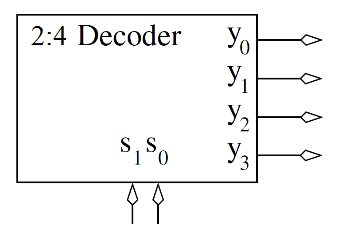
\includegraphics[width=0.3\paperwidth]{image6.png}
\caption{A 2:4 decoder.}
\label{fig:2x4decoderSymbol}
\end{figure}

The first few rows for the truth table for the 2:4 decoder are shown in
Table~\ref{table:decoderTruthTable}.

\begin{longtable}[]{@{}
 | >{\raggedright\arraybackslash}p{(\columnwidth - 10\tabcolsep) * \real{0.1688}} |
  >{\raggedright\arraybackslash}p{(\columnwidth - 10\tabcolsep) * \real{0.1688}} |
  >{\raggedright\arraybackslash}p{(\columnwidth - 10\tabcolsep) * \real{0.1696}} |
  >{\raggedright\arraybackslash}p{(\columnwidth - 10\tabcolsep) * \real{0.1696}} |
  >{\raggedright\arraybackslash}p{(\columnwidth - 10\tabcolsep) * \real{0.1617}} |
  >{\raggedright\arraybackslash}p{(\columnwidth - 10\tabcolsep) * \real{0.1617}}|@{}}
\caption{Partial truth table for the 2:4 decoder.}
\label{table:decoderTruthTable}
\tabularnewline
\toprule()
\begin{minipage}[b]{\linewidth}\raggedright
s\textsubscript{1}
\end{minipage} & \begin{minipage}[b]{\linewidth}\raggedright
s\textsubscript{0}
\end{minipage} & \begin{minipage}[b]{\linewidth}\raggedright
y\textsubscript{3}
\end{minipage} & \begin{minipage}[b]{\linewidth}\raggedright
y\textsubscript{2}
\end{minipage} & \begin{minipage}[b]{\linewidth}\raggedright
y\textsubscript{1}
\end{minipage} & \begin{minipage}[b]{\linewidth}\raggedright
y\textsubscript{0}
\end{minipage} \\
\midrule()
\endfirsthead
\toprule()
\begin{minipage}[b]{\linewidth}\raggedright
s\textsubscript{1}
\end{minipage} & \begin{minipage}[b]{\linewidth}\raggedright
s\textsubscript{0}
\end{minipage} & \begin{minipage}[b]{\linewidth}\raggedright
y\textsubscript{3}
\end{minipage} & \begin{minipage}[b]{\linewidth}\raggedright
y\textsubscript{2}
\end{minipage} & \begin{minipage}[b]{\linewidth}\raggedright
y\textsubscript{1}
\end{minipage} & \begin{minipage}[b]{\linewidth}\raggedright
y\textsubscript{0}
\end{minipage} \\
\midrule()
\endhead
0 & 0 & 1 & 1 & 1 & 1 \\ \hline
0 & 1 & 0 & 1 & 1 & 1 \\ \hline
1 & 0 & 0 & 0 & 1 & 1 \\
\bottomrule()
\end{longtable}

While this implementation may look odd, it converts the user's selection
on the \textbf{play} slide-switches to show the correct number of plays
remaining for the user on the LEDs.

You should implement the 2:4 decoder in the hiLow module using an
always/case statement similar to the one used to implement your
hexToSevenSeg. You should put this Verilog code in the hiLow module as a
(large) concurrent statement. \textbf{This means that you should not
have a separate Verilog file for the 2:4 decoder.} Remember that the
output type from an always/case statement must have the ``reg''
qualifier, not ``wire''.


\section{Module: hiLowWin}

The hiLowWin functionality converts the output from the comparator into
the illuminated patterns shown in Figure~\ref{fig:hiLowWinDisplay} 
when the \textbf{hiLow}
button is pressed. The ``I'' from ``wIn'' is needed because you cannot
make a ``W'' on a 7-segment display.

\begin{figure}[ht]
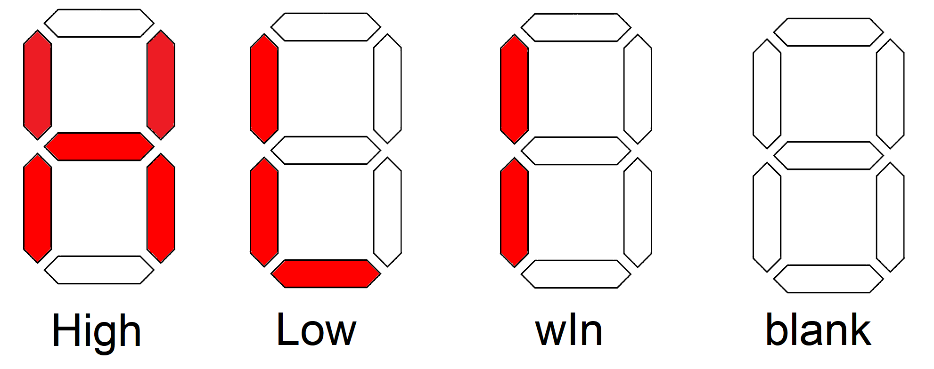
\includegraphics{image7.png}
\caption{The illuminated patterns to inform the guesser about the
magnitude of their guess.}
\label{fig:hiLowWinDisplay}
\end{figure}

You should implement hiLowWin inside the hiLow module using an
always/case statement similar to the one used to implement your
hexToSevenSeg. You will need to create a vector out of the 4-separate
inputs using the parenthesis operator as shown in Listing~\ref{listing:hiLowWinVerilog}. 
Note that the code shown Listing~\ref{listing:hiLowWinVerilog} is incomplete.

\begin{lstlisting}[language=Verilog,
 caption={Starter code for the hiLowWin module.},
 label={listing:hiLowWinVerilog},
 frame=single]
 always @(*)
	case ({hotColdBut, hotWire, warmWire, coldWire})            
		4'b0001: hotColdSeg = 7'bxxxxxxx;				
		default: hotColdSeg = 7'bxxxxxxx;
	endcase  
 \end{lstlisting}

You should put this Verilog code in the hiLow module as one of the many
concurrent statement. This means that you \uline{should not} have a
separate Verilog file for the hiLowWin. Remember that the output type
from an always/case statement must have the ``reg'' qualifier, not
``wire''.


\section{Module: LFSR}

A linear feedback shift register (LFSR) is a digital circuit that
generates a pseudo-random sequence of numbers starting from a seed
value. Since we do not yet have storage devices in our class, we will
implement a LFSR that performs a single iteration of the randomization
step as shown in Figure~\ref{fig:lfsrOperation}.

\begin{figure}[ht]
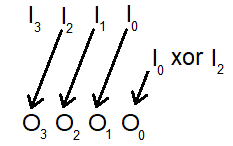
\includegraphics{image8.png}
\caption{A schematic illustration of a 4-bit LFSR operation.}
\label{fig:lfsrOperation}
\end{figure}

Figure~\ref{fig:lfsrOperation} shows 3 of the 4 input bits I\textsubscript{2} \ldots{}
I\textsubscript{0} being shifted one bit to the left on their way to the
outputs O\textsubscript{3} \ldots{} O\textsubscript{1}. The output
O\textsubscript{0} is formed by computing I\textsubscript{2} \^{}
I\textsubscript{0} where ``\^{}'' is the xor operation.

Let's use Table~\ref{table:lfsrOperations} to 
understand what happens if the input in 
Figure~\ref{fig:lfsrOperation}
was 7'b1110, which when interpreted as a decimal number is 14. The upper
3-bits of output are formed by shifting the input left by one bit. The
least significant bit of the output is formed by computing 1 \^{} 0
which equals 1. The resulting output is 7'b1101, when interpreted as a
decimal number, equals 13. Fill in the next blank row of Table 2 using
decimal 13 as an input. Repeat for the last row of the table.

\begin{longtable}[]{@{}
 | >{\raggedright\arraybackslash}p{(\columnwidth - 8\tabcolsep) * \real{0.1999}} |
  >{\raggedright\arraybackslash}p{(\columnwidth - 8\tabcolsep) * \real{0.1999}} |
  >{\raggedright\arraybackslash}p{(\columnwidth - 8\tabcolsep) * \real{0.2001}} |
  >{\raggedright\arraybackslash}p{(\columnwidth - 8\tabcolsep) * \real{0.2001}} |
  >{\raggedright\arraybackslash}p{(\columnwidth - 8\tabcolsep) * \real{0.2001}}|@{}}
\caption{The first iteration of the LFSR shown in Figure~\ref{fig:lfsrOperation} 
when started at decimal 14.}
\label{table:lfsrOperations}
\tabularnewline
\toprule()
\begin{minipage}[b]{\linewidth}\raggedright
O\textsubscript{3}
\end{minipage} & \begin{minipage}[b]{\linewidth}\raggedright
O\textsubscript{2}
\end{minipage} & \begin{minipage}[b]{\linewidth}\raggedright
O\textsubscript{1}
\end{minipage} & \begin{minipage}[b]{\linewidth}\raggedright
O\textsubscript{0}
\end{minipage} & \begin{minipage}[b]{\linewidth}\raggedright
decimal
\end{minipage} \\
\midrule()
\endfirsthead
\toprule()
\begin{minipage}[b]{\linewidth}\raggedright
O\textsubscript{3}
\end{minipage} & \begin{minipage}[b]{\linewidth}\raggedright
O\textsubscript{2}
\end{minipage} & \begin{minipage}[b]{\linewidth}\raggedright
O\textsubscript{1}
\end{minipage} & \begin{minipage}[b]{\linewidth}\raggedright
O\textsubscript{0}
\end{minipage} & \begin{minipage}[b]{\linewidth}\raggedright
decimal
\end{minipage} \\
\midrule()
\endhead
1 & 1 & 1 & 0 & 14 \\ \hline
1 & 1 & 0 & 1 & 13 \\ \hline
& & & & \\ \hline
& & & & \\
\bottomrule()
\end{longtable}

If you continued the output from the shift operation performed in Table~\ref{table:lfsrOperations} 
you would eventually find a decimal number that repeats because there
are only 16 different combinations of 4-bits. Call this repeat number
the nexus. The length of the sequence of numbers a nexus back to itself
is the length of the sequence. The length of the sequence generated by
the operation in Figure~\ref{fig:lfsrOperation} is 15. This means that if Table 2 had 15 rows
and you filled them all in, you would get 14 on the
14\textsuperscript{th} row. Can you figure out what number is excluded
from the sequence?

For the lfsr module, I want you to:

\begin{itemize}
\item
  Use the module declaration:\\
\verb+ module lfsr(Seed, outputRand);+

\item
  Make the input and outputs vectors with wire type.
\item
  \protect\hypertarget{lfsr_verilog}{}{}Use 4 assign statements to give
  each bit of output a value.
\item
  \protect\hypertarget{lfsr_testbench}{}{}Complete the testbench for the
  lfsr module. Create timing diagram that asserts the four inputs listed
  in Table~\ref{table:lfsrOperations} 
  waiting \#20 between inputs. Zoom to fill the available
  horizontal space with the waveform. Color inputs green and outputs
  red. Switch radix to unsigned decimal for input and output (right
  click on signal name in wave pane and select radix -\textgreater{}
  unsigned).
\end{itemize}

\section{Module: hiLow}

The hiLow module stiches together all the modules created and provided
to you. The hiLow module declaration contains all the signals shown in
Figure~\ref{fig:guessGameSysArch}. I've provided my module declaration here so that you can more
easily relate these to the pin assignments in the pin assignment
section.

\begin{verbatim}
module hiLow(seedSwitch, playSwitch, guessSwitch, randBut, hiLowBut,
			randSeg, greenLEDs, hiLowSeg);
\end{verbatim}

To complete this module, you will need to instantiate the modules in
Figure~\ref{fig:guessGameSysArch}. To see how to do this, I've grabbed the 2:1 mux out of the
system architecture and reproduced it in Figure~\ref{fig:snippetFromSysArch}. 
Let's write the
Verilog code to instantiate this module in the hiLow module.

\begin{figure}[ht]
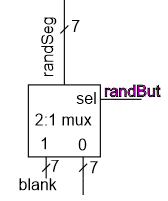
\includegraphics{image9.png}
\caption{A small piece of hardware from Figure~\ref{fig:guessGameSysArch}.}
\label{fig:snippetFromSysArch}
\end{figure}

The first step that you need to take is to give EVERY signal in the
system architecture a name or constant value. With respect to Figure~\ref{fig:snippetFromSysArch},
the output of the 2:1 mux is already named \textbf{randSeg} and the
select line is named \textbf{randBut}. The data input y1 will have a
constant value \textbf{7b'1111111}, needed to produce a blank 7-segment
display. The input y0 is the output from a hexToSevenSeg module, I named
this signal \textbf{RandHex}.

The second step is to know the order of the parameters in the 2:1 mux
module declaration. This was given earlier as:

\verb+ module genericMux2x1(y1, y0, sel, f); +


The third step is instantiating the 2:1 mux in Verilog. To do this:

\begin{itemize}
\item
  Define the width of the data input and data output of the mux
  (7-bits),
\item
  Give the 2:1 mux instance a unique name. I called my instance
  \textbf{muxHex},
\item
  Put the system architecture signals in their corresponding locations
  in the module

\verb+ genericMux2x1 #(7) muxHex(7\textquotesingle b1111111, RandHex, randBut, randSeg); +
\end{itemize}

Once you get the hang of it, you are just translating the system
architecture of Figure~\ref{fig:guessGameSysArch} into words.

For the hiLow module, I want you to:

\begin{itemize}
\item
  Use the module declaration:

\begin{verbatim}
module hiLow(seedSwitch, playSwitch, guessSwitch, randBut, hiLowBut,
		randSeg, greenLEDs, hiLowSeg); 
\end{verbatim}

\item
  Make the \verb+seedSwitch, playSwitch, seedSwitch+ inputs vectors with the
  left switch the MSB. You will need to keep this consistent with the
  pin assignment that you will compete next.
\item
  The \verb+randBut, hiLowBut+ inputs are not vectors.
\item
  Use a vector for the \verb+randSeg+ output with wire type.
\item
  Use a vector for the \verb+greenLEDs, hiLowSeg+ output with reg type.
\item
  My module had 3 internal vectors (wire type) and 3 internal one bit
  signals (shown in the system architecture).
\item
  When you instantiate a module
\item
  Run the testbench for the hiLow module provided on Canvas. Produce a
  timing diagram with the following characteristics. Zoom to fill the
  available horizontal space with the waveform. Color inputs green and
  outputs red. Order the traces from top to bottom as shown in the 
  \hypertarget{hlgg:signalColor}{following table}.

\begin{tabular}{p{4cm}p{4cm}p{4cm}}
signal & radix & color trace \\ \hline
    t\_seedSwitch & unsigned  & green  \\
    t\_guessSwitch & unsigned & green  \\
    t\_playSwitch & unsigned & green  \\
    t\_randBut & default & green  \\
    t\_hiLowBut & default & green  \\
    LFSR output & unsigned & yellow \\
    t\_randSeg & hex & red  \\
    t\_hiLowSeg & hex & red  \\
    t\_greenLEDs & default & red  \\
  \end{tabular}
\end{itemize}


\section{Pin-Assignment}

Use the image of the development board in 
Figure~\ref{fig:inputOutputDevBoard} and the information
in the board User Guide to determine the FPGA pins associated with the
input and output devices used by the hiLow module. Note, this is where I
had most of my errors.

\begin{longtable}[]{@{}
|  >{\raggedright\arraybackslash}p{(\columnwidth - 4\tabcolsep) * \real{0.3396}}|
  >{\raggedright\arraybackslash}p{(\columnwidth - 4\tabcolsep) * \real{0.3718}}|
  >{\raggedright\arraybackslash}p{(\columnwidth - 4\tabcolsep) * \real{0.2886}}|@{}}
\toprule()
\caption{Pin-Assignment for the High Low Guessing Game.}
\label{table:hlggPinAssignment} \tabularnewline
Segment & randSeg & hiLowSeg \\
\midrule()
\endhead
seg{[}6{]} & PIN\_AC22 & PIN\_Y18 \\ \hline
seg{[}5{]} & & \\ \hline
seg{[}4{]} & & \\ \hline
seg{[}3{]} & & \\ \hline
seg{[}2{]} & & \\ \hline
seg{[}1{]} & & \\ \hline
seg{[}0{]} & & \\
\bottomrule()
\end{longtable}

\begin{longtable}[]{@{}
|  >{\raggedright\arraybackslash}p{(\columnwidth - 6\tabcolsep) * \real{0.2596}} |
  >{\raggedright\arraybackslash}p{(\columnwidth - 6\tabcolsep) * \real{0.2505}} |
  >{\raggedright\arraybackslash}p{(\columnwidth - 6\tabcolsep) * \real{0.2542}} |
  >{\raggedright\arraybackslash}p{(\columnwidth - 6\tabcolsep) * \real{0.2357}}|@{}}
\toprule()
 & seedSwitch & playSwitch & guessSwitch \\ 
\midrule()
\endhead
slide{[}3{]} & PIN\_AE19 & N/A & \\  \hline
slide{[}2{]} & & N/A & \\ \hline
slide{[}1{]} & & & \\ \hline
slide{[}0{]} & & & \\
\bottomrule()
\end{longtable}

\begin{longtable}[]{@{}
|  >{\raggedright\arraybackslash}p{(\columnwidth - 4\tabcolsep) * \real{0.3334}} |
  >{\raggedright\arraybackslash}p{(\columnwidth - 4\tabcolsep) * \real{0.3334}} |
  >{\raggedright\arraybackslash}p{(\columnwidth - 4\tabcolsep) * \real{0.3333}}|@{}}
\toprule()

randBut & Key{[}3{]} & \\
\midrule()
\endhead
\begin{minipage}[t]{\linewidth}\raggedright
hiLowBut
\end{minipage} & Key{[}0{]} & \\
\bottomrule()
\end{longtable}

\begin{longtable}[]{@{}
|  >{\raggedright\arraybackslash}p{(\columnwidth - 6\tabcolsep) * \real{0.2499}} |
  >{\raggedright\arraybackslash}p{(\columnwidth - 6\tabcolsep) * \real{0.2499}} |
  >{\raggedright\arraybackslash}p{(\columnwidth - 6\tabcolsep) * \real{0.2501}} |
  >{\raggedright\arraybackslash}p{(\columnwidth - 6\tabcolsep) * \real{0.2501}}|@{}}
\toprule()
\begin{minipage}[b]{\linewidth}\raggedright
G{[}3{]}
\end{minipage} & \begin{minipage}[b]{\linewidth}\raggedright
G{[}2{]}
\end{minipage} & \begin{minipage}[b]{\linewidth}\raggedright
G{[}1{]}
\end{minipage} & \begin{minipage}[b]{\linewidth}\raggedright
G{[}0{]}
\end{minipage} \\
\midrule()
\endhead
& & & \\
\bottomrule()
\end{longtable}


\section{Turn in}

You may work in teams of at most two. Make a record of your response to
the items below and turn them in a single copy as your team's solution
on Canvas using the instructions posted there. Include the names of both
team members at the top of your solutions. Use complete English
sentences to introduce what each of the following listed items (below)
is and how it was derived. In addition to this submission, you will be
expected to demonstrate your circuit at the beginning of your lab
section next week.

\subsubsection{Module: LFSR }
\begin{itemize}
\item
  \protect\hyperlink{lfsr_verilog}{Link} Verilog code for the body of
  the module (courier 8-point font single spaced), leave out header
  comments.
\item A completed Table~\ref{table:lfsrOperations}.
\item
  \protect\hyperlink{lfsr_testbench}{Link} Complete the testbench for
  the lfsr module. Create timing diagram that asserts the four inputs
  listed in Table~\ref{table:lfsrOperations} waiting \#20 between inputs. Zoom to fill the
  available horizontal space with the waveform. Color inputs green and
  outputs red. Switch radix to unsigned decimal for input and output
  (right click on signal name in wave pane and select radix
  -\textgreater{} unsigned).
\end{itemize}

\subsubsection{Module: hiLow}


\begin{itemize}
\item
  Verilog code for the body of the hiLow module (courier 8-point
  font single spaced), leave out header comments.
\item
  Run the testbench for the hiLow module provided on Canvas.
  Produce a timing diagram according to
  \hyperlink{hlgg:signalColor}{this table}. Zoom to
  fill the available horizontal space with the waveform. 
\end{itemize}

\subsubsection{Pin-Assignment}

\begin{itemize}
\item Completed pin assignment table for all the signals in the hiLow module in Table~\ref{table:hlggPinAssignment}.
\end{itemize}


\section{Debugging Tips}
This laboratory typically generates a variety of new errors that you 
have not seen before.  As a result, I have added this section on 
useful debugging techniques to help you more effectively 
interpert the compilers output to locate errors in your code.
The following is an example story of someone debugging their code...

After I put together all the components, I ran Start Analysis \&
Elaboration. It took me a while to find and fix all my errors. I found
that by clicking on the Error icon (red x) or Warning icon (yellow
triangle) in the console area, I could eliminate a lot of the clutter
and focus on the reporting.

I defined output wire {[}7:0{]} greenLEDs; I should have used output reg
{[}7:0{]} greenLEDs; because greenLEDs is the output of an always/case
statement.

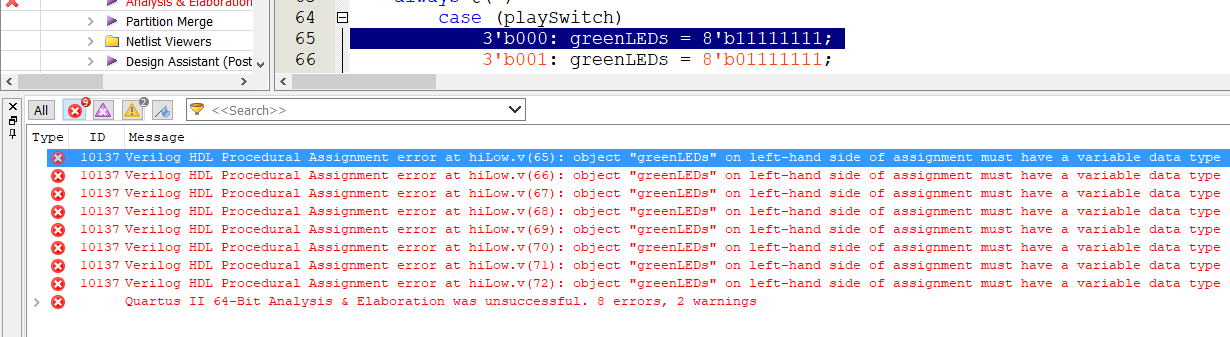
\includegraphics{image10.png}

I forgot to include the declaration of randNum -- actually I just
commented it out to get this error. The top warning always appears and
the second is a result of an unused output on my adder (more about this
in the next lab).

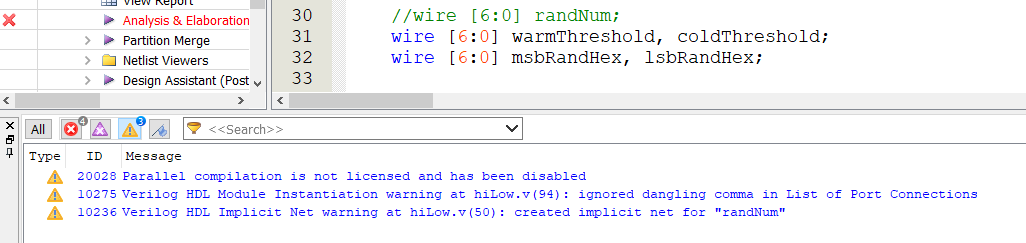
\includegraphics{image11.png}

I accidentally left a testbench as the top-level entity and tried to
synthesize.

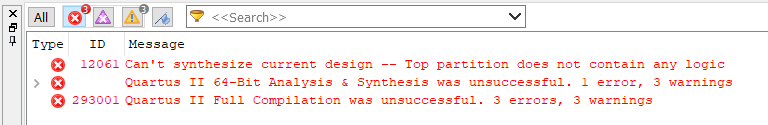
\includegraphics{image12.png}

These are all the Critical Warnings and Warnings that I got on my final,
working version. You should NOT attempt to fix these ``errors''.

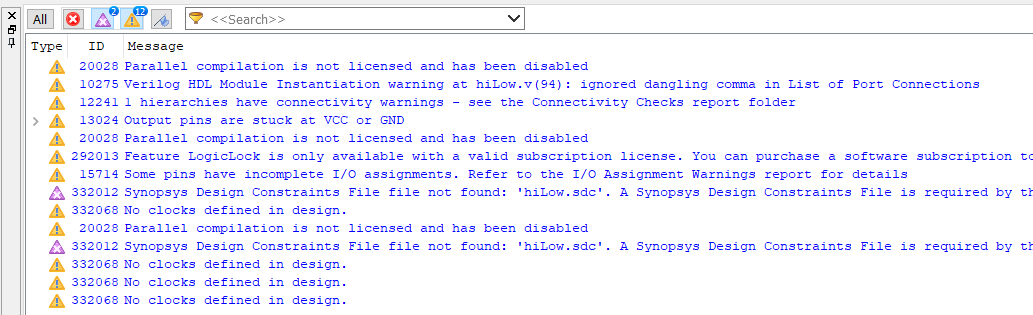
\includegraphics{image13.png}

The Connectivity Checks folder from the Compilation Report will help you
find weird connection problems that you may have inadvertently created
in your design. This report means that I hardwired one of the inputs to
the 2:1 mux to all 1's in order to blank out the 7-segment display until
the button was pressed.

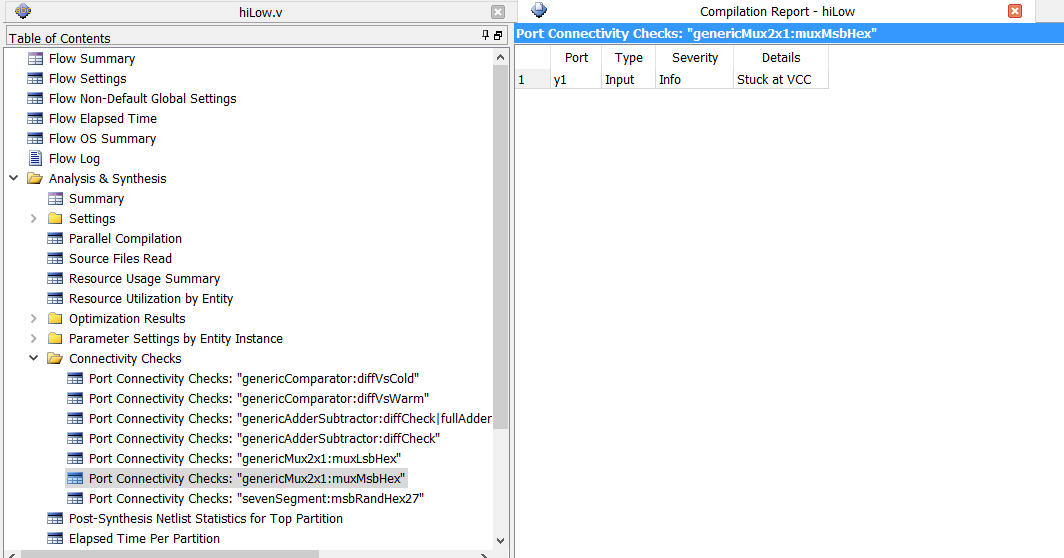
\includegraphics{image14.png}

\chapter{High Low Guessing Game With Hints}
\label{chapter:hlggwh}
\graphicspath{ {./Lab05HighLowWithHints/Fig} }



\section{Outcomes and Objectives}

The outcome of this lab is to modify existing code to add increased
functionality and instantiate it on oue development board.
Through this process you will achieve the following
learning objectives.
\begin{itemize}
	\itemsep=0em
	\item \Paste{bok:REP_WordStatement}
	\item \Paste{bok:REP_TruthTable}
\end{itemize}


\section{The Guessing Game with Hints}

This week's assignment asks you to add some enhanced functionality to
the guessing game. Since we are adding functionality to the guessing
game, it's worth reviewing the guessing game because we will use some of
the terms in the description of our enhanced functionality. The game
starts with the secret keeper generating a \emph{secret number} between
{[}0 and 15{]}, inclusive. Once the \emph{secret number} is decided, the
guesser makes a \emph{guess}, a number in the interval {[}0 to 15{]}
inclusive, and tells this to the secret keeper. The secret keep then
replies to the guesser if \emph{guess} is less than, equal to, or
greater than the \emph{secret number}. The game continues with repeated
guesser/secret keeper exchange until the guesser correctly identifies
the \emph{secret number}.

In this week's assignment, you will add circuitry to provide an
indication of how far the user's guess is from the secret number by
telling them if their \emph{guess} is hot (close to the \emph{secret
number}), warm (kind-of close to the \emph{secret number}), or cold (far
away from the \emph{secret number}).

The user input and output, shown in Figure~\ref{fig:iOonDevBorad} are the same as last week's
assignment with the exception of the \textbf{hotCold} button and
\textbf{clue} 7-segment display.

\begin{figure}[ht]
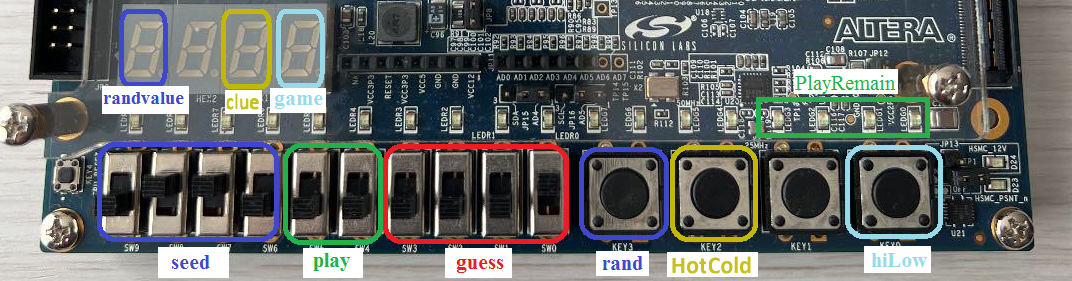
\includegraphics[width=0.8\paperwidth]{ image1.png}
\caption{The input and output you should use to realize your digital system.}
\label{fig:iOonDevBorad}
\end{figure}

The functionality of the inputs and outputs from last week's assignment
are unchanged; the \textbf{hotCold} button and \textbf{clue} 7-segment
display operate as follows.

The player can request a more refined evaluation of their guess by
pressing the \textbf{hotCold} button. To make this evaluation, the
absolute value of the difference between the \emph{guess} and
\emph{secret number} is computed and then comapred against warmThreshold
and coldThreshold as shown in Figure~\ref{fig:guessThreshold}.

\begin{itemize}
\item
  If difference \textless{} warmThreshold the guess is Hot
\item
  If (difference \textgreater= warmThreshold) and (difference
  \textless{} coldThreshold) the guess is Warm
\item
  If difference \textgreater= coldThreshold the guess is Cold
\end{itemize}

\begin{figure}[ht]
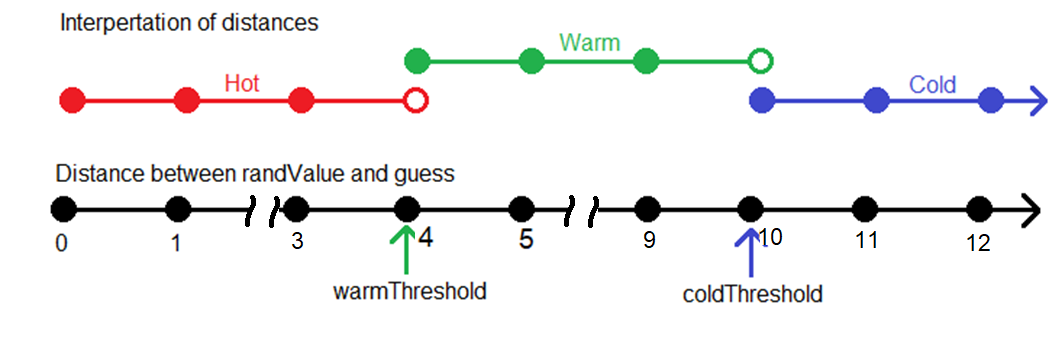
\includegraphics{ image2.png}
\caption{The interpretation of the quality of a guess in terms of thresholds.}
\label{fig:guessThreshold}
\end{figure}

The difference is always a positive number. For example, if the user's
\emph{guess} was 43 and the secret number was 45, then the difference
would be 2 making this guess Hot (according to Figure~\ref{fig:guessThreshold}). If
\emph{guess} was 45 and the \emph{secret number} was 43, the difference
would be 2 and this guess would also be Hot. Explore the relationship
between guess, secret number and the Quality of the guess by completing
Table~\ref{table:applyGuessIntervals}.

\begin{longtable}[]{@{}
|  >{\raggedright\arraybackslash}p{(\columnwidth - 6\tabcolsep) * \real{0.2499}}|
  >{\raggedright\arraybackslash}p{(\columnwidth - 6\tabcolsep) * \real{0.2499}}|
  >{\raggedright\arraybackslash}p{(\columnwidth - 6\tabcolsep) * \real{0.2501}}|
  >{\raggedright\arraybackslash}p{(\columnwidth - 6\tabcolsep) * \real{0.2501}}|@{}}
\caption{Determine the quality of a guess at the secret number.
Your answer may be a number, pair of numbers, a range or a pair of
ranges. Assume a 4-bit word size for guess and the secret number and
warmThreshold = 4 and ColdThreshold=10.}
\label{table:applyGuessIntervals}
\tabularnewline
\toprule()
\begin{minipage}[b]{\linewidth}\raggedright
\emph{guess}
\end{minipage} & \begin{minipage}[b]{\linewidth}\raggedright
\emph{secret number}
\end{minipage} & \begin{minipage}[b]{\linewidth}\raggedright
difference
\end{minipage} & \begin{minipage}[b]{\linewidth}\raggedright
Quality
\end{minipage} \\
\midrule()
\endfirsthead
\toprule()
\begin{minipage}[b]{\linewidth}\raggedright
\emph{guess}
\end{minipage} & \begin{minipage}[b]{\linewidth}\raggedright
\emph{secret number}
\end{minipage} & \begin{minipage}[b]{\linewidth}\raggedright
difference
\end{minipage} & \begin{minipage}[b]{\linewidth}\raggedright
Quality
\end{minipage} \\ 
\midrule()
\endhead
14 & 11 & & \\ \hline
8 & 12 & & \\ \hline
4 & 14 & & \\ \hline
8 & & 2 & Hot \\ \hline
& 8 & {[}4 to 9{]} & Warm \\ \hline
& 2 & {[}10 to 15{]} & Cold \\
\bottomrule()
\end{longtable}

The 7-segment display called clue will communicate the quality of the
user's guess to the user. It will do this by displaying `C' if the guess
is \textbf{\uline{C}}old, `A' if the guess is w\textbf{\uline{A}}rm, `H'
if the guess is \textbf{\uline{H}}ot.

\section{System Architecture}

There are an almost unlimited number of ways that you could implement
this digital system. For this lab, I want you to use the system
architecture shown in Figure~\ref{fig:guessWithHintSystemArch}. A few 
comments about the visual notation
used in this schematic are in order.

\begin{enumerate}
\def\labelenumi{\arabic{enumi})}
\item
  Lines with the same name are connected together.
\item
  When a signal is sent to multiple devices in close proximity, a grey
  line is used to show that the signal is ``underneath a device.
\item
  The input signals are color-coded to correspond to the colors used in
  Figure~\ref{fig:iOonDevBorad}.
\end{enumerate}

\begin{figure}[ht]
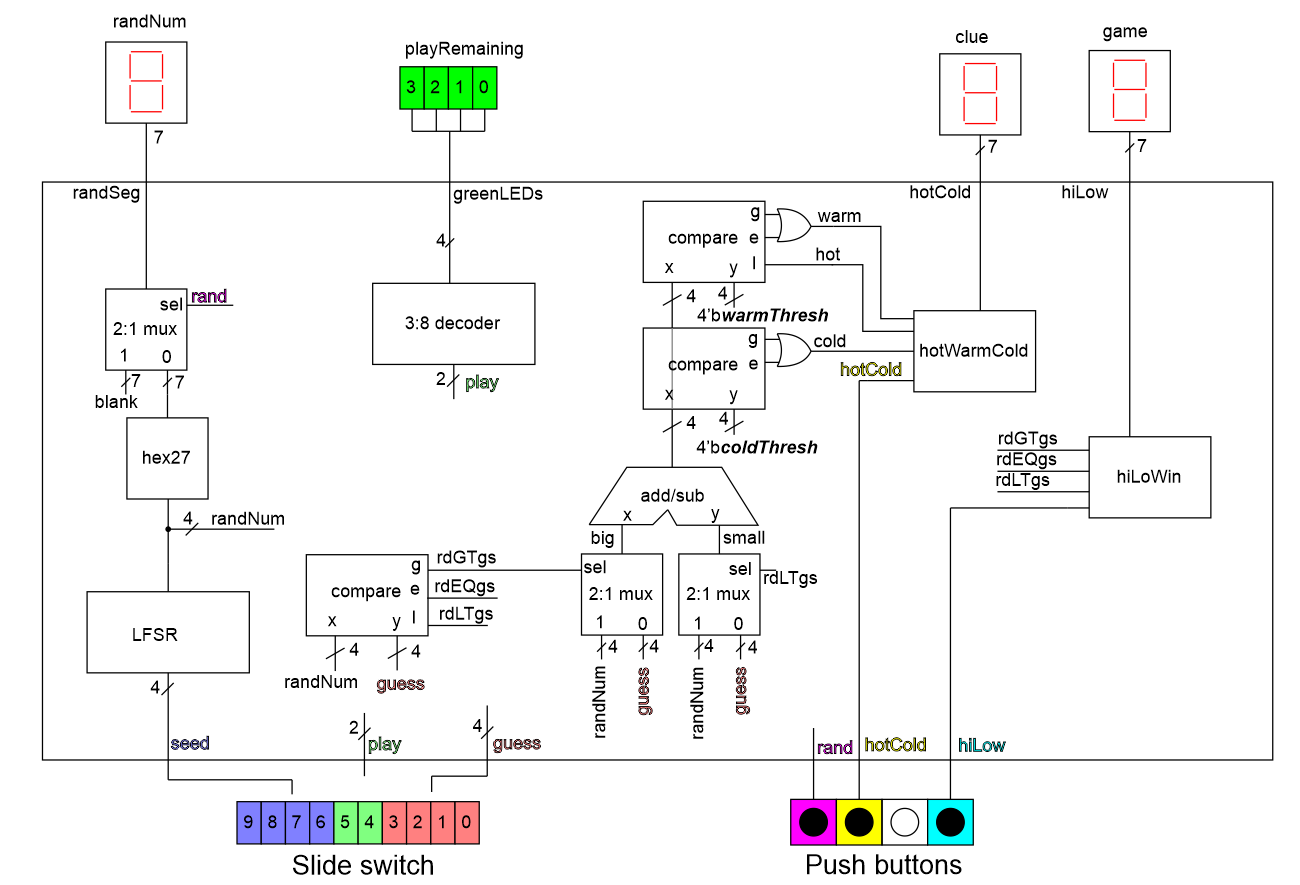
\includegraphics[width=6.50278in,height=4.42708in]{ image3.png}
\caption{System architecture for the guessing game with hint. The select
inputs on the big and small 2x1 muxes is intentionally not shown -- you
will need to figure this out.}
\label{fig:guessWithHintSystemArch}
\end{figure}

The new circuitry is shown in the middle of Figure~\ref{fig:guessWithHintSystemArch} starting with the
comparator whose inputs are \emph{randNum} and \emph{guess}. Actually,
this comparator should already be in your circuit because it provides
its outputs as the input to the hiLoWin module used in the previous lab.
This comparator is needed to determine the difference between
\emph{randNum} and \emph{guess} as follows.

The difference between the \emph{guess} and \emph{secret number} (called
\emph{randNum} in Figure~\ref{fig:guessWithHintSystemArch})that you computed 
in Table~\ref{table:applyGuessIntervals} is 
the absolute
value of the difference between \emph{guess} and the \emph{secret
number}. We will realize this functionality by placing the larger of
\emph{guess} or \emph{randNum} on the x input of the adder subtractor
shown in Figure~\ref{fig:guessWithHintSystemArch}. The smaller of \emph{guess} or \emph{randNum} is
placed on the y input of the adder subtractor. This routing of x and y
to the adder subtractor is performed by a pair of 4-bit 2x1 muxes whose
select inputs are controlled by one of the comparator's three outputs.
The adder subtractor in Figure~\ref{fig:guessWithHintSystemArch} is configured to subtract by hardwiring
its fnc input to 1'b1. You will need to determine which single output
from the comparator feeds the select input for this pair of muxes.

Let's call the output of the adder subtractor \emph{difference}. This
\emph{difference} is compared to the warmThreshold and coldThreshold
using a pair of comparators. The values of warmThresh and coldThresh are
set in code using the signal declaration and signal assignment
statements shown in Listing~\ref{listing:guessThresholds}.

\begin{lstlisting}[language=Verilog,
 caption={The signal declaration and assignment for guess thresholds.},
 label={listing:guessThresholds},
 frame=single]
    wire [3:0] warmThreshold, coldThreshold; 
    assign warmThreshold = 4'b0100;		
    assign coldThreshold = 4'b1010;
\end{lstlisting}

The output from the warmThreshold and coldThreshold comparators is used
as input to the hotWarmCold logic to display an appropriate character on
the \textbf{hotCold} 7-segment display. You will derive this logic as
you work through this lab.

\section{Module: 2:1 Mux}
This module was discussed in Lab 4.



\section{Module: Compare}
This module was discussed in Lab 4.


\section{Module: Add/Sub }

A N-bit adder subtractor is a basic building block in many digital
systems. The N-bit adder subtractor shown in Figure~\ref{fig:adderSubSymbol} adds 
its N-bit
input x and N-bit input y when fnc = 0 and places the result on the
N-bit output subDiff. When fnc = 1 the sumDiff output equals x-y. When
the inputs and output are interpreted as a 2's complement values, the
sovf output equals 1 when the computation results in an overflow. When
the inputs and output are interpreted as binary numbers, the uovf output
equals 1 when the computation results in an overflow.

\begin{figure}[ht]
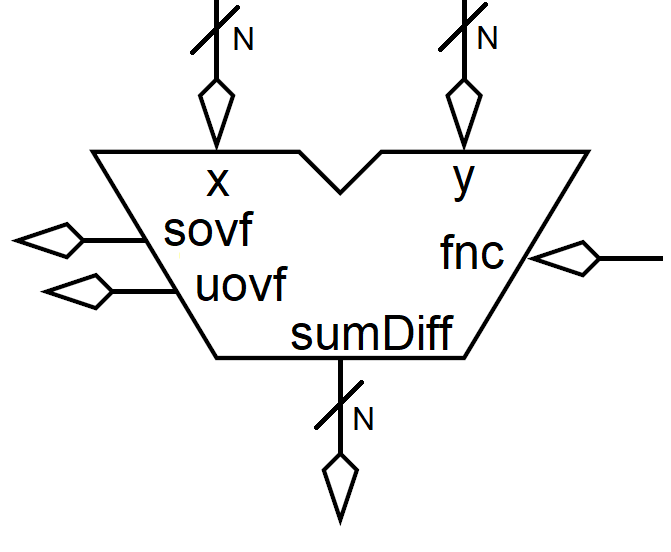
\includegraphics[width=0.3\paperwidth]{ image4.png}
\caption{A schematic representation of a N-bit adder subtractor.}
\label{fig:adderSubSymbol}
\end{figure}

I have provided you the Verilog code for the N-bit adder subtractor on
Canvas. This module instantiates N full-adders. Thus, you will need to
include the full adder module contained in the file fullAdder.v in your
project to instantiate a genericAdderSubtractor instance. Listing 2
shows the module declaration for the genericAdderSubtractor. Note that
the output from the module follows the fnc input. The module
instantiation shown in Listing 2 corresponds to the system architecture
shown in Figure~\ref{fig:guessWithHintSystemArch}. Since the inputs to the adder subtractor in the
system architecture will not generate overflow, the overflow outputs
from this adder subtractor are not needed. When you do not need an
output from a module, you can leave its parameter slot unfilled. This
explains the pair of empty fields at the end of the module instantiation
shown in Listing 2.

\begin{lstlisting}[language=Verilog,
 caption={Top, module definition for an adder subtractor.  Bottom, module instantation 
 of the adder subtractor in Figure~\ref{fig:guessWithHintSystemArch}.},
 label={listing:adderSubtractor},
 frame=single]
// Module definition for the comparator
module genericAdderSubtractor(a, b, fnc, sumDiff, sovf, uovf);

// Module instantiation for an adder subtractor in hiLow digital circuit
genericAdderSubtractor #(4) prox(big, small, 1'b1, difference, , );
\end{lstlisting}


Like the mux and comparator, the adder subtractor is a generic module.
This means that you need to specify the vector width of the \textbf{X}
and \textbf{Y} inputs and \textbf{sumDiff} output using the \#()
specifier. Pay close attention to match the value of this generic and
the size of the input and output vectors.


\section{Logic: hotWarmCold}

The goal of this section is to determine the logic inside the hotWarmCold logi blok
in Figure~\ref{fig:guessWithHintSystemArch}.  To do this you will first need to form three 
signals, \emph{hot}, \emph{warm}, and \emph{cold}.  These three signals describe how close the 
\emph{guess} is from \emph{randNum}. We will call the comparator that compares \emph{difference} 
and \emph{warmThresh}, the warm comparator and call its three outputs wGT, wEQ and wLT.
The other omprtor is the cold comparator nd its outputs preixed with  lowercase ``c''.

The warm and cold comparators generate a total of 6 signals, some of which are
sent to the logic block B1 and B2 to form the warm and cold signals - the logic for the
hot signal is given to you in Figure~\ref{fig:guessWithHintSystemArch}.

To understand the logic inside the B1 and B2 logic blocks let's look at an
example.  Use \emph{coldThresh} = 10 and \emph{warmThresh} = 4 to complete
Table~\ref{table:fillInCompareOperations}.  Do this by comparing the value in the column labeled
``\emph{difference}'' to \emph{warmThresh} and \emph{coldThresh} and
asserting the appropriate comparators outputs.  It may help for us to do one 
row together, \emph{difference} = 9. If we consider the
warm comparator, the x input equals 9 (the value of \emph{difference})
and the y input equals 4 (the value of \emph{warmThresh}). Since 9 is
greater than 4, the output wGT will equal 1 and wEQ and wLT will both
equal 0. If we consider the cold comparator, the x input equals 9 (the
value of \emph{difference}) and the y input equals 10 (the value of
\emph{coldThresh}). Since 9 is less than 10, the output cLT will equal 1
and cEQ and cGT will both equal 0. Finally, since \emph{difference}
equals 9 and this is between the warm and cold thresholds, the quality
of the guess should set warm = 1 and hot and cold to 0.

\begin{longtable}[]{@{}
| >{\raggedright\arraybackslash}p{(\columnwidth - 18\tabcolsep) * \real{0.1110}}|
  >{\raggedright\arraybackslash}p{(\columnwidth - 18\tabcolsep) * \real{0.1004}}|
  >{\raggedright\arraybackslash}p{(\columnwidth - 18\tabcolsep) * \real{0.1004}}|
  >{\raggedright\arraybackslash}p{(\columnwidth - 18\tabcolsep) * \real{0.1005}}|
  >{\raggedright\arraybackslash}p{(\columnwidth - 18\tabcolsep) * \real{0.1004}}|
  >{\raggedright\arraybackslash}p{(\columnwidth - 18\tabcolsep) * \real{0.1004}}|
  >{\raggedright\arraybackslash}p{(\columnwidth - 18\tabcolsep) * \real{0.1005}}|
  >{\raggedright\arraybackslash}p{(\columnwidth - 18\tabcolsep) * \real{0.0957}}|
  >{\raggedright\arraybackslash}p{(\columnwidth - 18\tabcolsep) * \real{0.0957}}|
  >{\raggedright\arraybackslash}p{(\columnwidth - 18\tabcolsep) * \real{0.0951}}@{}|}
\caption{Complete the following table to determine which
comparator outputs are needed to determine the quality of a guess. Let
warmThresh = 4 and coldThresh = 10.}\label{table:fillInCompareOperations}\tabularnewline
\toprule()
\multirow{2}{*}{difference} & 
	\multicolumn{3}{|c|}{warmThresh comparator} & 
	\multicolumn{3}{|c|}{coldThresh comparator} & 
	\multirow{2}{*}{Hot} &
	\multirow{2}{*}{Warm} & 
	\multirow{2}{*}{Cold} \\ \cline{2-7}
& wGT & wEQ & wLT & cGT & cEQ &  \\ \cline{2-7}
\midrule()
\endfirsthead
\toprule()
\multirow{2}{*}{difference} & 
	\multicolumn{3}{|c|}{warmThresh comparator} & 
	\multicolumn{3}{|c|}{coldThresh comparator} & 
	\multirow{2}{*}{Hot} &
	\multirow{2}{*}{Warm} & 
	\multirow{2}{*}{Cold} \\ \cline{2-7}
& wGT & wEQ & wLT & cGT & cEQ &  \\ \cline{2-7}
\midrule()
\endhead
3 & & & & & & & & & \\ \hline
4 & & & & & & & & & \\ \hline
5 & & & & & & & & & \\ \hline
9 & 1 & & & & & 1 & & 1 & \\ \hline
10 & & & & & & & & & \\ \hline
11 & & & & & & & & & \\
\bottomrule()
\end{longtable}

Now, you need to use the values in Table~\ref{table:fillInCompareOperations} to determine the logic for
each of the three outputs from the ``discrete logic'' block shown in
Figure~\ref{fig:guessWithHintSystemArch}. To do this, look at the conditions that cause each of the
outputs and write an expression using AND and OR to describe when that
output equals 1.  You 

\protect\hypertarget{hotWarmCold_Logic}{}{}
\begin{verbatim}
	Cold =                               // write logic description
	Warm =                            // write logic description
	Hot = wLT;                       // given to you in  Figure~\ref{fig:guessWithHintSystemArch}
\end{verbatim}

For the hotWarmCold block of code:

\begin{itemize}
\item
  Make three assign statements, one for hot, warm and cold
\item
  Use only \& and \textbar{} operations.
\item
  Use parenthesis to ensure proper order of operation.
\item
  The \emph{hot}, \emph{warm} and \emph{cold} signals should be ``wire''
  type.
\end{itemize}

You will implement the hotWarmCold logic using an always/case statement
that takes in as input the 3 outputs from the ``discrete Logic'' block,
\emph{hot}, \emph{warm} and \emph{cold}. These three outputs form a 1's
hot code because a guess can only be one of these three conditions at a
time. When the \textbf{hotCold} button is pressed, the output of the
hotWarmCold block forms an illuminate 7-segment representation of the
quality of the guess shown in Figure~\ref{figure:hiLoHintSevenSeg}. The 
7-segment output from the
hotWarmCold block should be blank when the \textbf{hotCold} button is
unpressed.

\begin{figure}[ht]
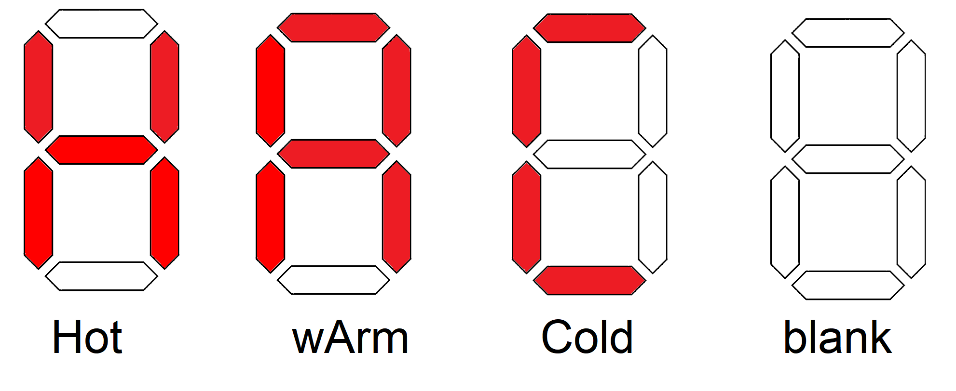
\includegraphics{ image5.png}
\caption{The illuminated patterns to inform the guesser about the magnitude of their guess.}
\label{figure:hiLoHintSevenSeg}
\end{figure}

For this block of code:

\begin{itemize}
\item
  Use an always/case statement.
\item
  Form a 4-bit vector from the \emph{hot}, \emph{warm}, \emph{cold}
  signals and the \textbf{hotCold} button.
\item
  Use this 4-bit vector as the input to the always/case statement.
\item
  Make sure that the output signal has ``reg'' type.
\item
  Include inline comments prior to the always/case statement describing
  the pattern that is displayed on the 7-segment display for each
  possible output. An example is given in Listing 3.
\end{itemize}

\begin{lstlisting}[language=Verilog,
 caption={A comment block describing the pattern of illuminated segment for each guess hint..},
 label={listing:hotColdGuess},
 frame=single]
//*********************************************
// Logic to display the quality of the guess
//	Hot  = `H' = <show binary code>
//	wArm = `A' = <show binary code>
//	Cold = `C' = <show binary code>
//
//		 hex[0]
//		 -----
//	hex[5]	|	|	hex[1]
//		|	|	
//		 -----	hex[6]
//	hex[4]	|	|
//		|	|	hex[2]
//		 -----
//		 hex[3]
//*********************************************
\end{lstlisting}


\section{Module: hiLow}
This is the top-level module in Figure~\ref{fig:guessWithHintSystemArch}, the outermost
block. \uline{If you were not able to get the previous lab working}, just
implement the functionality identified in this assignment and make the
\emph{randNum} come directly from the seed switch. In this case, you
should use the top module declaration in Listing~\ref{listing:hiLowModule}. If you got the
previous lab working correctly, then you should use the bottom
declaration in Listing~\ref{listing:hiLowModule}.



\begin{lstlisting}[language=Verilog,
 caption={The module declaration for the enhanced hiLow module if you did or did 
 not get the previous lab working.},
 label={listing:hiLowModule},
basicstyle=\tiny\ttfamily,
 frame=single]
 
 // Didn't get previous lab working, then use this module declaration
module hiLow(seedSwitch, guessSwitch, hotColdBut, hotColdSeg);

// Did you complete the previous lab successfully?  Then use this module declaration (with no line break)
module hiLow(seedSwitch, playSwitch, guessSwitch, randBut, hotColdBut, hiLowBut, randMsbSeg, randLsbSeg, 
					greenLEDs, hotColdSeg, hiLowSeg);
 \end{lstlisting}
 
The \emph{randNum} and \emph{guess} comparator is connected to the pair of 2:1 muxes 
using the rdGtgs (means random is greater than guess) signal.
 Note that \emph{randNum} and \emph{guess} are on different
inputs to the 2 muxes so that a single output of the comparator will
work for both multiplexers. Note, when \emph{randNum} and \emph{guess}
are equal, it does not matter which is routed to the x or y input
because the output of the adder subtractor will equal 0.

For this block of code:

\begin{itemize}
\item
  Instantiate genericMux2x1 using the module provided in the previous
  lab.
\item
  Instantiate genericCompare using the module provided in the previous
  lab.
\item
  Instantiate genericAddSub using the module provided in the Canvas
  folder for this lab.
\item
  Make sure to include the fullAdder module in your project.
\item
  Use descriptive names for internal signal.
\item
  Use descriptive names for component instance names.
\end{itemize}

\section{Module: hiLow\_tb}

The testbench checks hot, warm and cold for guesses that
are too high and too low. I carefully selected these values to check the
edge cases, meaning on either side of the warm and cold thresholds.
\begin{verbatim}
	warmThresh = 4'b0110 = 4
	coldThresh = 4'b0110 = 10
\end{verbatim}

Table~\ref{table:hiLowTestbenchValues} contains the values that you will use to test your circuit.
Before using the testbench, you need to understand what your circuit
should output. The signal names in the top row of Table~\ref{table:hiLowTestbenchValues} are borrowed
from the system architecture in Figure~\ref{fig:guessWithHintSystemArch}. Fill in the missing binary and
decimal values for the cells in the guess, big, small and difference
columns. In the Comment column, put the quality of the guess as either
``Hot'', ``Warm'' or ``Cold''.

\begin{longtable}[]{@{}
| >{\raggedright\arraybackslash}p{(\columnwidth - 14\tabcolsep) * \real{0.0742}}|
  >{\raggedright\arraybackslash}p{(\columnwidth - 14\tabcolsep) * \real{0.1258}}|
  >{\raggedright\arraybackslash}p{(\columnwidth - 14\tabcolsep) * \real{0.1258}}|
  >{\raggedright\arraybackslash}p{(\columnwidth - 14\tabcolsep) * \real{0.1392}}|
  >{\raggedright\arraybackslash}p{(\columnwidth - 14\tabcolsep) * \real{0.1392}}|
  >{\raggedright\arraybackslash}p{(\columnwidth - 14\tabcolsep) * \real{0.1392}}|
  >{\raggedright\arraybackslash}p{(\columnwidth - 14\tabcolsep) * \real{0.1392}}|
  >{\raggedright\arraybackslash}p{(\columnwidth - 14\tabcolsep) * \real{0.1174}}@{}|}
\caption{Table : The values used in the hiLow testbench.}\label{table:hiLowTestbenchValues}\tabularnewline
\toprule()
Test & seed & randNum & guess & big & small & Difference & Comment \\ 
\midrule()
\endfirsthead
\toprule()
Test & seed & randNum & guess & big & small & Difference & Comment \\ 
\midrule()
\endhead
1  &
	\multirow{5}{*}{4'b1010} & 
	\multirow{5}{*}{4'b0100 } &
	4'b1111 &  &
	\multirow{5}{*}{} & &  				\\ \cline{1-1}\cline{4-5}\cline{7-8}
2 & & & =14 		&  & &  & 		\\ \cline{1-1}\cline{4-5}\cline{7-8}
3 & & & 4'b1101 = 	&  & &  &  		\\ \cline{1-1}\cline{4-5}\cline{7-8}
4 & & & 4'b1000 =	& & &  &  		\\ \cline{1-1}\cline{4-5}\cline{7-8}
5 & & & 4'b0111 = 	&  & &  &  		\\ \hline

6 & 
	\multirow{6}{*}{4'b1111} &
	\multirow{6}{*}{4'b1110} & 
	4'b0011 &
	\multirow{6}{*}{} &  &  &  \\ \cline{1-1}\cline{4-4}\cline{6-8}

7  & & &  =4 & &  &  & \\ \cline{1-1}\cline{4-4}\cline{6-8}
8  & & & =5 & & &  & \\ \cline{1-1}\cline{4-4}\cline{6-8}
9  & & & 4'b1010 = & &  & &  \\ \cline{1-1}\cline{4-4}\cline{6-8}
10 & & & 4'b1011 = & & & & \\ \cline{1-1}\cline{4-4}\cline{6-8}
11 & & & 4'b1110 = & & & & \\
\bottomrule()
\end{longtable}


\section{Pin-Assignment}

Use the image of the Development Board in Figure~\ref{fig:iOonDevBorad} and the information
in the User Guide to determine the FPGA pins associated with the input
and output devices used by the hiLow module.

\begin{longtable}[]{@{}
|  >{\raggedright\arraybackslash}p{(\columnwidth - 6\tabcolsep) * \real{0.2571}}|
  >{\raggedright\arraybackslash}p{(\columnwidth - 6\tabcolsep) * \real{0.2814}}|
  >{\raggedright\arraybackslash}p{(\columnwidth - 6\tabcolsep) * \real{0.2430}}|
  >{\raggedright\arraybackslash}p{(\columnwidth - 6\tabcolsep) * \real{0.2185}}|@{}}
\toprule()
\begin{minipage}[b]{\linewidth}\raggedright
Segment
\end{minipage} & \begin{minipage}[b]{\linewidth}\raggedright
randSeg
\end{minipage} & \begin{minipage}[b]{\linewidth}\raggedright
hotColdSeg
\end{minipage} & \begin{minipage}[b]{\linewidth}\raggedright
hiLowSeg
\end{minipage} \\
\midrule()
\endhead
seg{[}6{]} & AC22 & &  \\ \hline
seg{[}5{]} &     & &  \\ \hline
seg{[}4{]} &  & &  \\ \hline
seg{[}3{]} &  & & W18 \\ \hline
seg{[}2{]} & AA23 & &  \\ \hline
seg{[}1{]} &  & &  \\ \hline
seg{[}0{]} &  & & V19 \\
\bottomrule()
\end{longtable}

\begin{longtable}[]{@{}
|  >{\raggedright\arraybackslash}p{(\columnwidth - 6\tabcolsep) * \real{0.2596}}|
  >{\raggedright\arraybackslash}p{(\columnwidth - 6\tabcolsep) * \real{0.2505}}|
  >{\raggedright\arraybackslash}p{(\columnwidth - 6\tabcolsep) * \real{0.2542}}|
  >{\raggedright\arraybackslash}p{(\columnwidth - 6\tabcolsep) * \real{0.2357}}|@{}}
\toprule()
\begin{minipage}[b]{\linewidth}\raggedright
\end{minipage} & \begin{minipage}[b]{\linewidth}\raggedright
seedSwitch
\end{minipage} & \begin{minipage}[b]{\linewidth}\raggedright
playSwitch
\end{minipage} & \begin{minipage}[b]{\linewidth}\raggedright
guessSwitch
\end{minipage} \\
\midrule()
\endhead
slide{[}3{]} & AE19 & N/A &  \\ \hline
slide{[}2{]} &  & N/A &  \\ \hline
slide{[}1{]} &  &  & AE10 \\ \hline
slide{[}0{]} &  & W11 &  \\
\bottomrule()
\end{longtable}

\begin{longtable}[]{@{}
|  >{\raggedright\arraybackslash}p{(\columnwidth - 4\tabcolsep) * \real{0.3334}}|
  >{\raggedright\arraybackslash}p{(\columnwidth - 4\tabcolsep) * \real{0.3334}}|
  >{\raggedright\arraybackslash}p{(\columnwidth - 4\tabcolsep) * \real{0.3333}}|@{}}
\toprule()
\begin{minipage}[b]{\linewidth}\raggedright
randBut
\end{minipage} & \begin{minipage}[b]{\linewidth}\raggedright
Key{[}3{]}
\end{minipage} & \begin{minipage}[b]{\linewidth}\raggedright
Y16
\end{minipage} \\
\midrule()
\endhead
\begin{minipage}[t]{\linewidth}\raggedright
hotColdBut
\end{minipage} & Key{[}2{]} & \\ \hline
\begin{minipage}[t]{\linewidth}\raggedright
hiLowBut
\end{minipage} & Key{[}0{]} &  \\
\bottomrule()
\end{longtable}

\begin{longtable}[]{@{}
| >{\raggedright\arraybackslash}p{(\columnwidth - 6\tabcolsep) * \real{0.2499}}|
  >{\raggedright\arraybackslash}p{(\columnwidth - 6\tabcolsep) * \real{0.2499}}|
  >{\raggedright\arraybackslash}p{(\columnwidth - 6\tabcolsep) * \real{0.2501}}|
  >{\raggedright\arraybackslash}p{(\columnwidth - 6\tabcolsep) * \real{0.2501}}|@{}}
\toprule()
\begin{minipage}[b]{\linewidth}\raggedright
G{[}3{]}
\end{minipage} & \begin{minipage}[b]{\linewidth}\raggedright
G{[}2{]}
\end{minipage} & \begin{minipage}[b]{\linewidth}\raggedright
G{[}1{]}
\end{minipage} & \begin{minipage}[b]{\linewidth}\raggedright
G{[}0{]}
\end{minipage} \\
\midrule()
\endhead
E9 &  &  &  \\
\bottomrule()
\end{longtable}

\section{Turn in}

You may work in teams of at most two. Make a record of your response to
the items below and turn them in a single copy as your team's solution
on Canvas using the instructions posted there. Include the names of both
team members at the top of your solutions. Use complete English
sentences to introduce what each of the following listed items (below)
is and how it was derived. In addition to this submission, you will be
expected to demonstrate your circuit at the beginning of your lab
section next week.

\subsubsection{System Architecture}
\begin{itemize}
\item Complete Table~\ref{table:applyGuessIntervals}.
\end{itemize}

\subsubsection{Discrete Logic block}
\begin{itemize}
\item Complete Table~\ref{table:fillInCompareOperations}

\item \protect\hyperlink{hotWarmCold_Logic}{Link} Logic for hot, warm, and
cold signals
\end{itemize}


\subsubsection{Module: hiLow}

\begin{itemize}
\item
  \protect\hyperlink{hilow-module}{Link} Verilog code for the body of
  the hiLow module (courier 8-point font single spaced), leave out
  header comments.
\item
  Complete Table~\ref{table:hiLowTestbenchValues}.
\item
  \protect\hyperlink{hilow_tb-module}{Link} Run the testbench for the
  hiLow module provided on Canvas. Produce a timing diagram with the
  following characteristics. Zoom to fill the available horizontal space
  with the waveform. Color inputs green and outputs red. Order the
  traces from top to bottom as

  \begin{tabular}{p{4cm}p{4cm}p{4cm}}
   signal & radix & trace color \\ \hline
    seedSwitch  &  unsigned & Green  \\
    randNum  &  unsigned  & Lime green  \\
    GuessSwitch  &  unsigned  & Lime green  \\
    Big   & unsigned &  Cyan  \\
    Small  &  unsigned &  Cyan  \\
    Difference  &  unsigned &  Blue  \\
    hotWire  & default &  Orange  \\
    warmWire  & default &  Orange  \\
    coldWire  & default &  Orange  \\
    hotColdSeg  & hexadecimal &  Red  \\
\end{tabular}

I do not want the signals from the testbench, but rather the signals
from inside the hiLow module. You can do this in ModelSim, by expanding
the hiLow\_tb instance in the left ModelSim pane shown in Figure~\ref{fig:hierarchyTestbench} and
selecting ``uut''. Since uut is an instance of the hiLow module, all the
signals accessible in the hiLow module are shown in the center Object
pane in Figure~\ref{fig:hierarchyTestbench}. You can add any of these signals by clicking on them
and dragging them into the rightmost Wave pane shown in Figure~\ref{fig:hierarchyTestbench}.

\begin{figure}[ht]
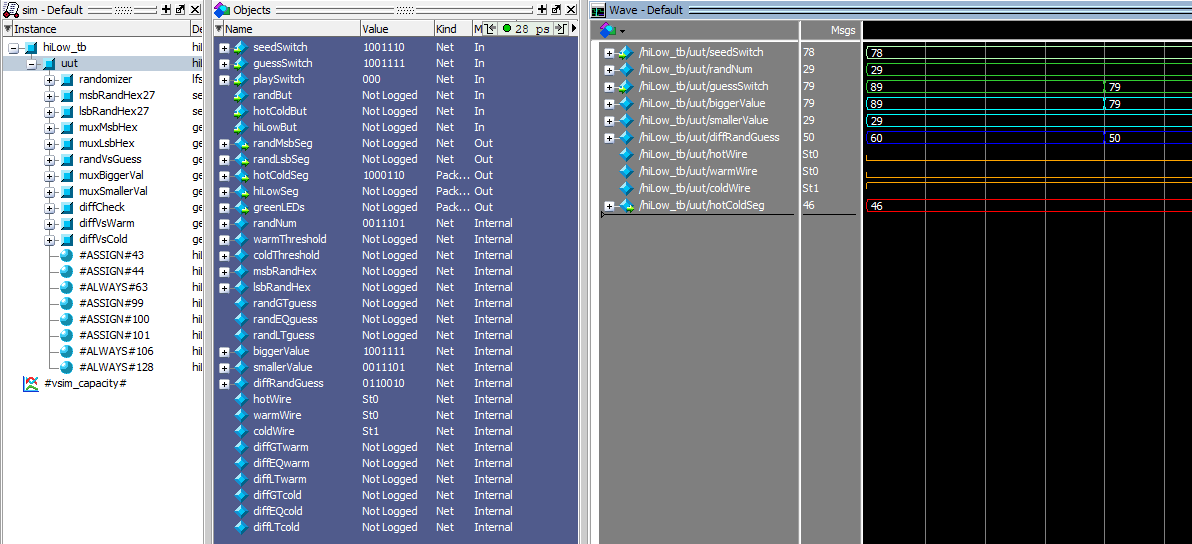
\includegraphics{ image6.png}
\caption{Use the design hierarchy to add signals to the testbench.}
\label{fig:hierarchyTestbench}
\end{figure}

When compete, your testbench should look like the timing diagram in
Figure~\ref{fig:guessTiming}.

\begin{figure}[ht]
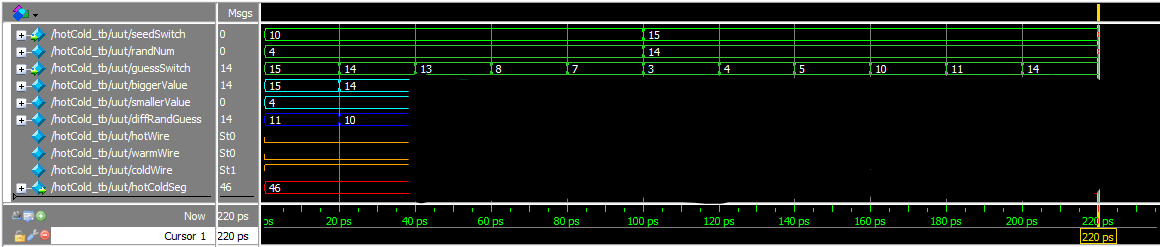
\includegraphics{ image7.png}
\caption{A partially obscured timing diagram generated by the testbench.}
\label{fig:guessTiming}
\end{figure}
\end{itemize}

\subsubsection{Demo}
\begin{itemize}
\item Demonstrate your completed circuit by the start of next week's lab.
\end{itemize}

\section{Debugging Tips}

When my program executed successfully, I got the warnings shown in
Figure~\ref{fig:messageConsole}. These are mainly the result of the unused overflow outputs
from the adder subtractor. You can filter out all the compile messages
by clicking on the yellow triangle (with the blue three in this case) on
the top line of the console window. Note, if there are several related
warnings, they will have one top-level warning with all the instances
accessible by clicking the expander arrow (it looks like
``\textgreater'') to the left of the warning triangle.

\begin{figure}[ht]
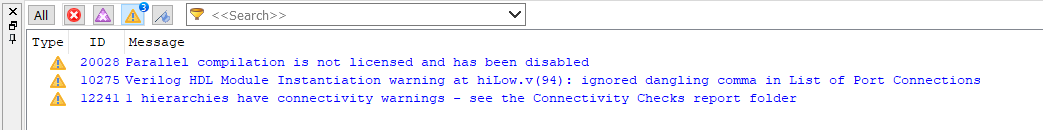
\includegraphics{image8.png}
\caption{The messages console filtered by warnings.}
\label{fig:messageConsole}
\end{figure}

I have found the Connectivity Checks folder in the Compilation Report to
help me quickly track down errors. To use it, open the Connectivity
Checks folder, click on a Port Connectivity Checks item and read the
report in the right pane. In the report shown in Figure~\ref{fig:connectivityCheck}, I selected
the genericAdderSubtractor and note I hardwired fnc to 1 so that it
always subtracts. This report also shows that the overflow outputs are
unconnected because we left them open using a pair of commas talked
about earlier.

\begin{figure}[ht]
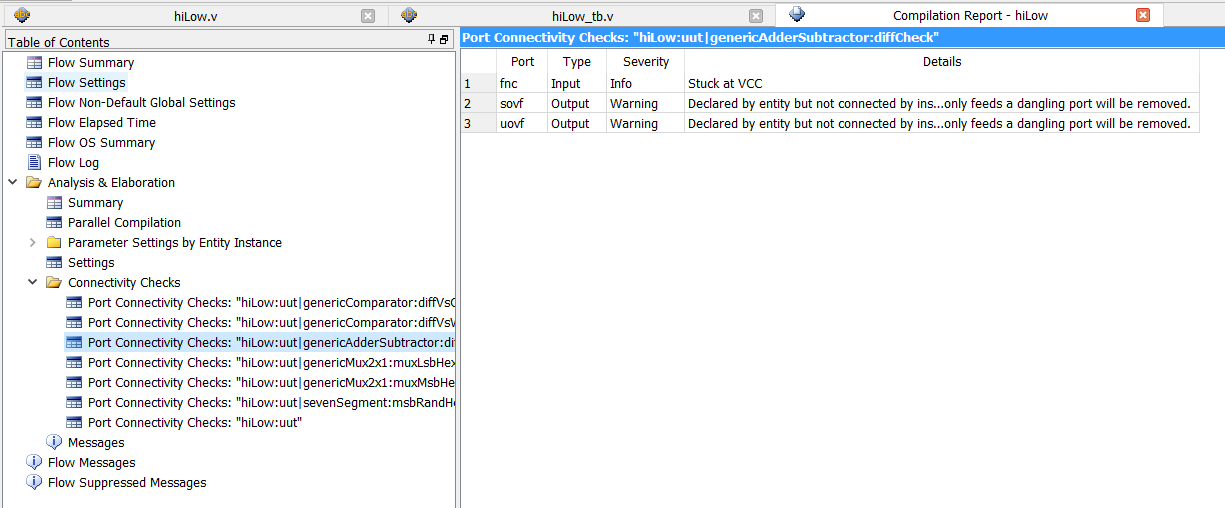
\includegraphics{ image9.png}
\caption{Connectivity Checks report for a working hiLow circuit.}
\label{fig:connectivityCheck}
\end{figure}


\chapter{Calculator With Friendly Output}
\label{chapter:calc}
\graphicspath{ {./Lab06Calculator/Fig} }

\hypertarget{objective}{%
\section{\texorpdfstring{Objective }{Objective }}\label{objective}}

The objective of this lab is to modify existing code to add increased
functionality. The design requires utilization of basic building block
and custom combinational logic blocks to realize a complex digital
circuit.

\subsubsetion{Basic Calculator}

This week you are going to build a very basic calculator that can add or
subtract 4-bit values. On the surface, this should require nothing more
than connecting some slide switches to the x and y inputs of an
adder/subtractor which sends its output to a 7-segment display. And for
the most part this is correct. However, instead of displaying the input
and output of the adder as hexadecimal values, you will display them as
2-digit decimal values. The user input and output are shown in Figure~\ref{fig:calcDevBoard}.
The user enters a pair of 4-bit operands using the left-most slide
switches, \textbf{xSlide} and \textbf{ySlide}. The value entered for
\textbf{xSlide} is displayed on the two (red) \textbf{xDisplay}
7-segment displays. The value entered for \textbf{ySlide} is displayed
on the two (green) \textbf{yDisplay} 7-segment displays. The leftmost
the \textbf{addSub} buttons specify the operation performed on
\textbf{xSlide} and \textbf{ySlide}. The result is \textbf{xSlide} +
\textbf{ySlide} or \textbf{xSlide} - \textbf{ySlide}. The
\textbf{interp} button determines how the values are displayed on the
7-segment display. When unpressed, the 7-segment displays show the
decimal value, when pressed, the 7-segment displays show 2's complement.
This will be explained in the next section. As we have only 4 7SDs on
board, the same 7SD of operand Y will be used to show the operation
result (yellow) when the \textbf{yOrResult} button is pressed.

\begin{figure}
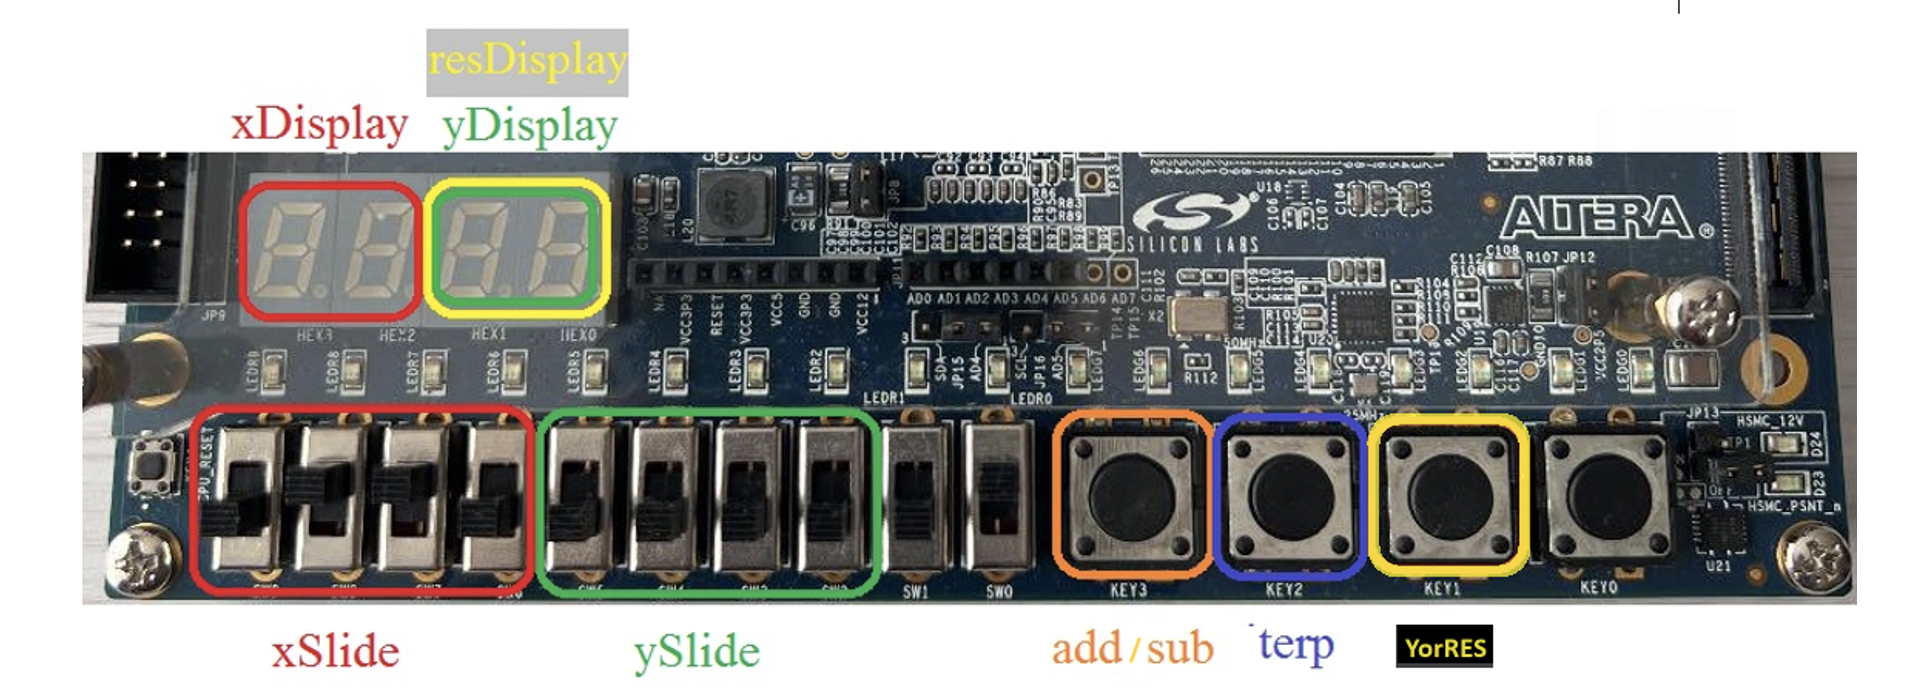
\includegraphics{ image1.png}
\caption{The input and output of the calculator digital circuit.}
\label{fig:calcDevBoard}
\end{figure}

\hypertarget{system-architecture}{%
\section{System Architecture:}\label{system-architecture}}

The system architecture shown in Figure~\ref{fig:sysArchCalc} shows the adder subtractor
processing the xSlide and ySlide inputs. The 4-bit x, y and result
values are processed by the sigUnsig box before being displayed on the
7-segment displays. It is now time to turn our attention to this module.

\begin{figure}
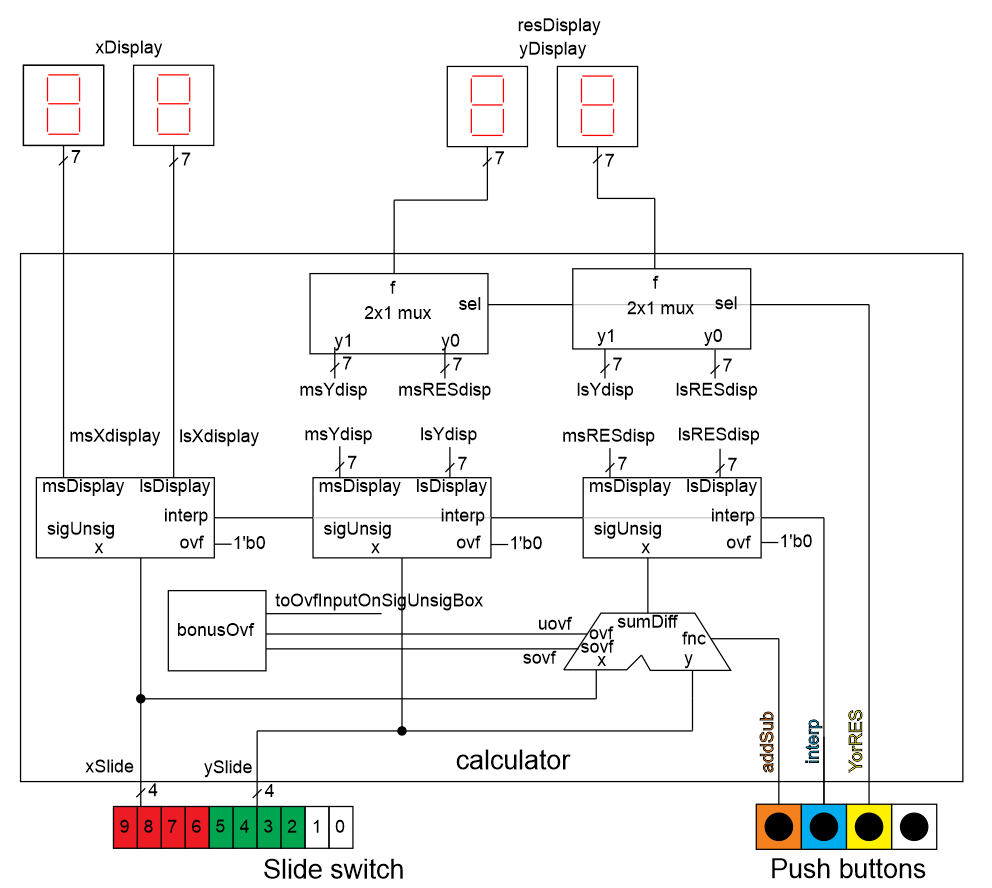
\includegraphics[width=4.43476in,height=3.96969in]{ image2.png}
\caption{The system architecture of the calculator.}
\label{fig:sysArchCalc}
\end{figure}

\hypertarget{sigunsign-module}{%
\section{sigUnsign Module:}\label{sigunsign-module}}

The significant design problem in today's lab comes in this section,
building the sigUnsig module. This module takes in a 4-bit value and
displays a 2-digit signed or unsigned representation on a pair of
7-segment displays. Before we go into the internal organization of this
module, look at its module declaration in Listing 1.

The 4-bit input \emph{x} is interpreted as either signed (2's complement
value) when \emph{interp = 1} or unsigned (regular binary number) when
\emph{interp = 0}. The interpreted value is displayed on the pair of
7-segment display with the tens-digit, blank, or minus sign being
displayed by \emph{msDisplay} and the units digit being displayed by
\emph{lsDisplay}. If the \emph{ovf} input equals 1, the conversion is
overruled and both displays show ``X'' (which looks a lot like a capital
letter ``H''). Because we will need it in the next section, Figure~\ref{fig:calcSevenSeg} is
the logical arrangements of segments in a 7-segment display. Remember
that the segments are active low, meaning a logic 0 illuminates a
segment. Thus, the 7-bit code 7'b0100100 illuminates the pattern ``2''.

\begin{figure}
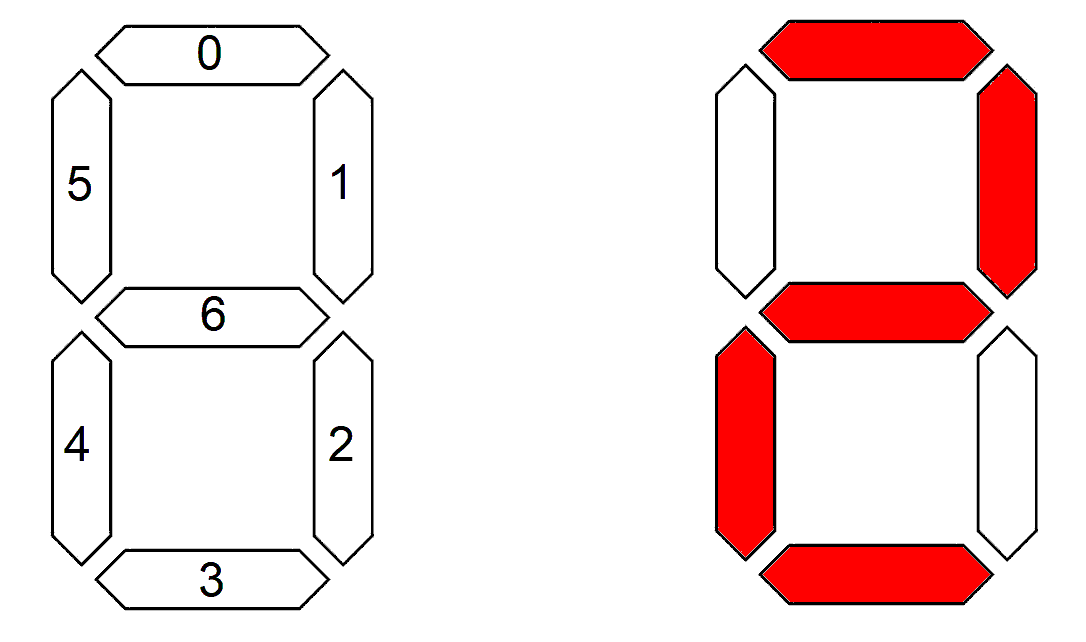
\includegraphics[width=2.60833in,height=1.54375in]{ image3.png}
\caption{The logical arrangements of the segments in a 7-segment display.}
\label{fig:calcSevenSeg}
\end{figure}

Let's start the design of the signUnsig module by looking at the
high-level input/output of the module by completing Table 1. Do this by
filling in the segments of the 7-segment displays that are illuminated
for each of the inputs. Then write the binary and hexadecimal value to
illuminate those patterns.

\begin{longtable}[]{@{}
  >{\raggedright\arraybackslash}p{(\columnwidth - 8\tabcolsep) * \real{0.1458}}
  >{\raggedright\arraybackslash}p{(\columnwidth - 8\tabcolsep) * \real{0.3170}}
  >{\raggedright\arraybackslash}p{(\columnwidth - 8\tabcolsep) * \real{0.0745}}
  >{\raggedright\arraybackslash}p{(\columnwidth - 8\tabcolsep) * \real{0.1458}}
  >{\raggedright\arraybackslash}p{(\columnwidth - 8\tabcolsep) * \real{0.3170}}@{}}
\caption{Table 1: For each set of inputs to the signUnsig module,
determine the 7-segment display pattern.}\tabularnewline
\toprule()
\begin{minipage}[b]{\linewidth}\raggedright
Input
\end{minipage} & \begin{minipage}[b]{\linewidth}\raggedright
7-segment pattern
\end{minipage} & \begin{minipage}[b]{\linewidth}\raggedright
\end{minipage} & \begin{minipage}[b]{\linewidth}\raggedright
Input
\end{minipage} & \begin{minipage}[b]{\linewidth}\raggedright
7-segment pattern
\end{minipage} \\
\midrule()
\endfirsthead
\toprule()
\begin{minipage}[b]{\linewidth}\raggedright
Input
\end{minipage} & \begin{minipage}[b]{\linewidth}\raggedright
7-segment pattern
\end{minipage} & \begin{minipage}[b]{\linewidth}\raggedright
\end{minipage} & \begin{minipage}[b]{\linewidth}\raggedright
Input
\end{minipage} & \begin{minipage}[b]{\linewidth}\raggedright
7-segment pattern
\end{minipage} \\
\midrule()
\endhead
4'b0010

interp = 1

ovf = 0 &
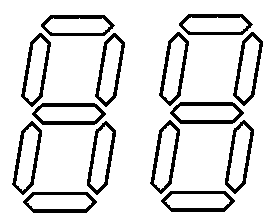
\includegraphics{ image4.png}

msDisplay = 7'b

lsDisplay = 7'b & & 4'b0111

interp = 0

ovf = 0 &
\includegraphics{ image4.png}

msDisplay = 7'b

lsDisplay =7'b \\
4'b1100

interp = 0

ovf = 0 &
\includegraphics{ image5.png}

msDisplay = 7'b1111001 = 7'h79

lsDisplay =7'b0100100 = 7'h24 & & 4'b1000

interp = 1

ovf = 0 &
\includegraphics{ image4.png}

msDisplay = 7'b

lsDisplay =7'b \\
4'b1100

interp = 1

ovf = 0 &
\includegraphics{ image4.png}

msDisplay = 7'b

lsDisplay =7'b & & 4'b1010

interp = 1

ovf = 1 &
\includegraphics{ image4.png}

msDisplay = 7'b

lsDisplay = 7'b \\
\bottomrule()
\end{longtable}

In order to better understand the output from the signUnsig box,
complete Table 2 by filling in the values of \emph{msDisplay} and
\emph{lsDisplay} for a signed and unsigned interpretation -- assume that
\emph{ovf}=0 while completing this table. If the interpreted value is
positive and a single digit then leave \emph{msDisplay} blank. If the
interpreted value is negative then assign \emph{msDisplay} ``-``. If the
interpreted value is greater than 10, assign \emph{msDisplay} ``1''.

For example, let the 4-bit input x equal to 4'b1100. If x is interpreted
as unsigned then its value is 12. In this case your hardware should
assign \emph{msDisplay} ``1'' and \emph{lsDisplay} ``2''. If x is
interpreted as a signed value, the 7-segment displays should show -4, by
assigning \emph{msDisplay} ``-'' and \emph{lsDisplay} ``4''. Complete
the remaining rows of the table.

\begin{longtable}[]{@{}
  >{\raggedright\arraybackslash}p{(\columnwidth - 8\tabcolsep) * \real{0.1999}}
  >{\raggedright\arraybackslash}p{(\columnwidth - 8\tabcolsep) * \real{0.2000}}
  >{\raggedright\arraybackslash}p{(\columnwidth - 8\tabcolsep) * \real{0.2000}}
  >{\raggedright\arraybackslash}p{(\columnwidth - 8\tabcolsep) * \real{0.2000}}
  >{\raggedright\arraybackslash}p{(\columnwidth - 8\tabcolsep) * \real{0.2000}}@{}}
\caption{Table 2: The output of the sigUnsig module when
ovf=0.}\tabularnewline
\toprule()
\multirow{2}{*}{\begin{minipage}[b]{\linewidth}\raggedright
4-bit input x
\end{minipage}} &
\multicolumn{2}{>{\raggedright\arraybackslash}p{(\columnwidth - 8\tabcolsep) * \real{0.4000} + 2\tabcolsep}}{%
\begin{minipage}[b]{\linewidth}\raggedright
\emph{interp = 0} Unsigned
\end{minipage}} &
\multicolumn{2}{>{\raggedright\arraybackslash}p{(\columnwidth - 8\tabcolsep) * \real{0.4000} + 2\tabcolsep}@{}}{%
\begin{minipage}[b]{\linewidth}\raggedright
\emph{interp = 1} Signed
\end{minipage}} \\
& \begin{minipage}[b]{\linewidth}\raggedright
msDisplay
\end{minipage} & \begin{minipage}[b]{\linewidth}\raggedright
lsDisplay
\end{minipage} & \begin{minipage}[b]{\linewidth}\raggedright
msDisplay
\end{minipage} & \begin{minipage}[b]{\linewidth}\raggedright
lsDisplay
\end{minipage} \\
\midrule()
\endfirsthead
\toprule()
\multirow{2}{*}{\begin{minipage}[b]{\linewidth}\raggedright
4-bit input x
\end{minipage}} &
\multicolumn{2}{>{\raggedright\arraybackslash}p{(\columnwidth - 8\tabcolsep) * \real{0.4000} + 2\tabcolsep}}{%
\begin{minipage}[b]{\linewidth}\raggedright
\emph{interp = 0} Unsigned
\end{minipage}} &
\multicolumn{2}{>{\raggedright\arraybackslash}p{(\columnwidth - 8\tabcolsep) * \real{0.4000} + 2\tabcolsep}@{}}{%
\begin{minipage}[b]{\linewidth}\raggedright
\emph{interp = 1} Signed
\end{minipage}} \\
& \begin{minipage}[b]{\linewidth}\raggedright
msDisplay
\end{minipage} & \begin{minipage}[b]{\linewidth}\raggedright
lsDisplay
\end{minipage} & \begin{minipage}[b]{\linewidth}\raggedright
msDisplay
\end{minipage} & \begin{minipage}[b]{\linewidth}\raggedright
lsDisplay
\end{minipage} \\
\midrule()
\endhead
4'b0000 & blank & 0 & blank & 0 \\
4'b0001 & & & & \\
4'b0010 & & & & \\
4'b0011 & & & & \\
4'b0100 & & & & \\
4'b0101 & & & & \\
4'b0110 & & & & \\
4'b0111 & & & & \\
4'b1000 & & & & \\
4'b1001 & & & & \\
4'b1010 & & & & \\
4'b1011 & & & & \\
4'b1100 & 1 & 2 & - & 4 \\
4'b1101 & & & & \\
4'b1110 & & & & \\
4'b1111 & & & & \\
\bottomrule()
\end{longtable}

Note, when there is overflow, you should assign both the
\emph{msDisplay} and \emph{lsDisplay} ``X''.

You will assign the \emph{msDisplay} output one of four values (three
from Table 2 and the ``X'' for overflow) using a 4:1 mux that is
provided to you on Canvas. You will arrange the inputs to this mux using
the logic that you will complete in Listing 2. Note that the four data
inputs to this mux (y0, y1, y2, y3) are constants; the inputs to this
mux do not depend on x.

You will assign the \emph{lsDisplay} output one of four values (three
from Table 2 and the ``X'' for overflow) using a 4:1 mux that is
provided to you on Canvas. You will arrange the inputs to this mux using
the logic that you will complete in Listing 2. Some of the data inputs
to the mux depend on x. For example, if interp = 1 (signed) and if x is
less than 0, then \emph{lsDisplay} should show the 2's complement of x
(and \emph{msDisplay} should display ``-``). Instead of flipping the
bits and adding 1, you should form the negative of x by subtracting x
from 0. On the other hand, if interp = 0 (unsigned) and if x is greater
than or equal to 10, then \emph{lsDisplay} should show the units digit
of x (and \emph{msDisplay} should display ``1``). Form this units digit
by subtracting 10 from x.

Complete the code in Listing 2. You can assign the value blank, -,
constants, x, or a function of x as needed. Note that this code is NOT
to be used in your actual code for this lab.

Now we are ready to put the pieces of the sigUnsig module together. The
building blocks in Figure 4 are captured in the organization described
by Listing 2, along with some extra hardware.

\includegraphics[width=3.21667in,height=2.75417in]{ image6.png}

Figure 4: The internal architecture of the signUnsig module.

You are responsible for connecting the inputs of the 4:1 mux and adder
subtractors using the logic described in Listing 2. To help you do this,
first complete Table 3. Take notice of the comments in the Listing 2 to
determine which data inputs to associate with each of the muxes 4 data
inputs. You should associate the overflow case with the y3 input.

\begin{longtable}[]{@{}
  >{\raggedright\arraybackslash}p{(\columnwidth - 8\tabcolsep) * \real{0.1999}}
  >{\raggedright\arraybackslash}p{(\columnwidth - 8\tabcolsep) * \real{0.2000}}
  >{\raggedright\arraybackslash}p{(\columnwidth - 8\tabcolsep) * \real{0.2000}}
  >{\raggedright\arraybackslash}p{(\columnwidth - 8\tabcolsep) * \real{0.2000}}
  >{\raggedright\arraybackslash}p{(\columnwidth - 8\tabcolsep) * \real{0.2000}}@{}}
\caption{Table 3: The input values to the 4:1 muxes in Figure
4.}\tabularnewline
\toprule()
\begin{minipage}[b]{\linewidth}\raggedright
input
\end{minipage} & \begin{minipage}[b]{\linewidth}\raggedright
y3
\end{minipage} & \begin{minipage}[b]{\linewidth}\raggedright
y2
\end{minipage} & \begin{minipage}[b]{\linewidth}\raggedright
y1
\end{minipage} & \begin{minipage}[b]{\linewidth}\raggedright
y0
\end{minipage} \\
\midrule()
\endfirsthead
\toprule()
\begin{minipage}[b]{\linewidth}\raggedright
input
\end{minipage} & \begin{minipage}[b]{\linewidth}\raggedright
y3
\end{minipage} & \begin{minipage}[b]{\linewidth}\raggedright
y2
\end{minipage} & \begin{minipage}[b]{\linewidth}\raggedright
y1
\end{minipage} & \begin{minipage}[b]{\linewidth}\raggedright
y0
\end{minipage} \\
\midrule()
\endhead
digSel & 2'b11 & & & \\
msDisplay & ``X'' & & 1 & \\
lsDisplay & & & & x \\
\bottomrule()
\end{longtable}

In addition, you should add the following to Figure 4:

\begin{itemize}
\item
  Wire the inputs of the comparator to determine to generate a signal
  xGE10 which is logic 1 when x is greater than or equal to 10.
\item
  Wire the inputs of the adder subtractor according to Table 3.
\item
  Wire the input of the rightmost hexToSevenSeg .
\end{itemize}

The last step in building this module is to describe the behavior of the
glueLogic box. This function chooses which input of the 4 mux inputs to
route to the output. Before you do this, you will need to create a
signal \emph{sign} which equals 1 when x represents a negative value
(when interpreted as a signed value) and equals to 0 when x represents a
positive value (when interpreted as a signed value). Logically speaking,
this is a trivial operation -- it does not require any logic gates.

Now, we can examine the contents of the glueLogic box. Do this by
completing the truth table in Table 4.

\begin{longtable}[]{@{}
  >{\raggedright\arraybackslash}p{(\columnwidth - 8\tabcolsep) * \real{0.1999}}
  >{\raggedright\arraybackslash}p{(\columnwidth - 8\tabcolsep) * \real{0.2000}}
  >{\raggedright\arraybackslash}p{(\columnwidth - 8\tabcolsep) * \real{0.2000}}
  >{\raggedright\arraybackslash}p{(\columnwidth - 8\tabcolsep) * \real{0.2000}}
  >{\raggedright\arraybackslash}p{(\columnwidth - 8\tabcolsep) * \real{0.2000}}@{}}
\caption{Table 4: Truth table for the glueLogic box.}\tabularnewline
\toprule()
\begin{minipage}[b]{\linewidth}\raggedright
ovf
\end{minipage} & \begin{minipage}[b]{\linewidth}\raggedright
interp
\end{minipage} & \begin{minipage}[b]{\linewidth}\raggedright
sign
\end{minipage} & \begin{minipage}[b]{\linewidth}\raggedright
xGE10
\end{minipage} & \begin{minipage}[b]{\linewidth}\raggedright
digSel
\end{minipage} \\
\midrule()
\endfirsthead
\toprule()
\begin{minipage}[b]{\linewidth}\raggedright
ovf
\end{minipage} & \begin{minipage}[b]{\linewidth}\raggedright
interp
\end{minipage} & \begin{minipage}[b]{\linewidth}\raggedright
sign
\end{minipage} & \begin{minipage}[b]{\linewidth}\raggedright
xGE10
\end{minipage} & \begin{minipage}[b]{\linewidth}\raggedright
digSel
\end{minipage} \\
\midrule()
\endhead
1 & x & x & x & \\
0 & 0 & x & 0 & \\
0 & 0 & x & 1 & \\
0 & 1 & 0 & x & \\
0 & 1 & 1 & x & \\
\bottomrule()
\end{longtable}

1

It would make sense to use an always case statement to realize the logic
in Listing 2. However, an always case statement requires each of the 16
difference cases to be explicitly enumerated. However, the truth table
in Listing 2 is most efficiently described using don't cares in the
input. Fortunately, the always/casez variation (note the ``z'' at the
end of ``case'') allows don't cares in the input in the form of ``?''.
For example, for the second row in Listing 2, the \{ovf, interp, sign,
xGE10\} vector has don't cares for the \emph{sign} value. Therefore, the
case for this row is 4'b01?0. \uline{It is imperative that you include a
``default'' case whenever you use a always/case statement.} This
combination of cases is shown in Listing 3.

\protect\hypertarget{sigUnsign_Verilog}{}{}The Verilog code for the
signUnsig module consists of 8 instantiation statements and an
always/casez statement. For this module, I want you to:

\begin{itemize}
\item
  Use the module declaration given in Listing 1.
\item
  Use the module definitions for

  \begin{itemize}
  \item
    Generic Mux4x1 posted on this lab's Canvas folder
  \item
    sevenSegment created in lab 02
  \item
    genericAdderSubtractor posted on a previous lab's Canvas folder
  \item
    genericComparator posted on a previous lab's Canvas folder
  \end{itemize}
\item
  Use localparm to give names to the 7-bit constant patterns (fill in
  the values for x).

  \begin{itemize}
  \item
    localparam {[}6:0{]} displayBlank = 7'bxxxxxxx;
  \item
    localparam {[}6:0{]} displayOne = 7'bxxxxxxx;
  \item
    localparam {[}6:0{]} displayMinus = 7'bxxxxxxx;
  \item
    localparam {[}6:0{]} displayX = 7'bxxxxxxx;
  \end{itemize}
\item
  Provide meaningful names to the wires in the module.
\item
  Properly tab-indent your code

  \begin{itemize}
  \item
    Single level for wire declarations
  \item
    Single level for component instantiations
  \item
    Two levels for casez statement
  \item
    Three levels for casez values
  \end{itemize}
\end{itemize}

\hypertarget{section}{%
\section{}\label{section}}

\hypertarget{bonus-ovf-logic}{%
\section{Bonus Ovf Logic:}\label{bonus-ovf-logic}}

The default configuration of the system architecture ignores any
overflow generated by the adder subtractor. If you choose, you may
implement the logic necessary to determine if overflow occurs in the
selected interpretation. In order to receive credit, your circuit needs
to work under \uline{all combination} of addSub and interp. Overflow for
unsigned subtraction will require some careful analysis.

Your solution should have 2 LEDs, one for signed and one for unsigned.
The unsigned overflow LED should illuminate when overflow will occur if
the numbers are interpreted as unsigned numbers. The signed overflow LED
is on when an overflow will occur if the numbers are interpreted as
two's complement numbers.

For example, if the x and y inputs are 1001 and the operation is
addition, then both signed and unsigned LEDs will illuminate.

\hypertarget{pin-assignment}{%
\section{Pin Assignment:}\label{pin-assignment}}

Use the image of the development board in Figure~\ref{fig:calcDevBoard} in and the
information in the Cyclone V GX Kit User Manual (posted on the class web
page) to determine the FPGA pins associated with the input and output
devices used by the calculator module

\begin{longtable}[]{@{}
  >{\raggedright\arraybackslash}p{(\columnwidth - 8\tabcolsep) * \real{0.1436}}
  >{\raggedright\arraybackslash}p{(\columnwidth - 8\tabcolsep) * \real{0.1829}}
  >{\raggedright\arraybackslash}p{(\columnwidth - 8\tabcolsep) * \real{0.1665}}
  >{\raggedright\arraybackslash}p{(\columnwidth - 8\tabcolsep) * \real{0.2621}}
  >{\raggedright\arraybackslash}p{(\columnwidth - 8\tabcolsep) * \real{0.2448}}@{}}
\toprule()
\begin{minipage}[b]{\linewidth}\raggedright
Segment
\end{minipage} & \begin{minipage}[b]{\linewidth}\raggedright
msXdisplay
\end{minipage} & \begin{minipage}[b]{\linewidth}\raggedright
lsXdisplay
\end{minipage} & \begin{minipage}[b]{\linewidth}\raggedright
msYorRESdisplay
\end{minipage} & \begin{minipage}[b]{\linewidth}\raggedright
lsYorRESdisplay
\end{minipage} \\
\midrule()
\endhead
seg{[}6{]} & & & & \\
seg{[}5{]} & & & & \\
seg{[}4{]} & & & & \\
seg{[}3{]} & & & & \\
seg{[}2{]} & & & & \\
seg{[}1{]} & & & & \\
seg{[}0{]} & & & & \\
\bottomrule()
\end{longtable}

\begin{longtable}[]{@{}
  >{\raggedright\arraybackslash}p{(\columnwidth - 4\tabcolsep) * \real{0.3397}}
  >{\raggedright\arraybackslash}p{(\columnwidth - 4\tabcolsep) * \real{0.3278}}
  >{\raggedright\arraybackslash}p{(\columnwidth - 4\tabcolsep) * \real{0.3325}}@{}}
\toprule()
\begin{minipage}[b]{\linewidth}\raggedright
\end{minipage} & \begin{minipage}[b]{\linewidth}\raggedright
x
\end{minipage} & \begin{minipage}[b]{\linewidth}\raggedright
y
\end{minipage} \\
\midrule()
\endhead
slide{[}3{]} & & \\
slide{[}2{]} & & \\
slide{[}1{]} & & \\
slide{[}0{]} & & \\
\bottomrule()
\end{longtable}

\begin{longtable}[]{@{}
  >{\raggedright\arraybackslash}p{(\columnwidth - 4\tabcolsep) * \real{0.3334}}
  >{\raggedright\arraybackslash}p{(\columnwidth - 4\tabcolsep) * \real{0.3334}}
  >{\raggedright\arraybackslash}p{(\columnwidth - 4\tabcolsep) * \real{0.3333}}@{}}
\toprule()
\begin{minipage}[b]{\linewidth}\raggedright
\hypertarget{yorres}{%
\section{YorRES}\label{yorres}}
\end{minipage} & \begin{minipage}[b]{\linewidth}\raggedright
Key{[}1{]}
\end{minipage} & \begin{minipage}[b]{\linewidth}\raggedright
\end{minipage} \\
\midrule()
\endhead
\begin{minipage}[t]{\linewidth}\raggedright
\hypertarget{interp}{%
\section{interp}\label{interp}}
\end{minipage} & Key{[}2{]} & \\
\begin{minipage}[t]{\linewidth}\raggedright
\hypertarget{addsub}{%
\section{addSub}\label{addsub}}
\end{minipage} & Key{[}3{]} & \\
\bottomrule()
\end{longtable}

\textbf{Turn in:}

You may work in teams of at most two. Make a record of your response to
the items below and turn them in a single copy as your team's solution
on Canvas using the instructions posted there. Include the names of both
team members at the top of your solutions. Use complete English
sentences to introduce what each of the following listed items (below)
is and how it was derived. In addition to this submission, you will be
expected to demonstrate your circuit at the beginning of your lab
section next week.

\hypertarget{signunsig-module}{%
\section{\texorpdfstring{signUnsig Module:
}{signUnsig Module: }}\label{signunsig-module}}

\begin{itemize}
\item
  Complete Table 1.
\item
  Complete Table 2.
\item
  Complete the code in Listing 2.
\item
  Complete Figure 4, including:

  \begin{itemize}
  \item
    Constant values on inputs of 4:1 mux
  \item
    Constant value on the input of the right-most hexToSeventSeg
  \item
    Value on the input of the adder subtractors
  \item
    Values on the input of the comparator
  \end{itemize}
\item
  Complete Table 3.
\item
  Complete Table 4.
\item
  \protect\hyperlink{sigUnsign_Verilog}{Verilog code for the body of the
  sigUnsig module} (courier 8-point font single spaced), leave out
  header comments.
\item
  Run the testbench for the sigUnsig module provided on Canvas. Produce
  a timing diagram with the following characteristics. Zoom to fill the
  available horizontal space with the waveform. Color inputs green and
  outputs red. Order the traces from top to bottom as

  \begin{itemize}
  \item
    x radix unsigned Green trace
  \item
    xMinus10 radix unsigned Green trace
  \item
    x radix decimal Cyan trace
  \item
    negativeX radix decimal Cyan trace
  \item
    interp default Green trace
  \item
    ovf default Green trace
  \item
    digSel radix unsigned Yellow trace
  \item
    xGE10 default Yellow trace
  \item
    msDisplay radix hex Red trace
  \item
    lsDisplay radix hex Red trace
  \end{itemize}
\end{itemize}

I do not want the signals from the testbench, but rather the signals
from inside the sigUnsig module. You can do this in sigUnsig, by
expanding the sigUnsig\_tb instance in the left ModelSim pane and
selecting ``uut''. Since uut is an instance of the sigUnsig module, all
the signals accessible in the sigUnsig module are shown in the center
Object. You can add duplicates of signals by repeating the drag-and-drop
operation.

Your completed timing diagram should look something like the following.

\includegraphics[width=7.15208in,height=1.87153in]{ image7.png}

\textbf{Pin Assignment:}

Complete all three pin assignment tables.


\chapter{Cellular Automata}
\label{chapter:cellAuto}
\graphicspath{ {./Lab07CellularAutomata/Fig} }

\section{Outcomes and Objectives}

The outcome of this lab is to instantiate a 1-dimensional 
cellular automata using D-Flip Flops and combinational logic.
Through this process you will achieve the following
learning objectives.
\begin{itemize}
	\item \Paste{bok:BasicMemoryElements}
	\item \Paste{bok:BME_Timing}	
	\item \Paste{VER:Module}
	\item \Paste{HDL:Synthesis}			
\end{itemize}



\section{1-dimensional cellular automata}

A common research theme in intelligent systems is emergent complexity.
This is the idea that complex behavior can arise from an interconnected
arrangement of simple processing elements following simple rules. 

\subsection{Theory: Cellular Automata}
As a testbench for this idea, Stephen Wolfram\footnote{Wolfram, S.
  "Statistical Mechanics of Cellular Automata." Rev. Mod. Phys. 55,
  601-644, 1983.} explored emergent complexity in a 1-dimensional
cellular automata (1-DCA) network. A 1-DCA is an array of processing
elements, each of which has one of two states (called alive and dead)
and is interconnected to the neighbors immediately to its left and
right. The next state of each processing element depends on its current
state and the current state of the neighbors to its immediate left and
right. Let's explore the evolution of a 1-DCA using the setup shown in
Figure~\ref{fig:exampleCA}, note that cells which are alive are shaded and cells which are
dead, white.

\begin{figure}[ht]
\includegraphics{image1.png}
\caption{A 1-DCA consisting of 8 processing elements. Alive cells are
shaded grey, dead white.}
\label{fig:exampleCA}
\end{figure}

Let's examine the next state of the 1-DCA shown in Figure~\ref{fig:exampleCA} 
using the rule where:

\begin{itemize}
\item
  An alive cell stays alive when exactly 1 of its neighbors is alive,
  else it dies.
\item
  A dead cell comes alive when exactly 1 of its neighbors is alive, else
  it stays dead.
\end{itemize}

Complete the unfilled entries in Table~\ref{table:caNextState} using the initial state shown
in Figure~\ref{fig:exampleCA} and the rule above. We will imagine that our processing
elements are placed on a ring. This implies that the left neighbor of
processing element C7 is C0 and the right neighbor of processing element
of C0 is C7.

\begin{longtable}[]{@{}
|  >{\raggedright\arraybackslash}p{(\columnwidth - 6\tabcolsep) * \real{0.1683}}|
  >{\raggedright\arraybackslash}p{(\columnwidth - 6\tabcolsep) * \real{0.2772}}|
  >{\raggedright\arraybackslash}p{(\columnwidth - 6\tabcolsep) * \real{0.3198}}|
  >{\raggedright\arraybackslash}p{(\columnwidth - 6\tabcolsep) * \real{0.2347}}|@{}}
\caption{The next state of a processing element depends on the
current state and the number of alive neighbors.} \label{table:caNextState} \tabularnewline
\toprule()
\begin{minipage}[b]{\linewidth}\raggedright
Cell
\end{minipage} & \begin{minipage}[b]{\linewidth}\raggedright
Current State
\end{minipage} & \begin{minipage}[b]{\linewidth}\raggedright
\# Alive neighbors
\end{minipage} & \begin{minipage}[b]{\linewidth}\raggedright
Next State
\end{minipage} \\
\midrule()
\endfirsthead
\toprule()
\begin{minipage}[b]{\linewidth}\raggedright
Cell
\end{minipage} & \begin{minipage}[b]{\linewidth}\raggedright
Current State
\end{minipage} & \begin{minipage}[b]{\linewidth}\raggedright
\# Alive neighbors
\end{minipage} & \begin{minipage}[b]{\linewidth}\raggedright
Next State
\end{minipage} \\
\midrule()
\endhead
C0 & Dead & & \\ \hline
C1 & Dead & & \\ \hline
C2 & Alive & 0 & \\ \hline
C3 & Dead & & \\ \hline
C4 & Alive & & Alive \\ \hline
C5 & Alive & & \\ \hline
C6 & Dead & & \\ \hline
C7 & Alive & & \\
\bottomrule()
\end{longtable}

You are going to build a digital system to calculate the next state of a
9-element array of processing elements. In order to do this, you will
need a way to easily specify the rule used to determine the next state
of a cell because you are going to be able to change it. Before doing
this let's agree to associate the value of 1 for an alive cell and
illustrate it as a filled black square and associate the value 0 with a
dead cell and will illustrate it as an empty square.

We will formalize the next state rule by enumerating the next state of a
cell for every configuration of its current state and its neighbor's
state. Since a cell and it's two neighbors can each have two states,
there are a total of 8 configurations. As an example, I've graphically
illustrated the rule used in our previous example, in Figure~\ref{fig:caRule}. This
arrangement shows the 8 configurations arranged so the binary code of
the current states goes from 3'b000 at right to 3'b111 at left. The next
state for each configuration is shown below the current state
configuration.

\begin{figure}[ht]
\includegraphics{image2.png}
\caption{The next state of the center cell depends on the current state
of a cell and its neighbors.}
\label{fig:caRule}
\end{figure}


\pagebreak


As an example, let's look at the 4\textsuperscript{th} from left
arrangement, outlined in red. In the top row of this arrangement, the
center cell is dead and one of its neighbor's is alive.  Note that this
configuration has binary code 3'b100. Using the rule used to complete
Table~\ref{table:caNextState}, the next state of this cell is alive, shown black. The next
state value is placed below each configuration and the collection forms
an 8-bit number 8'b01011010, which when interpreted as a decimal value
is equal to 90. We will call the rule used to update the cells in Table
1, rule 90.

The fact that we are numbering this rule, implies that there may be
others. In fact, there are 256 different rule sets. You can create new
rules by substituting new combinations of alive and dead states for each
next states shown in Figure~\ref{fig:caRule}. Not all rules generate interesting
behavior. For example, rule 0 immediately kills any and all alive cells
producing a desert. Stephen Wolfram explored every combination of rules
and characterized the resulting patterns into one of four classes
depending on their sophistication. Wolfram illustrated this
sophistication by arranging successive iterations of the 1-DCA as rows.
As an example, if you start with a single alive cell and run Rule 90
over many iterations, drawing iteration below its predecessor, you get
the image shown in Figure~\ref{fig:caEvolution}. Some of you may recognize this figure as
the Sierpiński Triangle\footnote{\url{https://en.wikipedia.org/wiki/Sierpi\%C5\%84ski_triangle}},
an elementary fractal.

\begin{figure}[ht]
\includegraphics[width=0.5\paperwidth]{image3.png}
\caption{The evolution of a single alive cell (shown at top) under Rule 90.}
\label{fig:caEvolution}
\end{figure}

You now have all the information and terminology you need to build a
digital system to compute the next state of a 1-DCA, so let's get to it.

\subsection{Implementation: Cellular Automata}

You will use the inputs and outputs shown in Figure~\ref{fig:caDevBoard} to realize a
9 cell 1-DCA. I chose 9 cells so that we could have a unique center
cell. Each of the 9 \textbf{Initial State} slide switches corresponds to
one of the 9 cells. In order to set the state of the cells the
\textbf{loadRun} slide switch must be in the down position. Moving the
Initial State up/down will set its corresponding cell to 1/0
respectively when the array is clocked. A cell that is alive will
illuminate its associated \textbf{CurrentState} LED. After the initial
state of the cells is set, you should move the \textbf{loadRun} slide
switch up and set the 8-bit rule value using the \textbf{Rule} slide
switches. Every time that the array is clocked, the
\textbf{CurrentState} LEDs will show the array.

\begin{figure}[ht]
\includegraphics{image4.png}
\caption{The input and output of the 1D cellular automata.}
\label{fig:caDevBoard}
\end{figure}

The \textbf{reset} button will reset the state of all the cells to 0 --
dead. The clock is a bit more complex than you might expect because of
switch bouncing. When you press one of the push buttons on the Cyclone V
GX board, the signal generated may not transition smoothly from logic 0
to logic 1. Instead, it may do something like that shown in Figure~\ref{fig:caSwitchBounce}. In
this figure, a single press of the button created four transitions from
logic 0 to logic 1. This happens because the metal contact attached to
the round plastic button physically bounced off the metal contacts
attached to the body of the button. This is more prone to happen if you
quickly and sharply jab at the button.

\begin{figure}[ht]
\begin{tabular}{ccc }
\includegraphics[width=0.3\paperwidth]{image5.png} &  & \includegraphics{image6.png} \\
A  & & B \\ 
\end{tabular}
\caption{A) Switch bouncing makes generating a single clock edge problematic.
B) The organization of the SR latch to run the clock requires
inverters in the sClk and rClk inputs and an SR latch to help remove
signal bouncing.}
\label{fig:caSwitchBounce}
\end{figure}

However, even the most casual of presses may generate switch bouncing,
so you are going to design a digital circuit (an SR latch) to prevent
this from happening. When you press the \textbf{sClk} button, the clock
signal will be set. When you press the \textbf{rClk} button, the clk
signal will be reset. If the \textbf{sClk} or bounces, the clock line
will not bounce because this switch bounce will only cause the clk line
to be repeatedly be set when it already set. Likewise, with the
\textbf{rClk} signal repeatedly resetting the clk signal if
\textbf{rClk} bounces. Finally, in order for you to know the state of
the clk, its logic level is display on the \textbf{clk} LED.

Since the buttons driving the rClk and sClk signals are logic 0 when
pressed, you will want to invert these two signals before feeding them
into the SR latch as shown in Figure~\ref{fig:caSwitchBounce}B. Thus, to 
toggle the clock signal
you will press/release the sClk button to set clk to 1. Then
press/release the rClk button to clear the clk to 0. The back to sClk,
etc\ldots{}



\section{System Architecture}

The system architecture shown in Figure~\ref{fig:caSysArch} shows the overall organization
of the cellular automata. Slide switches {[}0-7{]} are used as initial
state when the loadRun slide switch is set to 0. When the loadRun slide
switch is set to 1, slide switches {[}0-7{]} are used as the evolution
rule. The clock is generated by the SR latch whose inputs are sClk and
rClk. The state of the cells are displayed on the 9 red LEDs. The
processing elements forming the array are called singleCell and
discussed in the next section.

\begin{figure}[ht]
\includegraphics{image7.png}
\caption{The system architecture of the cellularAutomata. Due to tight
spacing, only the n inputs to cell8 and cell2 are shown.}
\label{fig:caSysArch}
\end{figure}

\protect\hypertarget{cellularAutomata_verilog}{}{}The Verilog code for
the cellularAutomata has been partially provided to you. You will need
to complete the missing pieces. For this module:

\begin{itemize}
\item
  Use the cellularAutomata.v file provided in the Canvas folder as the
  starting point.
\item
  Make a vector for the \emph{rule} and \emph{initialState} from the
  \emph{slideSwitches} input vector.
\item
  Make a 3-bit vector input for each singleCell by appending its current
  state to the two neighbors current state using the ``\{\}'' operators.
  See the singleCell module for more information.
\item
  Connect the ends of the CA together

  \begin{itemize}
  \item
    Make cell 8 have cell 0 as its ``left'' neighbor in Figure~\ref{fig:caSysArch}
  \item
    Make cell 0 have cell 8 as its ``right'' neighbor in Figure~\ref{fig:caSysArch}
  \end{itemize}
\item
  Use cross-couples NORs and a pair of inverters to realize the SR-latch. This means that you
  should have two lines of Verilog Code for the SR-latch, both starting
  with ``assign''.
\item
  You are encouraged to use the generate statement to instantiate
  singleCell 1-7. Due the ring architecture, you will need to
  instantiate cells 0 and 7 individually. For an example of the generate
  statement, look at the adderSubtractor provided to you in a previous
  lab.
\end{itemize}


\section{Module: singleCell}

The significant design problem in today's lab comes in this section,
building the singleCell module. The module interface for the singleCell
module in Figure~\ref{fig:caSysArch} used some shorthand for the single names due to the
space constraints. The internal organization and module interface for
the singleCell module is shown in Figure~\ref{fig:caSingleCell}. For example, the output
currentState in this figure was called Q in Figure~\ref{fig:caSysArch}. You should be able
to decipher the rest of the signal abbreviations used in Figure~\ref{fig:caSysArch}.

\begin{figure}[ht]
\includegraphics[width=0.3\paperwidth]{image8.png}
\caption{The architecture and module interface for the singleCell module.}
\label{fig:caSingleCell}
\end{figure}

The most complex portion of logic in the singleCell module is the box
labeled ``nextState''. This circuit has 11-bits of input.  While it may
seem a bit daunting at first, the Verilog code to realize this function
is pretty straightforward when you have the right perspective. Table~\ref{table:caInOutSingleCell}
lists all the combination of state for a cell and its 2 neighbors in the
left column (n+ is the state of the neighbor to the left, n the state of
the cell itself, and n- the state to the right). These 8 combinations
are the case values in the always/case statement for the nextState
logic. You need to know the output for each of these cases. As an
example, complete the nextState column in Table~\ref{table:caInOutSingleCell} for Rule 90 using the
information in Figure~\ref{fig:caRule}. In the ``Rule bit'' column in Table~\ref{table:caInOutSingleCell},
generalize the nextState column to the bit values in the 8-bit rule
vector that is passed into the singleCell module.

\begin{longtable}[]{@{}
| >{\raggedright\arraybackslash}p{(\columnwidth - 4\tabcolsep) * \real{0.3528}}|
  >{\raggedright\arraybackslash}p{(\columnwidth - 4\tabcolsep) * \real{0.3236}}|
  >{\raggedright\arraybackslash}p{(\columnwidth - 4\tabcolsep) * \real{0.3236}}|@{}}
\caption{The input/output relationship for the nextState
functionality in Figure~\ref{fig:caSingleCell}.}\label{table:caInOutSingleCell}\\ \hline
\toprule()
\{n+, n, n-\} &  nextState & Rule bit \\ 
\midrule()
\endfirsthead
\toprule()
\{n+, n, n-\} &  nextState & Rule bit \\ 
\midrule()
\endhead
3'b000 & & \\ \hline
3'b001 & & \\ \hline
3'b010 & & rule{[}2{]} \\ \hline
3'b011 & & \\ \hline
3'b100 & 1 & \\ \hline
3'b101 & & \\ \hline
3'b110 & & \\ \hline
3'b111 & & \\ 
\bottomrule()
\end{longtable}

\protect\hypertarget{singleCell_verilog}{}{}For the singleCell module, I
want you to:

\begin{itemize}
\item
  Use the singleCell.v file provided in the Canvas folder as the
  starting point.
\item
  Use an always/case statement for the nextState logic
\item
  Use the module definitions for:

  \begin{itemize}
  \item
    Use the genericMux2x1 from a previous lab.
  \item
    Use the dffNegEdge module provided in the Canvas lab folder for this
    lab.
  \end{itemize}
\item
  Provide meaningful names to the wires in the module.
\item
  Properly tab-indent your code

  \begin{itemize}
  \item
    Single level for wire declarations
  \item
    Single level for component instantiations
  \item
    Two levels for case statement
  \item
    Three levels for case values
  \end{itemize}
\end{itemize}

\section{Testbench}
\label{section:caTestbench}

  Run the testbench for the cellularAutomata module provided on Canvas.
  Produce a timing diagram with the following characteristics. Zoom to
  fill the available horizontal space with the waveform. Color inputs
  green and outputs red. Order the traces from top to bottom as

\begin{tabular}{p{4cm}p{4cm}p{4cm}}
signal		& radix				& tracel color \\ \hline
    reset 			& default 			& Blue  \\ 
    rule 			&  unsigned 			& Blue \\ 
    sButton 			& default 		& Green \\ 
    rButton 			& default 		& Green \\ 
    clk 				& default 		& Yellow \\ 
    currentLifeState 	& hex 			& Red \\
  \end{tabular}


Do not use the signals from the testbench, but rather the signals
from inside the cellularAutomata module. You can do this in ModelSim, by
expanding the cellularAutomata\_tb instance in the left ModelSim and
selecting ``uut''. Since uut is an instance of the cellularAutomata
module, all the signals accessible in the cellularAutomata module are
shown in the center Object. You can add signals using a drag-and-drop
operation. Likewise, you can reorder the signals by dragging them. Your
completed timing diagram should look something like Figure~\ref{fig:caTimeDiag}.

\begin{figure}[ht]
\includegraphics{image9.png}
\caption{Partial timing diagram for the cellular automata.}
\label{fig:caTimeDiag}
\end{figure}



\section{Pin-Assignment and Synthesis}

Use the image of the FPGA Board in Figure~\ref{fig:exampleCA} 
and the information
in the C5G User Guide to determine the FPGA pins associated
with the input and output devices used by the cellular automata module.

\begin{longtable}[]{@{}
| >{\raggedright\arraybackslash}p{(\columnwidth - 8\tabcolsep) * \real{0.1986}}|
  >{\raggedright\arraybackslash}p{(\columnwidth - 8\tabcolsep) * \real{0.2067}}|
  >{\raggedright\arraybackslash}p{(\columnwidth - 8\tabcolsep) * \real{0.1935}}|
  >{\raggedright\arraybackslash}p{(\columnwidth - 8\tabcolsep) * \real{0.1954}}|
  >{\raggedright\arraybackslash}p{(\columnwidth - 8\tabcolsep) * \real{0.2058}}|@{}}
   \caption{Pin Assignment for the 1-D calllular automata.}\label{table:cAutomataPinAssignment} \\ \hline
\endfirsthead 
slide{[}9{]} & AE19 & &
Clk

LEDG6 & \\ \hline
slide{[}8{]} & & & led {[}8{]}

LEDR8 & \\ \hline
slide{[}7{]} & & & led {[}7{]} & K8\\ \hline
slide{[}6{]} & & & led {[}6{]} & \\ \hline
slide{[}5{]} & & & led {[}5{]} & \\ \hline
slide{[}4{]} & & & led {[}4{]} & \\ \hline
slide{[}3{]} & & & led {[}3{]} & \\ \hline
slide{[}2{]} & & & led {[}2{]} & \\ \hline
slide{[}1{]} & & & led {[}1{]} & \\ \hline
slide{[}0{]} & & & led {[}0{]}

LEDR0 & \\ 
\bottomrule()
\end{longtable}

\begin{longtable}[]{@{}
| >{\raggedright\arraybackslash}p{(\columnwidth - 4\tabcolsep) * \real{0.3334}}|
  >{\raggedright\arraybackslash}p{(\columnwidth - 4\tabcolsep) * \real{0.3334}}|
  >{\raggedright\arraybackslash}p{(\columnwidth - 4\tabcolsep) * \real{0.3333}}|@{}}
\toprule()
\begin{minipage}[b]{\linewidth}\raggedright
sClk
\end{minipage} & \begin{minipage}[b]{\linewidth}\raggedright
Key{[}3{]}
\end{minipage} & \begin{minipage}[b]{\linewidth}\raggedright
\end{minipage} \\
\midrule()
\endhead
\begin{minipage}[t]{\linewidth}\raggedright
rClk
\end{minipage} & Key{[}2{]} & Y15 \\ \hline
\begin{minipage}[t]{\linewidth}\raggedright
reset
\end{minipage} & Key{[}1{]} & \\ 
\bottomrule()
\end{longtable}

Complete the pin-assignment in Quartus, compile your design and download to the
FGPA development boards.  If you are having difficulty getting your circuit to work
correctly, please refer to Section~\ref{section:caDebugging} for some 
useful debugging tips. 

Once you get your design working, demonstrate it to a member of the 
lab team.  



\section{Turn in}

You may work in teams of at most two. Make a record of your response to
the items below and turn them in a single copy as your team's solution
on Canvas using the instructions posted there. Include the names of both
team members at the top of your solutions. Use complete English
sentences to introduce what each of the following listed items (below)
is and how it was derived. In addition to this submission, you will be
expected to demonstrate your circuit at the beginning of your lab
section next week.

\subsubsection{Cellular Automata Module }

\begin{itemize}
\item
  Complete Table~\ref{table:caNextState}.
\item
  \protect\hyperlink{cellularAutomata_verilog}{Link} Verilog code for
  the body of the cellularAutomata module (courier 8-point font single
  spaced), leave out header comments.
\end{itemize}

\subsubsection{singleCell Module}

\begin{itemize}
\item
  Complete Table~\ref{table:caInOutSingleCell}.
\item
  \protect\hyperlink{singleCell_verilog}{Link} Verilog code for the body
  of the singleCell module (courier 8-point font single spaced), leave
  out header comments.
\end{itemize}

\subsubsection{Testbench}
\begin{itemize}
\item Complete testbench and timing diagram from Section~\ref{section:caTestbench}.
\end{itemize}

\subsubsection{Pin-Assignment and Synthesis}
\begin{itemize}
\item Complete the pin assignment in table~\ref{table:cAutomataPinAssignment}.
\item Demonstrate your completed circuit to a lab team member.
\end{itemize}




\section{Debugging Tips}
\label{section:caDebugging}
To provide you with some examples to run on the Altera boards, the
following table illustrates the evolution of the CA with different
initial conditions and different rules.

\begin{itemize}
\item
  In the left most column contains several different rows

  \begin{itemize}
  \item
    The row labeled ``Rule \#'' is the rule that you will enter on the
    slide switches. The binary code of the rule is provided to make
    setting your dip switches easier.
  \item
    The row labeled ``start'' is the initial load value stored in the
    CA. A value of ``x'' means that the initial load value doesn't
    matter (don't care).
  \item
    The rows labeled ``iteration'' count successive positive edges
    generated by the clock.
  \end{itemize}
\item
  The column labeled
  ``q\textsubscript{8}q\textsubscript{7}q\textsubscript{6}q\textsubscript{5}''
  is the output from the 4 most significant bits of the CA
\item
  The column labeled ``q\textsubscript{4}'' is the output from the
  middle bit of the CA
\item
  The column labeled
  ``q\textsubscript{3}q\textsubscript{2}q\textsubscript{1}q\textsubscript{0}''
  is the output from the 4 least significant bits of the CA
\end{itemize}


\begin{longtable}[]{@{}
|  >{\raggedright\arraybackslash}p{(\columnwidth - 6\tabcolsep) * \real{0.2723}}|
  >{\raggedright\arraybackslash}p{(\columnwidth - 6\tabcolsep) * \real{0.2426}}|
  >{\raggedright\arraybackslash}p{(\columnwidth - 6\tabcolsep) * \real{0.2426}}|
  >{\raggedright\arraybackslash}p{(\columnwidth - 6\tabcolsep) * \real{0.2426}}|@{}} \\ \hline
\endfirsthead
\endhead

\textbf{Rule 0:}

\textbf{0000 0000}  &  q\textsubscript{8}q\textsubscript{7}q\textsubscript{6}q\textsubscript{5}
& q\textsubscript{4} & q\textsubscript{3}q\textsubscript{2}q\textsubscript{1}q\textsubscript{0} \\ \hline
Start: & XXXX & X & XXXX \\ \hline
Final: & 0000 & 0 & 0000 \\ \hline
& & & \\ \hline
\textbf{Rule 255:}

\textbf{1111 1111} & & & \\ \hline
Start: & XXXX & X & XXXX \\ \hline
Final: & 1111 & 1 & 1111 \\ \hline
& & & \\ \hline
\textbf{Rule 90:}

\textbf{0101 1010} & & & \\ \hline
Start: & 0000 & 1 & 0000 \\ \hline
1st Iteration: & 0001 & 0 & 1000 \\ \hline
2nd Iteration: & 0010 & 0 & 0100 \\ \hline
3rd Iteration: & 0101 & 0 & 1010 \\ \hline
4th Iteration: & 1000 & 0 & 0001 \\ \hline
5th Iteration & 1100 & 0 & 0011 \\ \hline
6th Iteration & 0110 & 0 & 0110 \\ \hline
7th Iteration & 1111 & 0 & 1111 \\ \hline
& & & \\ \hline
\textbf{Rule 90:}

\textbf{0101 1010} & & & \\ \hline
Start: & 1011 & 0 & 1101 \\ \hline
1st Iteration: & 1011 & 0 & 1101 \\ \hline
Final: & 1011 & 0 & 1101 \\ \hline
& & & \\ \hline
\textbf{Rule 254:}

\textbf{1111 1110} & & 1111 & 1110 \\ \hline
Start: & 1000 & 0 & 0000 \\ \hline
1st Iteration: & 1100 & 0 & 0001 \\ \hline
2nd Iteration: & 1110 & 0 & 0011 \\ \hline
3rd Iteration: & 1111 & 0 & 0111 \\ \hline
Final: & 1111 & 1 & 1111 \\
\bottomrule()
\end{longtable}

\chapter{Mod 10 Counter}
\label{chapter:mod10}
\graphicspath{ {./Lab08Mod10Counter/Fig} }


\section{Outcomes and Objectives}

The outcome of this lab is to isimulate a mod10 counter
that will be used as a building block in the implementation 
of a digital stopwatch.
Through this process you will achieve the following
learning objectives.
\begin{itemize}
	\item \Paste{bok:REP_WordStatement}
	\item \Paste{bok:REP_TruthTable}
\end{itemize}



\section{Stopwatch}

A stopwatch is a device that is used to measure time intervals, usually
in competitive events. The stopwatch that you will be designing gets its
input from two buttons. The stopwatch will measure down to a 1/10th of a
second. The time will be displayed using 3 digits which will represent
tenths of a second, unit second and tens of seconds. As a result, the
stopwatch is limited to measuring intervals of time from 0.1 second to
99.9 seconds.

Before diving into the architecture of the datapath, you will need to
first build an important building block, the mod10 counter.

\section{Module: Mod10 Counter}

A mod 10 counter counts up from 0 to 9 and then rolls over back to 0 to
count up again. The term ``mod'' comes from the word modulus. If you
take a number x and form ``x mod 10'' you get the integer remainder
after division by 10. For example, 12 mod 10 is equal to 2 because 12/10
= 1 with a remainder of 2. Note that ``x mod 10'' will always produce a
value between 0 and 9. Thus, a mod 10 counter will count up from 0 to 9
and then back to 0 to start over again.

You will build the mod 10 counter shown in Figure~\ref{fig:mod10Symbol}. The enb input
enables the counter to count up on a rising edge of the clock. The synch
input causes the mod10Counter to (synchronously) reset of the rising
edge of the clock. The roll output indicated when the currentCount is
going to roll-over from 9 to 0.

\begin{figure}[ht]
\includegraphics{image1.png}
\caption{The high-level interface for the mod 10 counter.}
\label{fig:mod10Symbol}
\end{figure}

Table~\ref{table:mod10StateTable} is the truth table for the currentCount output. When the
\textbf{enb} input is at logic 1, \textbf{currentCount} is incremented
mod 10 on the next positive clk edge. When the \textbf{synch} input
equals 1, \textbf{currentCount} goes to 4'b0000 on the next positive
\textbf{clk} edge. The \textbf{synch} input takes precedence over the
\textbf{enb} input, so if both are at logic 1 then \textbf{currentCount}
goes to 4'b0000 on the next positive \textbf{clk} edge.

\begin{longtable}[]{@{}
|  >{\raggedright\arraybackslash}p{(\columnwidth - 10\tabcolsep) * \real{0.1358}}|
  >{\raggedright\arraybackslash}p{(\columnwidth - 10\tabcolsep) * \real{0.1358}}|
  >{\raggedright\arraybackslash}p{(\columnwidth - 10\tabcolsep) * \real{0.1358}}|
  >{\raggedright\arraybackslash}p{(\columnwidth - 10\tabcolsep) * \real{0.1358}}|
  >{\raggedright\arraybackslash}p{(\columnwidth - 10\tabcolsep) * \real{0.2530}}|
  >{\raggedright\arraybackslash}p{(\columnwidth - 10\tabcolsep) * \real{0.2037}}|@{}}
\caption{The truth table for the currentCount output from the
mod10Counter.}\label{table:mod10StateTable}\tabularnewline
\toprule()
\begin{minipage}[b]{\linewidth}\raggedright
reset
\end{minipage} & \begin{minipage}[b]{\linewidth}\raggedright
clk
\end{minipage} & \begin{minipage}[b]{\linewidth}\raggedright
enb
\end{minipage} & \begin{minipage}[b]{\linewidth}\raggedright
synch
\end{minipage} & \begin{minipage}[b]{\linewidth}\raggedright
currentCount
\end{minipage} & \begin{minipage}[b]{\linewidth}\raggedright
Note
\end{minipage} \\
\midrule()
\endfirsthead
\toprule()
\begin{minipage}[b]{\linewidth}\raggedright
reset
\end{minipage} & \begin{minipage}[b]{\linewidth}\raggedright
clk
\end{minipage} & \begin{minipage}[b]{\linewidth}\raggedright
enb
\end{minipage} & \begin{minipage}[b]{\linewidth}\raggedright
synch
\end{minipage} & \begin{minipage}[b]{\linewidth}\raggedright
currentCount
\end{minipage} & \begin{minipage}[b]{\linewidth}\raggedright
Note
\end{minipage} \\
\midrule()
\endhead
0 & x & x & x & 0 & Asynch reset \\ \hline
1 & 0, 1, ↓ & x & x & currentCount & No clk edge \\ \hline
1 & ↑ & 0 & 0 & currentCount & Hold \\ \hline
1 & ↑ & 0 & 1 & 0 & Synch reset \\ \hline
1 & ↑ & 1 & 0 & (currentCount +1) mod 10 & Count up \\ \hline
1 & ↑ & 1 & 1 & 0 & Synch reset \\
\bottomrule()
\end{longtable}

Table~\ref{table:mod10Roll} is the truth table for the roll output. If \textbf{enb} is logic
1 when the \textbf{currentCount} equals 9, the \textbf{roll} output
equals logic 1. In all other cases the \textbf{roll} output should equal
logic 0. Note, the roll output does not depend on the \textbf{clk}, it's
a combinational logic block.

\begin{longtable}[]{@{}
| >{\raggedright\arraybackslash}p{(\columnwidth - 4\tabcolsep) * \real{0.2307}}|
  >{\raggedright\arraybackslash}p{(\columnwidth - 4\tabcolsep) * \real{0.5385}}|
  >{\raggedright\arraybackslash}p{(\columnwidth - 4\tabcolsep) * \real{0.2307}}|@{}}
\caption{The truth table for the roll output from the
mod10Counter.}\label{table:mod10Roll}\tabularnewline
\toprule()
\begin{minipage}[b]{\linewidth}\raggedright
enb
\end{minipage} & \begin{minipage}[b]{\linewidth}\raggedright
currentCount
\end{minipage} & \begin{minipage}[b]{\linewidth}\raggedright
roll
\end{minipage} \\
\midrule()
\endfirsthead
\toprule()
\begin{minipage}[b]{\linewidth}\raggedright
enb
\end{minipage} & \begin{minipage}[b]{\linewidth}\raggedright
currentCount
\end{minipage} & \begin{minipage}[b]{\linewidth}\raggedright
roll
\end{minipage} \\
\midrule()
\endhead
1 & currentCount \textless9 & 0 \\ \hline
1 & currentCount ==9 & 1 \\
\bottomrule()
\end{longtable}

Now that you have a solid grasp of how the mod10Counter should work,
let's turn our attention to how this is accomplished. The internal
organization of the mod10Counter is shown in Figure~\ref{fig:mod10sysArch}.
\pagebreak

\begin{figure}[ht]
\includegraphics[width=0.6\paperwidth]{image2.jpeg}
\caption{The internal organization of the mod10counter module.}
\label{fig:mod10sysArch}
\end{figure}

You have been provided with the adder, comparator, mux, and register
shown in Figure~\ref{fig:mod10sysArch}. In addition to wiring these building blocks together,
you will need to define the logic inside the always/case block.

Use the truth tables in Table~\ref{table:mod10StateTable} and Table~\ref{table:mod10Roll} along with the hardware
organization in Figure~\ref{fig:mod10sysArch} to fill in Table~\ref{table:mod10alwaysCase} .



\begin{longtable}[]{@{}
| >{\raggedright\arraybackslash}p{(\columnwidth - 10\tabcolsep) * \real{0.1666}}|
  >{\raggedright\arraybackslash}p{(\columnwidth - 10\tabcolsep) * \real{0.1666}}|
  >{\raggedright\arraybackslash}p{(\columnwidth - 10\tabcolsep) * \real{0.1666}}|
  >{\raggedright\arraybackslash}p{(\columnwidth - 10\tabcolsep) * \real{0.1666}}|
  >{\raggedright\arraybackslash}p{(\columnwidth - 10\tabcolsep) * \real{0.1666}}|
  >{\raggedright\arraybackslash}p{(\columnwidth - 10\tabcolsep) * \real{0.1668}}|@{}}
\caption{The truth table for the always/case logic inside the mod10counter.}\label{table:mod10alwaysCase}\tabularnewline\toprule()
\begin{minipage}[b]{\linewidth}\raggedright
enb
\end{minipage} & \begin{minipage}[b]{\linewidth}\raggedright
synch
\end{minipage} & \begin{minipage}[b]{\linewidth}\raggedright
equalNine
\end{minipage} & \begin{minipage}[b]{\linewidth}\raggedright
muxSel
\end{minipage} & \begin{minipage}[b]{\linewidth}\raggedright
regEnb
\end{minipage} & \begin{minipage}[b]{\linewidth}\raggedright
roll
\end{minipage} \\
\midrule()
\endhead
0 & 0 & 0 & & & \\ \hline
0 & 0 & 1 & x & & \\ \hline
0 & 1 & 0 & & & \\ \hline
0 & 1 & 1 & & & \\ \hline
1 & 0 & 0 & & & 0 \\ \hline
1 & 0 & 1 & & 1 & \\ \hline
1 & 1 & 0 & & & \\ \hline
1 & 1 & 1 & & & \\
\bottomrule()
\end{longtable}

When you code your always/case statement, with a three-bit output and
then have three \emph{assign} statements that break this 3-bit output
into individual bits for muxSel, regEnb and roll.

You will need to demonstrate that your mod10counter operates correctly
by running the provided testbench. In order for you to verify correct
operation, you need to understand what output the simulation should
output so that you can compare that to what your simulation actually
producing. Any difference between these two indicate an error (either in
your understanding or circuit behavior) that need to be fixed. To do
this complete the timing diagram in Figure~\ref{fig:mod10TimingDiamgram} using the value from the
testbench.

\begin{landscape}
\begin{figure}[ht]
\includegraphics{image4.png}

\includegraphics{image5.png}

\caption{A timing diagram for you to fill out based on the testbench
code for the mod10Counter. Note the diagram was too wide to be readable
in one line, so it has been broken in half at 160ns to make it easier to
you to read.}
\label{fig:mod10TimingDiamgram}
\end{figure}
\end{landscape}

\section{FPGA: Do file}

You have been required to run simulation for almost every lab. The goal
of this requirement is not to just give you an extra task, but rather to
expeditated your debugging of your Verilog. However, if you have a lot
errors in your design, you may need to run the simulation multiple
times. Setting up all the signals, their colors and radix can be a time
consuming (and time wasting) task. The solution to this problem is to
create a script that sets up all the signals, their order, colors and
radixes. This script is called a do file.

Listing 1 shows a partial do file for the mod10counter testbench. The
``\#'' symbol is used to denote comments -- any text placed after them
is ignored by the do file interpreter.


\begin{lstlisting}[language=Verilog,
 caption={A partial do file for the mod10counter.},
basicstyle=\tiny\ttfamily,
 label={listing:hiLowWinVerilog},
 frame=single]
############################################
# Search Internet ``modelsim command reference manual''
############################################
vsim work.mod10counter_tb
restart -f
delete wave *

add wave -position end  sim:/mod10counter_tb/uut/clk
		<<you need more add waves here>>
add wave -position end  -radix unsigned -color greenyellow sim:/mod10counter_tb/uut/currentCount
 \end{lstlisting}
 
The first three lines start the simulation and delete any waveforms that
may be left over from a previous simulation. I included this in the do
file because I sometimes rerun a simulation to observe the modules
behavior at some earlier time.

The waveforms in the simulation are added using the ``add wave''
command. If you drag-and-drop a signal name into the waveform area, you
will see the add wave command appear in the console are at the bottom of
the ModelSim window. For example when I manually added the clk, I see:

\begin{verbatim}
add wave -position end sim:/mod10counter_tb/uut/clk
\end{verbatim}

I then add the color of the wave and the radix in between ``end'' and
``sim''. See Listing 1 for a couple of examples. You should use notepad
to edit the do file. Do NOT use a word processor like MS Word because
they tend to change the extensions of files when you save.

After editing the do file, it should be stored in the following folder:

\begin{verbatim}
<projectDirectory>\mod10Counter\simulation\modelsim
\end{verbatim}

Where \textless projectDirectory\textgreater{} is the path of your
project. If this folder does not exit, then you need to have to run
``Start Analysis and Elaboration'' at least once. You know you are in
the project directory when you see the project QPF file. You should run
the do file immediately after launching ModelSim from Quartus. You no
longer need to open the work directory and right mouse clicking on the
testbench file and select ``start simulation.'' Instead type:

\begin{verbatim}
do mod10counter_tbWaveSetup.do
\end{verbatim}

When you run the do file, you should see something similar to Figure~\ref{fig:mod10console}.

\begin{figure}[ht]
\includegraphics[width=0.4\paperwidth]{image6.png}
\caption{The console output when the mod10counter do file is run.}
\label{fig:mod10console}
\end{figure}

The ModelSim console allows tab completion, a feature that helps you
fill-in the characters of long file name. To use tab completion, type
the first few characters of a command/filename and then press Tab. If
there are no other file names that match what you have typed in, the
remainder of the file name will be auto-complete for you. If there is
more than one filename choice, the command/filename will be completed up
to the ambiguity and the console will provide a list of candidate
filenames.

You can issue a variety of commands in the console window. On of my
favorite is ``run \textless time\textgreater'' to simulate some amount
of time. I found this VERY handy when debugging my Verilog code.

\section{Module: Mod10 Testbench}

Edit the do file provided on Canvas to produce the following output.

\begin{tabular}{p{3cm}p{3cm}p{3cm}}
signal & radix & signal color \\ \hline
  clk 		& default 		& green  \\ 
  reset 	& default 		& green  \\ 
  enb 		& default 		& gold  \\ 
  synch 	& default 		& gold  \\ 
  roll 		& default 		& yellow  \\ 
  currentCount 	& unsigned & greenyellow  \\ 
\end{tabular}

You need to look at the values produced by the mod10counter and compare
them against the values in Table~\ref{table:mod10StateTable}. Look for discrepancies
starting at time 0 and only advancing the simulation when everything is
correct. You will have to transcend the design hierarchy to find the
source of your errors. Most of my errors are due to incorrect wiring or
modules -- wrong names or wrong signal order.


\section{Turn in}

You may work in teams of at most two. Make a record of your response to
the items below and turn them in a single copy as your team's solution
on Canvas using the instructions posted there. Include the names of both
team members at the top of your solutions. Use complete English
sentences to introduce what each of the following listed items (below)
is and how it was derived. In addition to this submission, you will be
expected to demonstrate your circuit at the beginning of your lab
section next week.

\subsubsection{Mod10 Counter Verilog}

\begin{itemize}
\item
  Complete Table~\ref{table:mod10alwaysCase} and Figure~\ref{fig:mod10TimingDiamgram}.
\item
  Verilog code for the body of the mode10counter module (courier 8-point
  font single spaced), leave out header comments.
\item
  Timing diagram of the mod10counter using do file in the testbench.
\item
  The contents of your Do file.
\end{itemize}


\chapter{Stopwatch Datapath}
\label{chapter:stopDatapath}
\graphicspath{ {./Lab09Datapath/Fig} }



\hypertarget{objective}{%
\section{Objective}\label{setion:swObjective}}

The objective of this lab is to design a datapath to store and
manipulate the information need to run a stopwatch.

\setion{Discussion}

A stopwatch is a device that is used to measure time intervals, usually
in competitive events. The stopwatch that you will be designing gets its
input from two buttons. The stopwatch will measure down to a 1/10th of a
second. The time will be displayed using 3 digits which will represent
tenths of a second, unit second and tens of seconds. As a result, the
stopwatch is limited to measuring intervals of time from 0.1 second to
99.9 seconds.

The stopwatch's behavior is dictated by its 2 buttons called S1 and S2
according to the finite state machine shown in Figure~\ref{fig:swDPbehavior}.

\begin{figure}
\includegraphics{image1.png}
\caption{A digital stopwatch gets its input from 2 buttons and displays
its output on a 7-segment display. The behavior of the stopwatch can be
described by this finite state machine (FSM).}
\label{fig:swDPbehavior}
\end{figure}

To make sense out of the FSM shown in Figure~\ref{fig:swDPbehavior}, its helpful to imagine
timing a 4-person relay race. In this race, each athlete runs one lap
and then pass a baton to the next runner. The time required for a runner
to complete one lap is called their split time. In order to measure each
runner's split time, you need to be able to stop the displayed time
while allowing the stopwatch to continue to run its internal timer. This
is called a lap feature. Let's explore how the lap feature works by
timing the mile relay at a Mines track meet. As we go through this
scenario, reference the finite state machine in Figure~\ref{fig:swDPbehavior}.

Prior to the start of the race, you push button S1 putting the stopwatch
into the RESET state. This clears the internal timer and the displayed
time. The stopwatch automatically goes back to the STOP state. You are
ready for the start of the race. You are ready when the gun goes off and
immediately press button S2 putting the stopwatch into the RUN state.
The internal timer is keeping track of the elapsed time and you this the
displayed time changing to reflect the internal timer. As soon as the
first runner who is finishing their lap hands the baton to the second
runner, you press button S1 putting the stopwatch into the LAP RUN
state. This causes the displayed time to stop, showing the time at the
instant you pressed button S1, while simultaneously allowing the
internal timer to keep running. The internal timer is now keeping track
of the elapsed time since the start of the race. You calmy write down
the displayed time on your clip board (made easier because it is not
changing) and then press button S1 putting the stopwatch back into the
RUN state. You repeat this process until the last runner comes in. As
soon as they do, you press button S2 stopping the internal timer and
showing the time the last runner crossed the finish line.

In this scenario we did not put the stopwatch into the LAP STOP state --
this state would stop the internal timer and keep the displayed time the
moment the S1 button was pressed when the stopwatch was in the RUN
state. You should also note, we did not talk about the INC and LAP INC
states. Let's explore them now.

Clearly, the stopwatch does not increment the stored and displayed time
at 50Mhz. The stored and displayed time count up every
10\textsuperscript{th} of a second. This is managed by the
counter/comparator at the top of Figure~\ref{fig:dpSWdatpath} which asserts the
\textbf{tenth} signal every 10\textsuperscript{th} of a second. This
signal tells the FSM in Figure~\ref{fig:swDPbehavior} to transition from the RUN state to the
INC state. In the INC state the stored time is incremented and the
counter at the top of Figure~\ref{fig:dpSWdatpath} is reset back to 0. The LAP INC state
performs a similar function for the LAP state.

To summarize:

\begin{itemize}
\item
  RESET -- Reset the internal and displayed time values.
\item
  STOP -- Stop the 10\textsuperscript{th} second timer and hold the
  displayed time.
\item
  RUN -- Run the 10\textsuperscript{th} second timer and display the
  stored time.
\item
  INC -- Increment the stored time
\item
  LAP RUN -- Run the 10\textsuperscript{th} second timer and hold the
  displayed time.
\item
  LAP INC - Increment the stored time.
\item
  LAP STOP -- Stop the 10\textsuperscript{th} second timer and hold the
  displayed time.
\end{itemize}

\setion{Datapath Architecture}

The datapath for the stopwatch is shown in Figure~\ref{fig:dpSWdatpath}. The behavior of the
datapath to perform the functions of a stopwatch follows.

\begin{Figure}
\includegraphics[width=6.50278in,height=6.66181in]{ image2.jpg}
\caption{The datapath for the stopwatch has a 6-bit control word and
displays the time on three 7-segment displays.}
\label{fig:dpSWdatpath}
\end{figure}

The internal time is formed by the counter/comparator combination at the
top of Figure~\ref{fig:dpSWdatpath}. The \textbf{clk} input from the Development Board runs
at 50MHz. This will be the rate at which the \textbf{clkCnt} output from
counter counts up. When \textbf{clkCnt} counts from 0 to 5,000,000 then
1/10\textsuperscript{th} of a second has gone by. The \textbf{roll}
signal indicates when 1/10\textsuperscript{th} of a second has gone by.
The control unit you build will build in the next lab, will use this
signal to coordinate incrementing the bank of mod 10 counters in the
datapath. Note that the bank of mod 10 counters are incremented in a
state called INC, that is not shown in Figure~\ref{fig:swDPbehavior}. The output of the mod10
counters, \textbf{tenDigit}, \textbf{unitDigit} and \textbf{tenthDigit}
can be latched-up in the register bank so that the datapath can hold the
displayed time while still allowing the bank of mod 10 counters to keep
track of the elapsed time. The multiplexer controls what is displayed.
The 4-bit digit representing a time digit, \textbf{tenDisp},
\textbf{unitDisp} and \textbf{tenthDisp} are converted into a 7-segment
pattern before leaving the datapath.

To better understand the datapath, construct the control word for each
state. In order to help you, the actions associated with each state are
outlined below. In some cases, you will need to make decisions about the
control bits. Use your understanding of the datapath's operation and
your intuition of how you would want to the datapath to work. If this is
uncomfortable, please understand that it's important for you to learn
how to make design decisions on your own so that you can reach your full
potential as an engineer.

\begin{itemize}
\item
  RESET -- clear the values in the registers and counters
\item
  STOP -- hold the timer counter and display the mod 10 counters
\item
  RUN -- allow the timer counter to count up and display the mod 10
  counters
\item
  INC -- clear the timer counter and increment the mod 10 counters
\item
  RUN2LAP -- Latch up the mod 10 counters in the lap register
\item
  LAP RUN -- allow the timer counter to count up, display the latched
  time
\item
  LAP INC -- clear the timer counter and increment the mod 10 counters
\item
  LAP STOP -- stop the timer counter and display the latched time
\end{itemize}

\begin{longtable}[]{@{}
| >{\raggedright\arraybackslash}p{(\columnwidth - 10\tabcolsep) * \real{0.1666}}|
  >{\raggedright\arraybackslash}p{(\columnwidth - 10\tabcolsep) * \real{0.1666}}|
  >{\raggedright\arraybackslash}p{(\columnwidth - 10\tabcolsep) * \real{0.1666}}|
  >{\raggedright\arraybackslash}p{(\columnwidth - 10\tabcolsep) * \real{0.1666}}|
  >{\raggedright\arraybackslash}p{(\columnwidth - 10\tabcolsep) * \real{0.1667}}|
  >{\raggedright\arraybackslash}p{(\columnwidth - 10\tabcolsep) * \real{0.1667}}|@{}}
\caption{Control word table for the datapath shown in Figure~\re{fig:dpSWdatpath
\label{table:swDPcontrolWord}\tabularnewline
\toprule()
\begin{minipage}[b]{\linewidth}\raggedright
\end{minipage} & \begin{minipage}[b]{\linewidth}\raggedright
\textbf{cw{[}5{]}}

\textbf{2x1 mux}
\end{minipage} & \begin{minipage}[b]{\linewidth}\raggedright
\textbf{cw{[}4{]}}

\textbf{lap register}
\end{minipage} & \begin{minipage}[b]{\linewidth}\raggedright
\textbf{cw{[}3{]}}

\textbf{mod10 reset}
\end{minipage} & \begin{minipage}[b]{\linewidth}\raggedright
\textbf{cw{[}2{]}}

\textbf{mod10 count}
\end{minipage} & \begin{minipage}[b]{\linewidth}\raggedright
\textbf{cw{[}1:0{]}}

\textbf{timer counter}
\end{minipage} \\
\midrule()
\endfirsthead
\toprule()
\begin{minipage}[b]{\linewidth}\raggedright
\end{minipage} & \begin{minipage}[b]{\linewidth}\raggedright
\textbf{cw{[}5{]}}

\textbf{2x1 mux}
\end{minipage} & \begin{minipage}[b]{\linewidth}\raggedright
\textbf{cw{[}4{]}}

\textbf{lap register}
\end{minipage} & \begin{minipage}[b]{\linewidth}\raggedright
\textbf{cw{[}3{]}}

\textbf{mod10 reset}
\end{minipage} & \begin{minipage}[b]{\linewidth}\raggedright
\textbf{cw{[}2{]}}

\textbf{mod10 count}
\end{minipage} & \begin{minipage}[b]{\linewidth}\raggedright
\textbf{cw{[}1:0{]}}

\textbf{timer counter}
\end{minipage} \\
\midrule()
\endhead
& 0 = mod10 & 1 = load & 1 = reset & 1 = count up & 11 = load \\ \hline
& 1 = register & 0 = hold & 0 = hold & 0 = hold & 10 = count up \\ \hline
& & & & & 01 = not used \\ \hline
& & & & & 00 = hold \\ \hline
\textbf{RESET} & & & 1 & & \\ \hline
\textbf{STOP} & & & & & \\ \hline
\textbf{RUN} & & & & & \\ \hline
\textbf{INC} & & & & & \\ \hline
\textbf{RUN2LAP} & & & & 0 & \\ \hline
\textbf{LAP RUN} & & & & & 10 \\ \hline
\textbf{LAP INC} & & 0 & & & \\ \hline
\textbf{LAP STOP} & 1 & & & & \\
\bottomrule()
\end{longtable}

Now that you have the control word figured out, you need to write the
Verilog code for the datapath. For the datapath module, I want you to:

\begin{itemize}
\item
  Use the datapath.v file provided in the Canvas folder as the starting
  point.

  \begin{itemize}
  \item
    Use the module definitions from previous land and the Canvas lab
    folder for this lab.
  \end{itemize}
\item
  Provide meaningful names to the wires in the module.
\item
  Properly tab-indent your code

  \begin{itemize}
  \item
    Single level for wire declarations
  \item
    Single level for component instantiations
  \item
    Two levels for case statement
  \item
    Three levels for case values
  \end{itemize}
\end{itemize}

\textbf{3 Datapath Simulation}

Before you download your completed datapath to the Development Board,
you are going to perform extensive simulations to uncover as many bugs
as possible. Trust me, errors are much, much easier to find in a
simulation.

There is a practical consideration that will make the simulation more
manageable. The counter-comparator combination in Figure~\ref{fig:dpSWdatpath} acts as a
clock divider circuit. The counter counts up at 50MHz (the main
oscillator frequency). The comparator checks when the count reaches
5,000,000 = 0x4C4B40, meaning that a 1/10\textsuperscript{th} of a
second has gone by. You do not want to have to run the counter to
5,000,000 in your simulation, it would just take too long. To replace
the 5,000,000 constant you need to go into the datapath.v module and
modify the following:

\begin{itemize}
\item
  localparam \textbf{tenthSecondConstant} to 4\textquotesingle h000002
  (an arbitrary small constant)
\item
  parameter \textbf{N} to 4, this sets the word size of the
  counter/comparator hardware.
\end{itemize}

You can use the parameter \textbf{N} as the generic parameter in
component instantiation for generic components. For example, in my
datapath, I have the following genericCounter instantiation - the use of
the parameter value \#(N) as the width of the counter is legal syntax in
Verilog.

\begin{verbatim}
genericCounter \#(N) tenthSecondCounter(clk, resetn, zero24,
cw{[}1:0{]}, clkCount);
\end{verbatim}

Make a note to yourself to modify \textbf{N} and
\textbf{tenthSecondConstant} values before synthesis. This is also
mentioned later in this document.

Next modify the control words defined in the datapathLab09\_tb.v file
using the values from Table~\ref{table:swDPcontrolWord}.

Finally, you need to understand what output the simulation should output
so that you can compare that to what your simulation actually producing.
Any difference between these two indicate an error (either in your
understanding or circuit behavior) that need to be fixed.

To do this complete the entries in the following timing diagram figures.
Use the code in the testbench to figure out the values for the control
word and how long they are held. The control word does not necessarily
change every 20ns. When it does not, you can just rewrite the control
word or edit the image to connect adjacent cells.

The \$display statement in the testbench prints out a message when that
line of the simulation is reached. Including these statements helps you
to understand where your simulation is at and what behavior to expect.

\begin{landscape}
\begin{figure}
\includegraphics{ image4.png}

\includegraphics{ image5.png}

\includegraphics{ image6.png}

\includegraphics{ image7.png}

\includegraphics{ image8.png}
\caption{Complete the timing diagram using the control words found in the testbench.}
\label{figure:swDPtiming}
\end{figure}

\end{landscape}

Run the testbench for the datapathLab09\_tb module using the do file
provided. Produce a timing diagram ordered from top to bottom as:

\begin{tabular}{p{3cm}p{3cm}p{3cm}}
  clk 		& default 	& green trace
  resetn 		& default 	& green trace
  cw 		& hex 		& yellow trace
  tenth 		& default 	& gold trace
  clkCnt 		& hex 		& red trace
  tenthDigit 	& hex 		& green trace
  tenthDisp 	& hex 		& green trace
  unitDigit 	& hex 		& greenyellow trace
  unitDisp 	& hex 		& greenyellow trace
\end{itemize}

In order to simplify the process of setting up the waveforms, you can
script all the wave adds, assignment of radix and colors using the
provided DO file as follows:

\begin{itemize}
\item
  Download ``datapath\_tbWaveSetup.do'' into the:
  \textless projectDirectory\textgreater\textbackslash\textless projectname\textgreater\textbackslash simulation\textbackslash modelsim
\item
  Open datapath\_tbWaveSetup.do file using Notepad. The syntax is pretty
  straight forward and corresponds to the text displayed in the ModelSim
  console window as you make modifications to the waveforms.
\item
  You should use the do file immediately after you launch Model Sim by
  typing:

  \begin{itemize}
  \item
    VSIM 3\textgreater{} do datapath\_tbWaveSetup.do
  \end{itemize}
\end{itemize}


\includegraphics{ image9.png}


\begin{itemize}
\item
  You can type ``run \textless time\textgreater'' in this area (as
  shown) to simulate some amount of time. I found this VERY handy when
  debugging my Verilog code.
\item
  Also note that the console has tab completion. This allows you to type
  the first few characters of a command/filename and press Tab to fill
  in the rest of the command/filename. If there is more than one choice,
  the command/filename will be completed up to the ambiguity.
\end{itemize}

You need to look at the values produced by the datapath and compare them
against the values in Table 2. Look for discrepancies starting at time 0
and only advancing the simulation when everything is correct. You will
have to transcend the design hierarchy to find the source of your
errors. Most of my errors are due to incorrect wiring or modules --
wrong names or wrong signal order.

\includegraphics{ image10.png}

\hypertarget{turn-in}{%
\section{Turn in:}\label{turn-in}}

You may work in teams of at most two. Make a record of your response to
the items below and turn them in a single copy as your team's solution
on Canvas using the instructions posted there. Include the names of both
team members at the top of your solutions. Use complete English
sentences to introduce what each of the following listed items (below)
is and how it was derived. In addition to this submission, you will be
expected to demonstrate your circuit at the beginning of your lab
section next week.

\subsubsetion{Datapath}

\begin{itemize}
\item
  Complete Table~\ref{table:swDPcontrolWord}.
\item
  Verilog code for the body of the datapath module (courier 8-point font
  single spaced), leave out header comments.
\item
 Complete timing diagram from Figure~\ref{figure:swDPtiming}.
\item
  Copy of your simulation timing diagram. Use the signal
  color and order specified.
\item
  Demonstrate that your datapath and do file work in ModelSim.
\end{itemize}


\chapter{Stopwatch Control Unit}
\label{chapter:stopControl}
\graphicspath{ {./Lab10ControlUnit/Fig} }

\section{Outcomes and Objectives}

The outcome of this lab is to design and simulate 
a control unit to control the datapath that stores and 
manipulates the information need to run a stopwatch.
Through this process you will achieve the following
learning objectives.
\begin{itemize}
	\item \Paste{bok:FSM_Timing}
	\item \Paste{bok:DaC_ControWord}
	\item \Paste{HDL:Do}
	\item \Paste{VER:fsm}
\end{itemize}


\section{Stopwatch}

From the previous lab, you should be familiar with the operation of our
stopwatch. Briefly, our stopwatch allows a user to measure elapsed time
and lap times of a competitive events. Our stopwatch measures time in
increments of a tenth of a second, unit second and tens of seconds.
Control input comes from 2 buttons called S1 and S2 according to the
incomplete finite state machine shown in Figure~\ref{fig:swCuHighLevel}.

\begin{figure}[ht]
\includegraphics[width=0.4\paperwidth]{image1.png}
\caption{ A digital stopwatch gets its input from 2 buttons and displays
its output on a 7-segment display. The behavior of the stopwatch can be
described by this finite state machine (FSM).}
\label{fig:swCuHighLevel}
\end{figure}

There are two reasons that the FSM shown in in Figure~\ref{fig:swCuHighLevel} is incomplete,
it does not reflect the logic level of the buttons on the FPGA development board nor
does it account for the time the user holds the S1 and S2 buttons down.

Figure~\ref{fig:swCuButtons} shows the schematic of the buttons (key1 \ldots key4) on the
C5G development board that you will use to control the operation of the
stopwatch; the S1 and S2 buttons in Figure~\ref{fig:swCuHighLevel}. The buttons shown in the
schematic are in their nominal position -- not being pressed by a user.
You should note that the contacts of each button (open circles) are
disconnected. This leaves the right side of the button connected to VCC
through a resistor as well as the Altera FPGA. This resistor is called a
pull-up resistor, and as its name implies, pulls the voltage on the
right side of the push button up to VCC -- logic 1. When a button is
pressed, the contacts are connected and the right side of the push
button is connected directly to ground, forcing the voltage on the
respective FPGA pin to logic 0.

\begin{figure}[ht]
\includegraphics[width=0.4\paperwidth]{image2.png}
\caption{FPGA development board buttons used to operate the stopwatch.}
\label{fig:swCuButtons}
\end{figure}

To summarize the operation of the buttons shown in Figure~\ref{fig:swCuButtons}. When a user
presses a button, the value on the respective FPGA pin is logic 0. When
a button is not pressed, the logic level of the corresponding FPGA pin
is logic 1.

You will explore the reason that effect of the user holding down a
button in the next section which introduces you to the finite state
machine that governs the behavior of your stopwatch.

\section{Module: \hdl{stopWatchControl}}
The design of the stopwatch controller starts with the state diagram, then
on to the control word values for each state, and then finally to the 
Verilog code needed to implement the state diagram and control 
word.  Each of these steps is outlined below.

\subsection{State diagram for stopWatchControl}
The state diagram for the stopwatch is shown in Figure~\ref{fig:swCuStateDiagram}.
\begin{figure}[ht]
\includegraphics{image3.jpeg}
\caption{The control unit for the stopwatch needs to account for the
time the user holds the button down.}
\label{fig:swCuStateDiagram}
\end{figure}
The arcs between states are labeled with a Boolean condition, which when
true, causes the FSM to make that transition. So for example, if the FSM
is in the RUN state and the S2 button is pressed (buttons output 0 when
pressed hence the arc labeled S2'), the FSM will transition to the R2S
state (and stay there as long as the button is held down). When a number
``2'' appears in the middle of a state name, the number denotes the word
``to'' which is intended to mean moving from one state to another. The
abbreviated names of the source/destination states are written on
left/right side of the number ``2'' respectively. So for example, the
state R2S stands for Run to Stop.

These intermediate states are needed because the action of a user
pressing a button takes a long time from the perspective of the 50MHz
clock on the FPGA development board. For example, consider the incorrectly designed FSM
shown in Figure~\ref{fig:swCuImproperFsm}. The intention of this design is to have the FSM
transition from the STOP state to the RUN state when the user pressed
the button S2 (remember that when S2 is pressed it outputs a logic 0,
hence the arc labeled S2'). What actually happens is that the FSM
rapidly toggles between the STOP and RUN states at 50MHz while the S2
button is held down. When the user releases the S2 button there is a
50/50 chance that the FSM will end-up in the STOP or RUN state.

\begin{figure}[ht]
\includegraphics{image4.jpeg}
\caption{An improperly constructed FSM for the stopwatch.}
\label{fig:swCuImproperFsm}
\end{figure}

\subsection{Control word for stopWatchControl}
Before you dive into writing the Verilog code for the control unit, you
need to complete Table~\ref{table:swCuControlWord}, the control word value for each state. You
have already completed some of these control words in the previous lab.
Most of the new states are the states with ``2'' in them. We will call
these ``transitional states'' because they move the control unit between
stopwatch modes. When writing the control words in Table~\ref{table:swCuControlWord} you must
follow the following 2 rules.

\begin{enumerate}
\def\labelenumi{\arabic{enumi})}
\item
  Assign the cw{[}5{]} bit for transitional states the same value as the
  cw{[}5{]} value for the source state. So for example in the R2LR
  state, set cw{[}5{]} to 0 because the cw{[}5{]} value in the source
  state, RUN, is 0.
\item
  Only have the timer counter counting up while the control unit is in
  the RUN or LAPRUN states. We don't want the timer counting up in
  intermediate states because these states do not have an ``INC''
  associated with them, and as a consequence, the tenth pulse from the
  timer counter would most likely be missed.
\end{enumerate}

\begin{longtable}[]{@{}
| >{\raggedright\arraybackslash}p{(\columnwidth - 10\tabcolsep) * \real{0.1666}}|
  >{\raggedright\arraybackslash}p{(\columnwidth - 10\tabcolsep) * \real{0.1666}}|
  >{\raggedright\arraybackslash}p{(\columnwidth - 10\tabcolsep) * \real{0.1666}}|
  >{\raggedright\arraybackslash}p{(\columnwidth - 10\tabcolsep) * \real{0.1666}}|
  >{\raggedright\arraybackslash}p{(\columnwidth - 10\tabcolsep) * \real{0.1667}}|
  >{\raggedright\arraybackslash}p{(\columnwidth - 10\tabcolsep) * \real{0.1667}}|@{}}
\caption{Control word table for the stopwatch finite state
machine shown in Figure~\ref{fig:swCuStateDiagram}.}\label{table:swCuControlWord}\tabularnewline
\toprule()
\begin{minipage}[b]{\linewidth}\raggedright
\end{minipage} & \begin{minipage}[b]{\linewidth}\raggedright
cw{[}5{]}

2x1 mux
\end{minipage} & \begin{minipage}[b]{\linewidth}\raggedright
cw{[}4{]}

lap register
\end{minipage} & \begin{minipage}[b]{\linewidth}\raggedright
cw{[}3{]}

mod 10 reset
\end{minipage} & \begin{minipage}[b]{\linewidth}\raggedright
cw{[}2{]}

mod10 count
\end{minipage} & \begin{minipage}[b]{\linewidth}\raggedright
cw{[}1:0{]}

timer counter
\end{minipage} \\
\midrule()
\endfirsthead
\toprule()
\begin{minipage}[b]{\linewidth}\raggedright
\end{minipage} & \begin{minipage}[b]{\linewidth}\raggedright
cw{[}5{]}

2x1 mux
\end{minipage} & \begin{minipage}[b]{\linewidth}\raggedright
cw{[}4{]}

lap register
\end{minipage} & \begin{minipage}[b]{\linewidth}\raggedright
cw{[}3{]}

mod 10 reset
\end{minipage} & \begin{minipage}[b]{\linewidth}\raggedright
cw{[}2{]}

mod10 count
\end{minipage} & \begin{minipage}[b]{\linewidth}\raggedright
cw{[}1:0{]}

timer counter
\end{minipage} \\
\midrule()
\endhead
& 0 = mod10 & 1 = load & 1 = reset & 1 = count up & 11 = load \\ \hline
& 1 = register & 0 = hold & 0 = hold & 0 = hold & 10 = count up \\ \hline
& & & & & 01 = not used \\ \hline
& & & & & 00 = hold \\ \hline
RESET & & & & 0 & \\ \hline
STOP & & & & & \\ \hline
S2RES & & & & & \\ \hline
S2R & & & & & \\ \hline
RUN & 0 & & & & \\ \hline
R2LR & 0 & & & & \\ \hline
R2S & & & & & \\ \hline
INC & & & & & \\ \hline
LAPRUN & & & & & 10 \\ \hline
LR2R & & & & & \\ \hline
LR2LS & & & & & \\ \hline
LAPINC & & & & & \\ \hline
LAPSTOP & & & 0 & & \\ \hline
LS2R & & & & & \\ \hline
LS2LR & & & & & \\
\bottomrule()
\end{longtable}

\subsection{Verilog code for stopWatchControl}
\label{subsubsection:swCuVerilog}
After you complete the control word table, you are ready to write the
Verilog for the control unit. This file will have the following main
sections.

\begin{itemize}
\item
  Port description -- This has been provided to you.
\item
  Control word values -- This is a set of localparam statements, one for
  each state. You will define the control word output for each state.
  This will include all the control words that you derived in the
  previous lab, plus some new control words for the intermediate states.
  For example, the following is the control word for the STOP state.
\end{itemize}

\hdl{localparam STOP\_CW = 6'b000000;}

\begin{itemize}
\item
  State codes -- Each state needs to be assigned a unique binary value.
  It does not matter what code you assign which state. These codes are
  mostly invisible. That said, you will want them handy when performing
  the simulation so that you know which state the control unit is in.
  For example, the following is the state code that I used for the STOP
  state. Note, your codes can be different.
\end{itemize}

\hdl{TOP\_STATE = 4'b0010,}

\begin{itemize}
\item
  Reset logic -- this has been provided to you.
\item
  Output logic -- This is an always/case statement that has one case for
  each state and simple associated the control word output with the
  appropriate control word for the state that the FSM is currently in.
  For example, the following is the case statement that I used to
  associate the STOP state control word with the STOP state code.
\end{itemize}


\hdl{STOP\_STATE: cw = STOP\_CW;}

\begin{itemize}
\item
  Next state logic -- This is an always/case statement that has one case
  for each state. It embodies the logic in Figure~\ref{fig:swCuStateDiagram} using if/then
  statements. Let's redraw Figure~\ref{fig:swCuStateDiagram} by focusing on the states connected
  to the STOP state by transition arcs in Figure~\ref{fig:swCuStopState}.
\end{itemize}

\begin{figure}[ht]
\includegraphics{image5.jpeg}
\caption{All the states and with a transition arc connected to the STOP state.}
\label{fig:swCuStopState}
\end{figure}


The next state logic for the STOP state embodies the 2 transition arcs
leaving the STOP state in Figure~\ref{fig:swCuStopState}. If the FSM is in the STOP state and
the S1 input equals 1 then the FSM should go to the S2RES state. This
logic and the transition to the state S2R is provided in the following
code snippet. You must specify every possible next state, even when the
next state does not change. Thus, I prefer to use a case statement and
leave the default case to be when the next state is equal to the current
state.

\begin{lstlisting}[language=Verilog,  frame=single]
	STOP_STATE:
		begin
			case({S2,S1})
				2'b10: nextstate = S2RES_STATE;
				2'b01: nextstate = S2R_STATE;
				default: nextstate = STOP_STATE;
			endcase
		end
\end{lstlisting}

When writing code for the control unit, I want you to:

\begin{itemize}
\item
  Use the controlUnit.v file provided in the Canvas folder as the
  starting point.
\item
  Provide meaningful names to the wires in the module.
\item
  Properly tab-indent your code. You can use View -\textgreater{} Show
  White Space

  \begin{itemize}
  \item
    Single level for wire declarations
  \item
    Single level for component instantiations
  \item
    Two levels for case statement
  \item
    Three levels for case values
  \end{itemize}
\end{itemize}

Compile the Verilog code for the control unit, look for and remove the
errors. When the control unit compiles cleanly, it's time to simulate to
check that it behaves correctly.

\section{Testbench}
This lab will terminate with an extensive simulation of the stopwatch to 
uncover as many bugs as
possible. Errors are much, much easier to find in a
simulation. The goal of this simulation is to cover every transition arc
in Figure~\ref{fig:swCuStateDiagram} so that you can be sure your code is working correct.

The timing diagrams shown in Figure~\ref{fig:swCuSimTiming} show the tenths,
S1 and S2 signals as they are manipulated by the testbench. These
signals will affect the state of the control unit according to Figure~\ref{fig:swCuStateDiagram}.
Your task is to use these signals to determine what the state the
control unit is in.

The goal of the testbench was to cover every transition arc in Figure~\ref{fig:swCuStateDiagram}.
This goal was not achieved; one transition arc was not taken in the
testbench, which one was it?

\begin{landscape}

\includegraphics{image7.png}

\includegraphics{image8.png}


\includegraphics{image9.png}

\includegraphics{image10.png}
\begin{figure}
\caption{Timing diagram for the testbench for the testbench simulation}.
\label{fig:swCuSimTiming}
\end{figure}
\end{landscape}

Now that you have an understanding of what the testbench should do, it's
time to run the simulation. Complete the provided do file to simplify
testing your control unit. Your timing diagram should have the following
\hypertarget{swCuWaveform}{%
waveforms.
\label{swCuWaveform}}

\begin{tabular}{p{0.5cm}p{1.5cm}p{5cm}p{3cm}}
signal & radix & trace color \\ \hline
  clk 		& & default 		& green trace	\\ 
  resetn 	& & default 		& green trace	\\
  cw 		& & hex 		& yellow trace	\\
  tenth 	& & default 		& orange trace	\\
  S2 		& & default 		& orange trace	\\
  S1 		& & default 		& orange trace	\\
  states 	& &   		&			\\
 & stop/stop2reset/reset/stop2run 			& & red trace	\\ 
& run/inc/run2lapRun/run2stop 			& & yellow 	trace\\ 
& lapRun/lapInc/lapRun2run/lapRun2lapStop	& & orange  trace\\
& lapStop/lapStop2run/lapStop2LapRun   		&  & green  trace\\
\end{tabular}\\

When editing the do file for this lab, note the following.

\begin{itemize}
\item
  Correct the waveform names as needed. This might happen if you name a
  signal differently than I did.
\item
  Create alias' for each state code. When you coded the control unit by
  assigning an arbitrary 4-bit value to each state. In Listing~\ref{listing:swCuDoFileState} you
  will associate each of these 4-bit values to a string and a color. The
  string should correspond to the name of the state and the color to
  something identifiable when the simulation is running. For example,
  you may remember that I assigned STOP\_STATE =
  4\textquotesingle b0010. This corresponds to the line
  ``4\textquotesingle b0010 "STOP" -color red,'' in Listing~\ref{listing:swCuDoFileState}
  
  
  \begin{lstlisting}[language=Verilog,
 caption={Creating alias' for the binary codes of states in the do file uses requires knowing the binary code of each state, the name of each state and the color for each state.},
 label={listing:swCuDoFileState},
 frame=single]
 radix define States {
		...
	4'b0010 "STOP"    -color red,
		...
	-default hex
	-defaultcolor white
}
 \end{lstlisting}
  
\item
  This will produce a much more meaningful representation like that
  shown in Figure~\ref{fig:swCuTestbenchTiming} of the state when you run the simulation.
\end{itemize}

\begin{figure}[ht]
\includegraphics[width=0.6\paperwidth]{image11.png}
\caption{A small segment of the testbench simulation showing how
Listing~\ref{listing:swCuDoFileState} encodes state names.}
\label{fig:swCuTestbenchTiming}
\end{figure}

Run the entire simulation and compare the simulation output to Figure~\ref{fig:swCuSimTiming}. 
Use the results of the simulation to either correct Figure~\ref{fig:swCuSimTiming} or 
to correct your controlUnit.v code.

\section{Turn in}

You may work in teams of at most two. Make a record of your response to
the items below and turn them in a single copy as your team's solution
on Canvas using the instructions posted there. Include the names of both
team members at the top of your solutions. Use complete English
sentences to introduce what each of the following listed items (below)
is and how it was derived. In addition to this submission, you will be
expected to demonstrate your circuit at the beginning of your lab
section next week.

\subsubsection{Control Unit Design}

\begin{itemize}
\item
  Completed Table~\ref{table:swCuControlWord}.
\item
  Completed Figure~\ref{fig:swCuSimTiming}.
\item
  Verilog code for the control unit in Section~\ref{subsubsection:swCuVerilog}.  Only
  include Verilog code for the body of the control unit module (courier 8-point
  font single spaced) - leave out header comments.
\end{itemize}

\subsubsection{Control Unit Simulation}

\begin{itemize}
\item
 Timing diagram of control unit \hyperlink{swCuWaveform}{simulation} .
\end{itemize}

\begin{itemize}
\item
  Demonstrate your simulation to a member of the lab team.
\end{itemize}


\chapter{Stopwatch Datapath and Control}
\label{chapter:swDpAndCu}
\graphicspath{ {./Lab11Stopwatch/Fig} }

\section{Outcomes and Objectives}

The outcome of this lab is complete the implementation
of the stopwatch  on the FPGA development board.
Through this process you will achieve the following
learning objectives.
\begin{itemize}
	\item \Paste{bok:DaC_Architecture}
	\item \Paste{bok:DaC_Timing}
	\item \Paste{HDL:Synthesis}
\end{itemize}



\section{Stopwatch}

From the previous lab, you should be familiar with the operation of our
stopwatch. Briefly, our stopwatch allows a user to measure elapsed time
and lap times of a competitive events. Our stopwatch measures time in
increments of a tenth of a second, unit second and tens of seconds.
Control input comes from 2 buttons called S1 and S2 according to the
finite state machine shown in Figure~\ref{fig:swHighLevel}.

\begin{figure}[ht]
\includegraphics{image1.png}
\caption{A digital stopwatch gets its input from 2 buttons and displays
its output on a 7-segment display. The behavior of the stopwatch can be
described by this finite state machine (FSM).}
\label{fig:swHighLevel}
\end{figure}

Figure~\ref{fig:swDevBoard} shows how you will implement the idea presented in Figure~\ref{fig:swHighLevel}
using the FGPA development board.

\begin{figure}[ht]
\includegraphics{image2.png}
\caption{The stopwatch user interface as implemented on the FPGA
development board.}
\label{fig:swDevBoard}
\end{figure}

Two of the buttons will act as the stopwatch buttons
and 3 of the 7-segment displays will show the time. The reset signal is
connected to a button and the 50MHz clock is on the FPGA
development board but does not require any user
interaction.

\section{System Architecture}

In the previous 2 labs you have created the datapath and control unit
for the stopwatch. Using these 2 components as building blocks, the
architecture for the stopwatch, shown in Figure~\ref{fig:swArch}, is almost trivial;
the Verilog file for the stopwatch contains 2 component instantiations
of the datapath and controlUnit.

\begin{figure}
\includegraphics{image3.jpeg}
\caption{The architecture for the stopwatch consists of a datapath and
controlUnit.}
\label{fig:swArch}
\end{figure}

The only minor complication is combining the tenth output from the
datapath with the S2 and S1 signals coming in from the
buttons into a 3-bit signal sent to the status word input of the control
unit.

Use the starter code provided on Canvas to complete the stopwatch
module. While you are at it, download the stopwatch testbench provided
on Canvas, and make the testbench the top-level entity.

\subsection{Testbench}

Before you download your completed control unit to the development boards,
you are going to perform extensive simulations to uncover as many bugs
as possible. Errors are much, much easier to find in a simulation. First
you will need to understand what the testbench simulation is supposed to
do.

The timing diagrams in Figure~\ref{fig:swTiming} show the S1 and S2 signals
as they are manipulated by the testbench. The tenth signals will be
asserted by your datapath but are included to help you. Your task is to
fill in the symbolic name of the state that the FSM is in as well as the
clkCount value, the mod10Counter outputs and the values displayed on the
7-segment displays.

\begin{landscape}

\includegraphics{image5.png}

\includegraphics{image6.png}
\begin{figure}
\caption{Timing diagram that you will run on the testbench.}
\label{fig:swTiming}
\end{figure}
\end{landscape}

The goal of the testbench was to cover every transition arc in the state
diagram. This goal was not achieved; several transition arc was not
taken in the testbench, which one was it? I'd suggest double checking
this transition during the testing of the stopwatch when it is
downloaded onto the FPGA development board.

\hypertarget{link:swTestbench}
Run the testbench using the provided do file and compare the output
against Figure~\ref{fig:swTiming} You will probably need to modify the do
file to make it work with your design. Address any problems in the
stopwatch before proceeding.

\subsection{Pin-Assignment and Synthesis}

When you created the datapath, you intentionally designed the timer
counter to count up from 0 to 2 in order to expedite execution of the
simulations. Before you synthesize the datapath, you need to undo this.
I would suggest leaving the relevant constants in your code and just
comment them out. Immediately following each commented constant, put the
constant that you need for the datapath to operate correctly on the
FPGA development board. I've summarized these changes in Listing~\ref{listing:swtenthSecond}.

\begin{lstlisting}[language=Verilog,
 caption={Changes to the datapath that will allow it to run properly on the FPGA development board.},
 label={listing:swtenthSecond},
 frame=single]
// parameter N = 4;	
parameter N = 24;	

// localparam   tenthSecondConstant   = 4'h000002;
localparam   tenthSecondConstant   = 24'h4c4b40;

//localparam   zero24 = 4'h000000;
localparam   zero24 = 24'h000000;
\end{lstlisting}


While you are at it, make sure that you remove the testbench as the
top-level module and make the stopwatch the top-level module. Then run
the analysis and elaboration tool to make sure that the changes in
Listing~\ref{listing:swtenthSecond} did not create any warnings or errors

The next step is to create the mapping of stopwatch module inputs and
outputs to the pins of the FPGA and by extension the input and output
devices on the FPGA development board. Use the inputs and outputs shown in
Figure~\ref{fig:swDevBoard} and the information in the FPGA development board User Guide to complete
the following pin assignment tables.

\begin{longtable}[]{@{}
| >{\raggedright\arraybackslash}p{(\columnwidth - 4\tabcolsep) * \real{0.3334}}|
  >{\raggedright\arraybackslash}p{(\columnwidth - 4\tabcolsep) * \real{0.3334}}|
  >{\raggedright\arraybackslash}p{(\columnwidth - 4\tabcolsep) * \real{0.3333}}|@{}}
  \caption{Pin assignment for the stopwatch.}\label{table:swPinAssignment}\tabularnewline
\toprule()
S2 & Key{[}3{]} & Y16 \\
\midrule()
\endhead
S1 		& Key{[}2{]} 		& \\ \hline
resetn	& Key{[}0{]} 		& \\ \hline
clk		& CLOCK\_50 	& R20 \\
\bottomrule()
\end{longtable}

\begin{longtable}[]{@{}
| >{\raggedright\arraybackslash}p{(\columnwidth - 6\tabcolsep) * \real{0.1548}}|
  >{\raggedright\arraybackslash}p{(\columnwidth - 6\tabcolsep) * \real{0.2313}}|
  >{\raggedright\arraybackslash}p{(\columnwidth - 6\tabcolsep) * \real{0.2323}}|
  >{\raggedright\arraybackslash}p{(\columnwidth - 6\tabcolsep) * \real{0.3816}}|@{}}
\toprule()
\begin{minipage}[b]{\linewidth}\raggedright
Segment
\end{minipage} & \begin{minipage}[b]{\linewidth}\raggedright
tenHex Hex2
\end{minipage} & \begin{minipage}[b]{\linewidth}\raggedright
unitHex Hex1
\end{minipage} & \begin{minipage}[b]{\linewidth}\raggedright
tenthHex Hex0
\end{minipage} \\
\midrule()
\endhead
seg{[}6{]} & & & \\ \hline
seg{[}5{]} & & & \\ \hline
seg{[}4{]} & V20 & & \\ \hline
seg{[}3{]} & & & \\ \hline
seg{[}2{]} & & & V17 \\ \hline
seg{[}1{]} & & & \\ \hline
seg{[}0{]} & & AA18 & \\
\bottomrule()
\end{longtable}

After making the pin assignment, download and test your design.

\section{Turn in}

You may work in teams of at most two. Make a record of your response to
the items below and turn them in a single copy as your team's solution
on Canvas using the instructions posted there. Include the names of both
team members at the top of your solutions. Use complete English
sentences to introduce what each of the following listed items (below)
is and how it was derived. In addition to this submission, you will be
expected to demonstrate your circuit at the beginning of your lab
section next week.

\subsubsection{Testbench}

\begin{itemize}
\item
  Completed Figure~\ref{fig:swTiming}. Please paste the images in landscape format into your solutions

\item
  Screen shot of \hyperlink{link:swTestbench}{simulation timing diagram}. Please compose the simulation in landscape 
  format into your solutions and break the screen shot of the simulation into three parts,

  \begin{itemize}
    \item
      from 0 to 400ps
    \item
      from 400ps to 800ps
    \item
      from 800ps to 1200ps
\end{itemize}
\end{itemize}

\subsubsection{Pin-Assignment and Synthesis}

\begin{itemize}
\item
  Completed pin assignment from Table~\ref{table:swPinAssignment}.
\item
  Demonstrate your working stopwatch to a member of the lab team.
\end{itemize}


\end{document} 
